\pagenumbering{arabic}
%\documentclass[slides]{beamer}
\documentclass[mathserif]{beamer}
\usepackage[framesassubsections]{beamerprosper}
\setbeamercovered{transparent}
%\documentclass[slides,hyperref={pdfpagelabels=false}]{beamer}
%\documentclass[handout,gray]{beamer}
\usepackage[T1]{fontenc}
\usepackage[utf8]{inputenc}
\usepackage{textcomp}
\usepackage{verbatim}
\usepackage{amsbsy}
\usepackage{multirow}
\usepackage{multicol}
\usepackage{booktabs} % Make some nice tables
\usepackage{ae,aecompl}

%%%%%%%%%%%% COULEURS %%%%%%%%%%%%%%%%%%%%%%%%%%%

\mode<presentation>
{
  \definecolor{beamerstructure}{RGB}{43,79,112}
  \definecolor{sidebackground}{RGB}{230,242,250}
  \definecolor{CTCC}{RGB}{133,188,228}
  \color{beamerstructure}
  \usetheme{default}
  \usepackage{courier}
  \beamertemplateballitem
\setbeamertemplate{navigation symbols}{}
%\setbeamertemplate{sidebar left}{\thispdfpagelabel{\insertframenumber}}
%\setbeamertemplate{footline}{\quad\insertframenumber}
%\usecolortheme{CTCC}
}
\usebackgroundtemplate{
\includegraphics[width=1.02\paperwidth]{../templets/ctcc_general.jpg}}

\title{\\\vspace{1cm}
Real-space all-electron Density Functional Theory \\
with Multiwavelets}
%\subtitle{\textcolor{magenta}{My subtitle (if applicable)}}
\author{Stig Rune Jensen}
\institute[CTCC]{\\[-6mm]stig.r.jensen@uit.no\\[6mm]UiT The Arctic University of Norway\\[6mm]

\includegraphics[height=1.5cm]{../templets/uio.pdf}\hspace{1cm} 

\includegraphics[height=1.5cm]{../templets/sff.pdf}\hspace{1cm}

\includegraphics[height=1.5cm]{../templets/uit.pdf}}
\date{Troms\o, March 20th 2014}

\newcommand{\gb}[1]{green!#1!black}
\newcommand{\rb}[1]{red!#1!black}
\newcommand{\bb}[1]{blue!#1!black}
\newcommand{\coleq}{red!60!black}
\newcommand{\du}{\textrm{d}}

\newcommand{\mydef}{\stackrel{\text{def}}{\hbox{=}}} 

\begin{document}

\footnotesize
\setlength{\unitlength}{\textwidth}

{
\usebackgroundtemplate{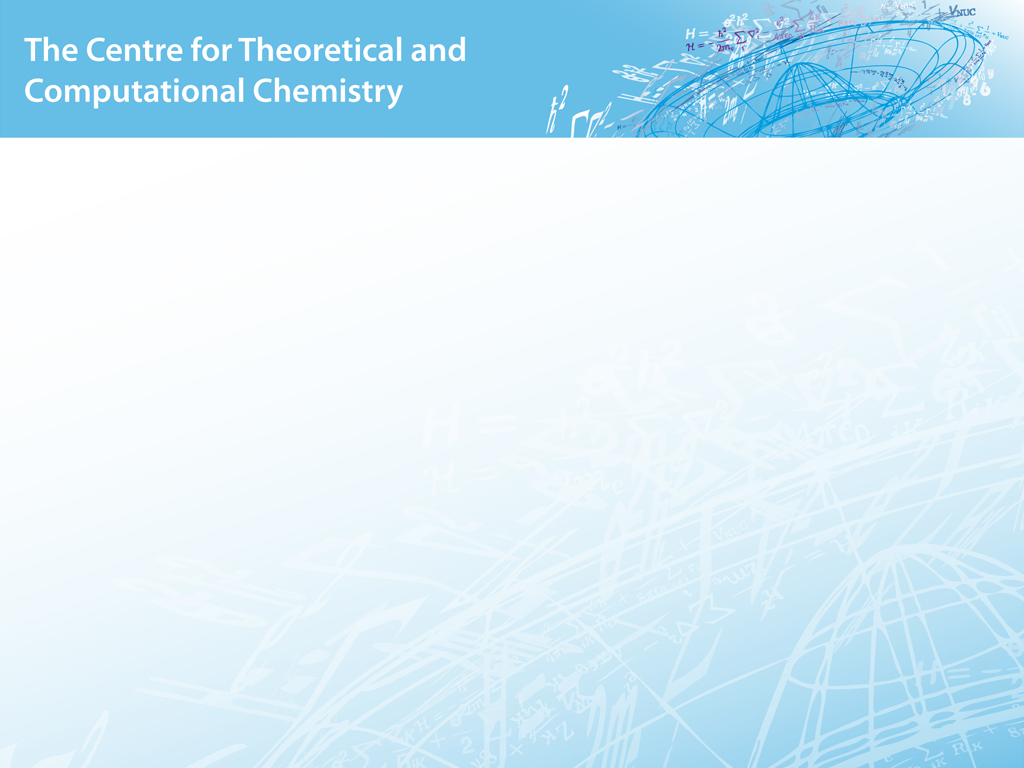
\includegraphics[width=1.02\paperwidth]{../templets/ctcc_forside.jpg}}
\maketitle
}

\begin{frame}
    \frametitle{Outlook}
    \begin{itemize}
	\item   Paper I
	\begin{itemize}
	    \item   Multiwavelets
	    \item   Function representations
	    \item   Decreasing order basis
	    \item   Results
	\end{itemize}
	\item   Paper II
	\begin{itemize}
	    \item   Parallel implementation
	    \item   Operator representation
	    \item   Coulomb interaction
	    \item   Results
	\end{itemize}
	\item   Paper III
	\begin{itemize}
	    \item   Density Functional Theory
	    \item   Integral formulation
	    \item   Iterative algorithm
	    \item   Results
	\end{itemize}
    \end{itemize}
\end{frame}

\begin{frame}
    \frametitle{Multiwavelets}
    Scaling/wavelet functions
\end{frame}

\begin{frame}
    \frametitle{Multiwavelets}
    Function representation\\
    Projection of orbital
\end{frame}

\begin{frame}
    \frametitle{Multiwavelets}
    Paper I
\end{frame}

\begin{frame}
    \frametitle{Parallel programming}
    Why parallel processing?
    \begin{itemize}
	\item	To get more processing power
	\item	To get more available memory
	\item	Future $\rightarrow$ \emph{more} processors rather than faster
    \end{itemize}
    \ \\
    \ \\
    \ \\
    Parallelization means
    \begin{itemize}
	\item	\textbf{distributing work} to processors
	\item	\textbf{syncronization} of distributed work
	\item	\textbf{distributing data} (if memory is distributed)
	\item	\textbf{communication} of distributed data
    \end{itemize}
\end{frame}

\begin{frame}
    \frametitle{Shared memory (OpenMP)}
    \begin{minipage}[b]{0.45\linewidth}
	Pros
	\begin{itemize}
	    \item Relatively simple implementation
	    \item Quick way to good performance
	    \item No communication
	    \item Simple load balance
	\end{itemize}
	Cons
        \begin{itemize}
	    \item Small to medium scale parallelization
	    \item Limited memory
	    \item Race conditions
	    \item Tedious debugging (Heisenbugs)
	\end{itemize}
    \end{minipage}
    \hfill
    \begin{minipage}[b]{0.4\linewidth}
	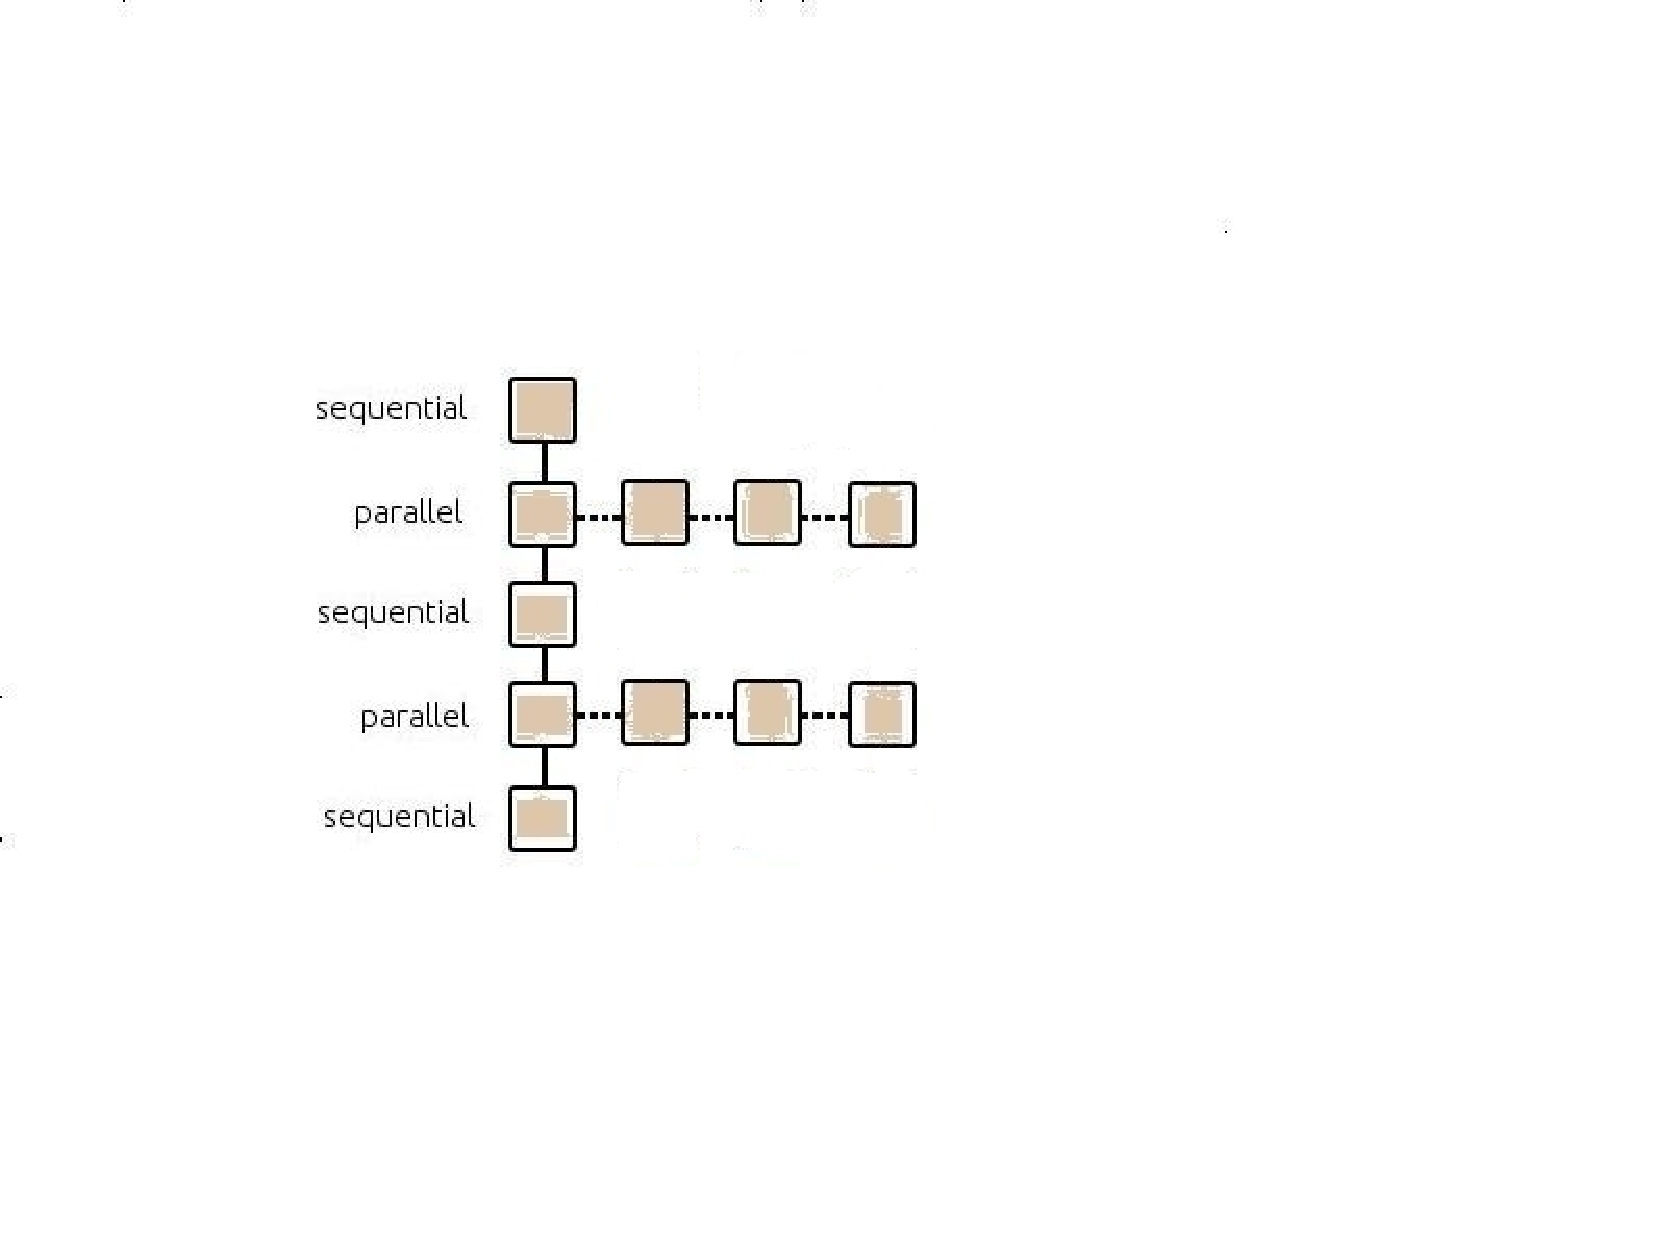
\includegraphics[viewport = 120 160 460 450, clip, scale=0.4]{figures/parallel_OMP.pdf}
	\ \\
	\ \\
	\ \\
	\ \\
    \end{minipage}
\end{frame}

\begin{frame}
    \frametitle{Distributed memory (MPI)}
    \begin{minipage}[b]{0.45\linewidth}
	pros
	\begin{itemize}
	    \item large scale parallelization
	    \item extensive memory
	\end{itemize}
	cons
	\begin{itemize}
	    \item complicated implementation
	    \item user specified work/data decomposition 
	    \item user specified communication
	    \item difficult to load balance
	    \item communication overhead
	\end{itemize}
    \end{minipage}
    \hfill
    \begin{minipage}[b]{0.4\linewidth}
	\only<1>{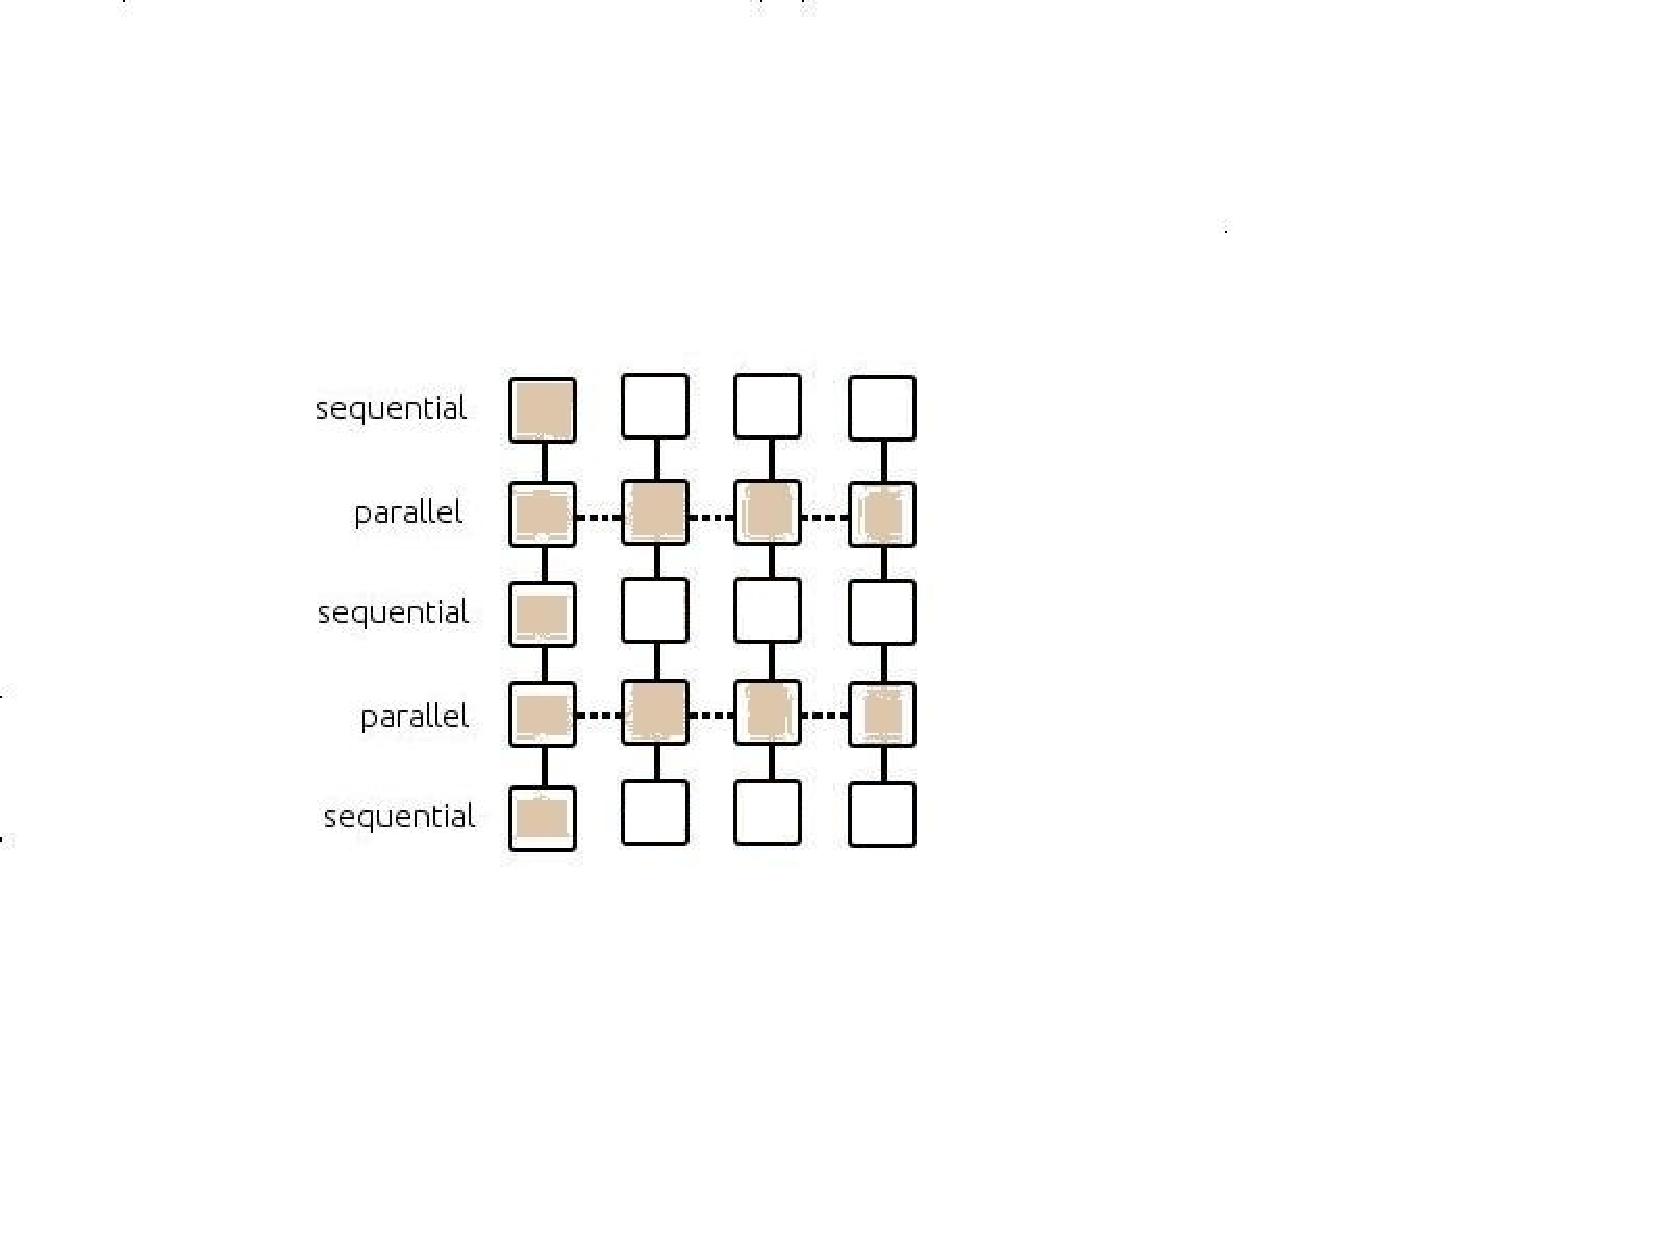
\includegraphics[viewport = 120 160 460 450, clip, scale=0.4]{figures/parallel_mpi_1.pdf}
	\ \\
	}
	\only<2>{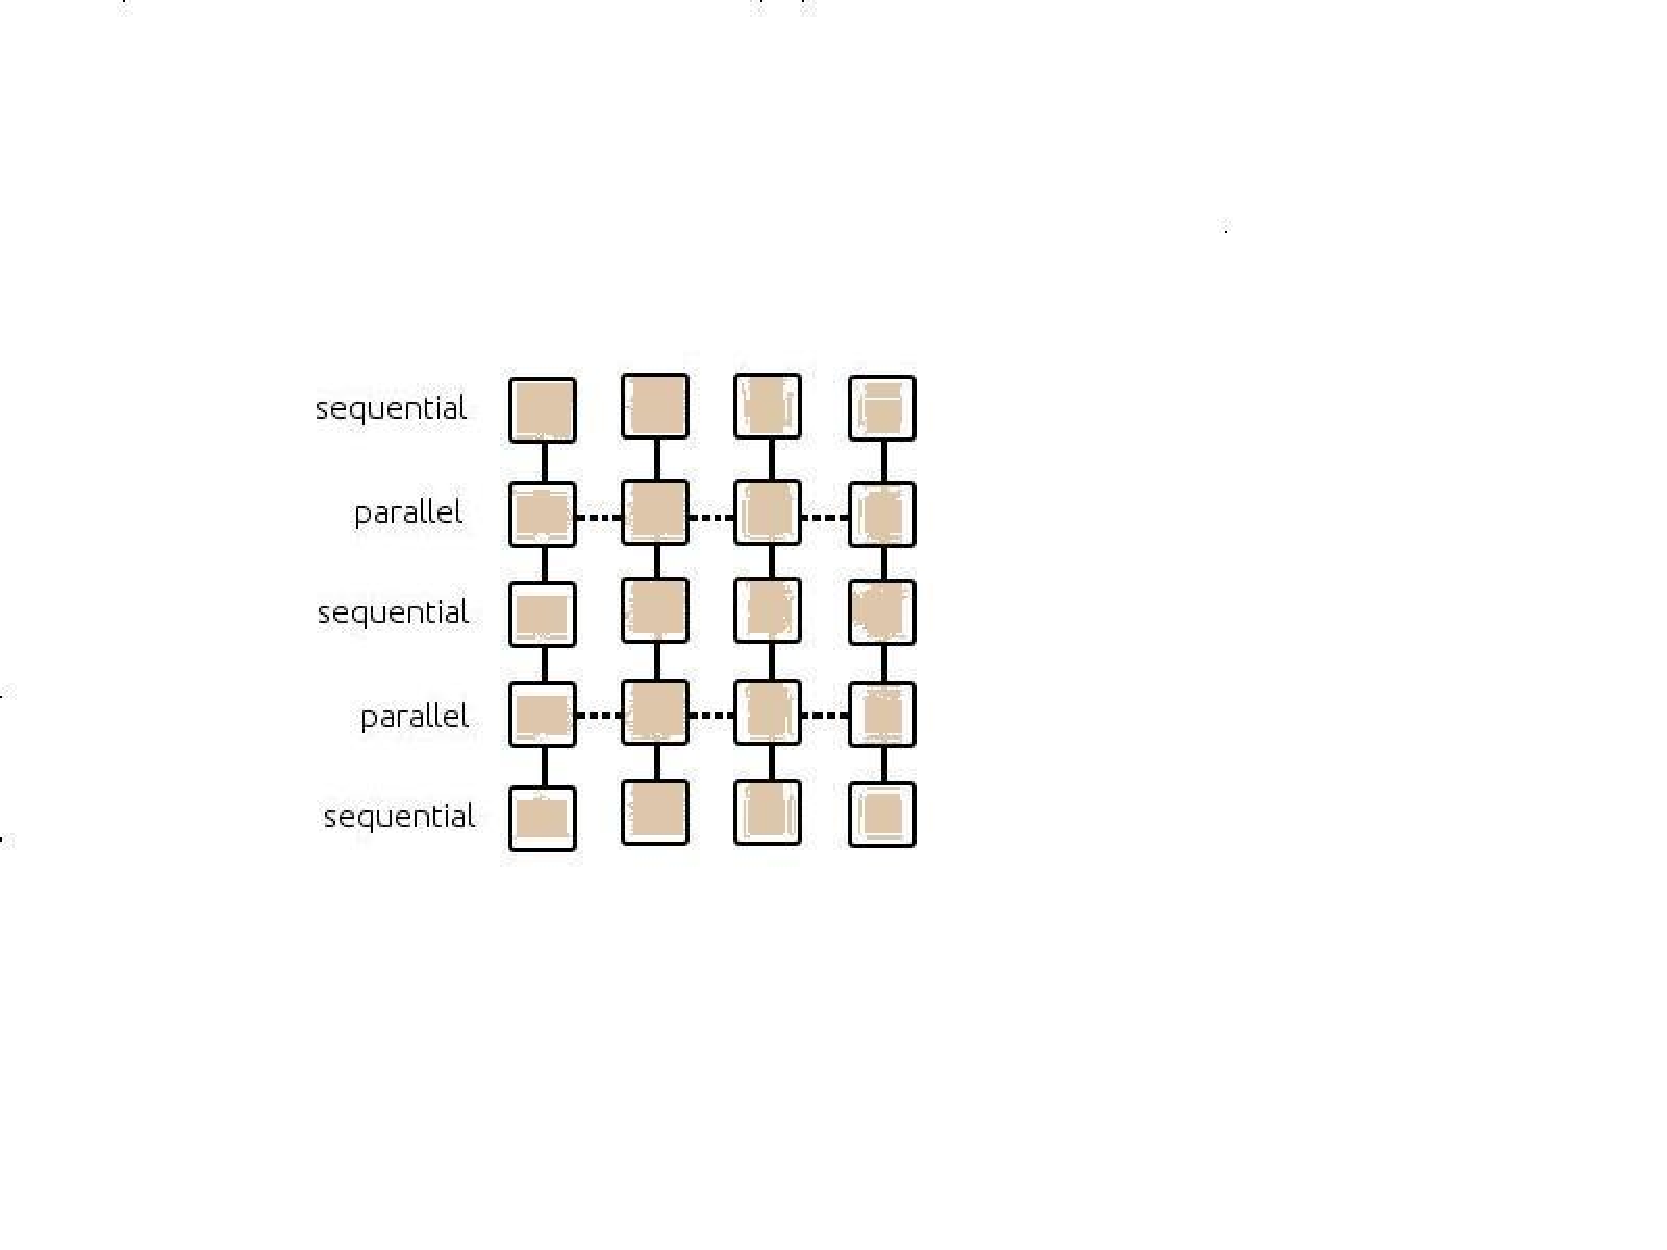
\includegraphics[viewport = 120 160 460 450, clip, scale=0.4]{figures/parallel_mpi_2.pdf}
	\ \\
	}
    \end{minipage}
\end{frame}

\begin{frame}
    \frametitle{Parallel efficiency}
    \begin{center}
    \only<1>{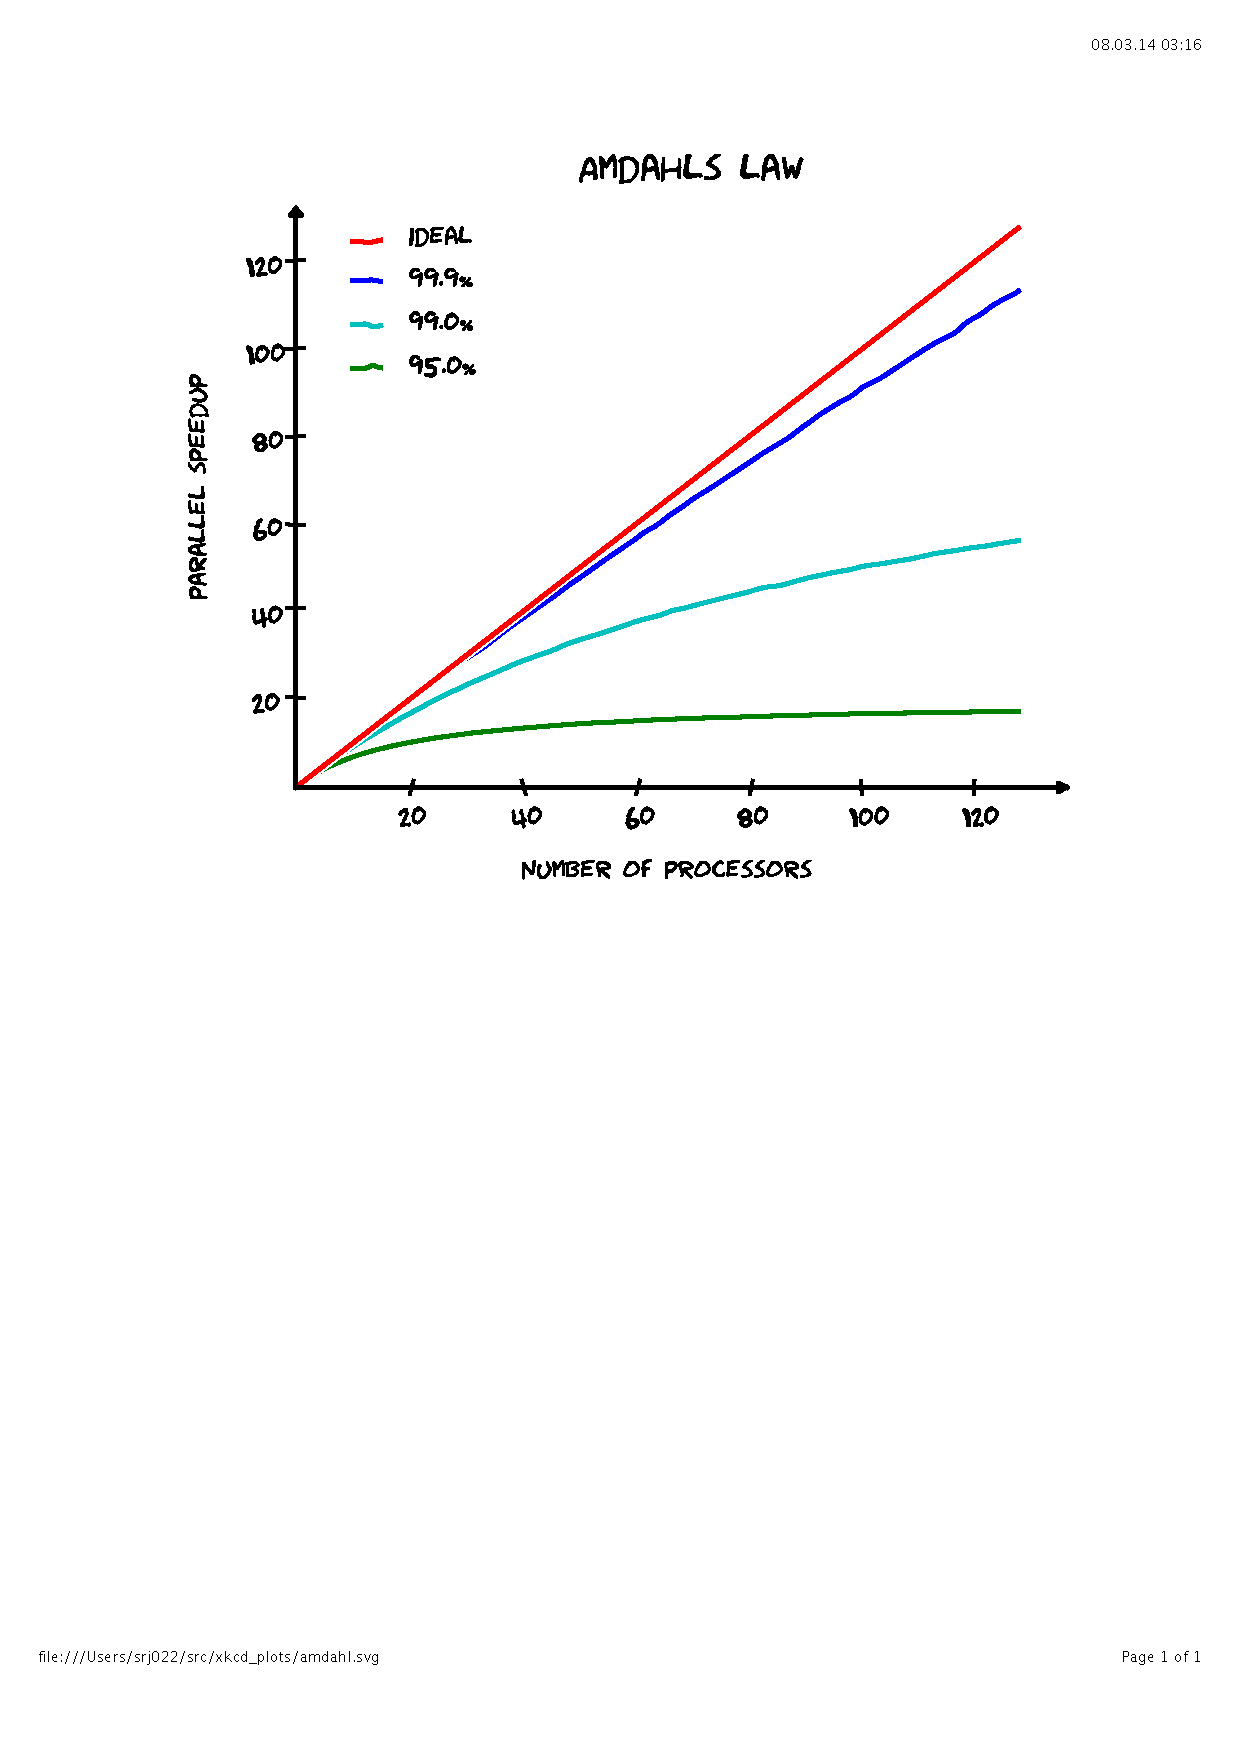
\includegraphics[clip, viewport = 50 250 550 800, scale=0.5]{figures/amdahl.pdf}}
    \only<2>{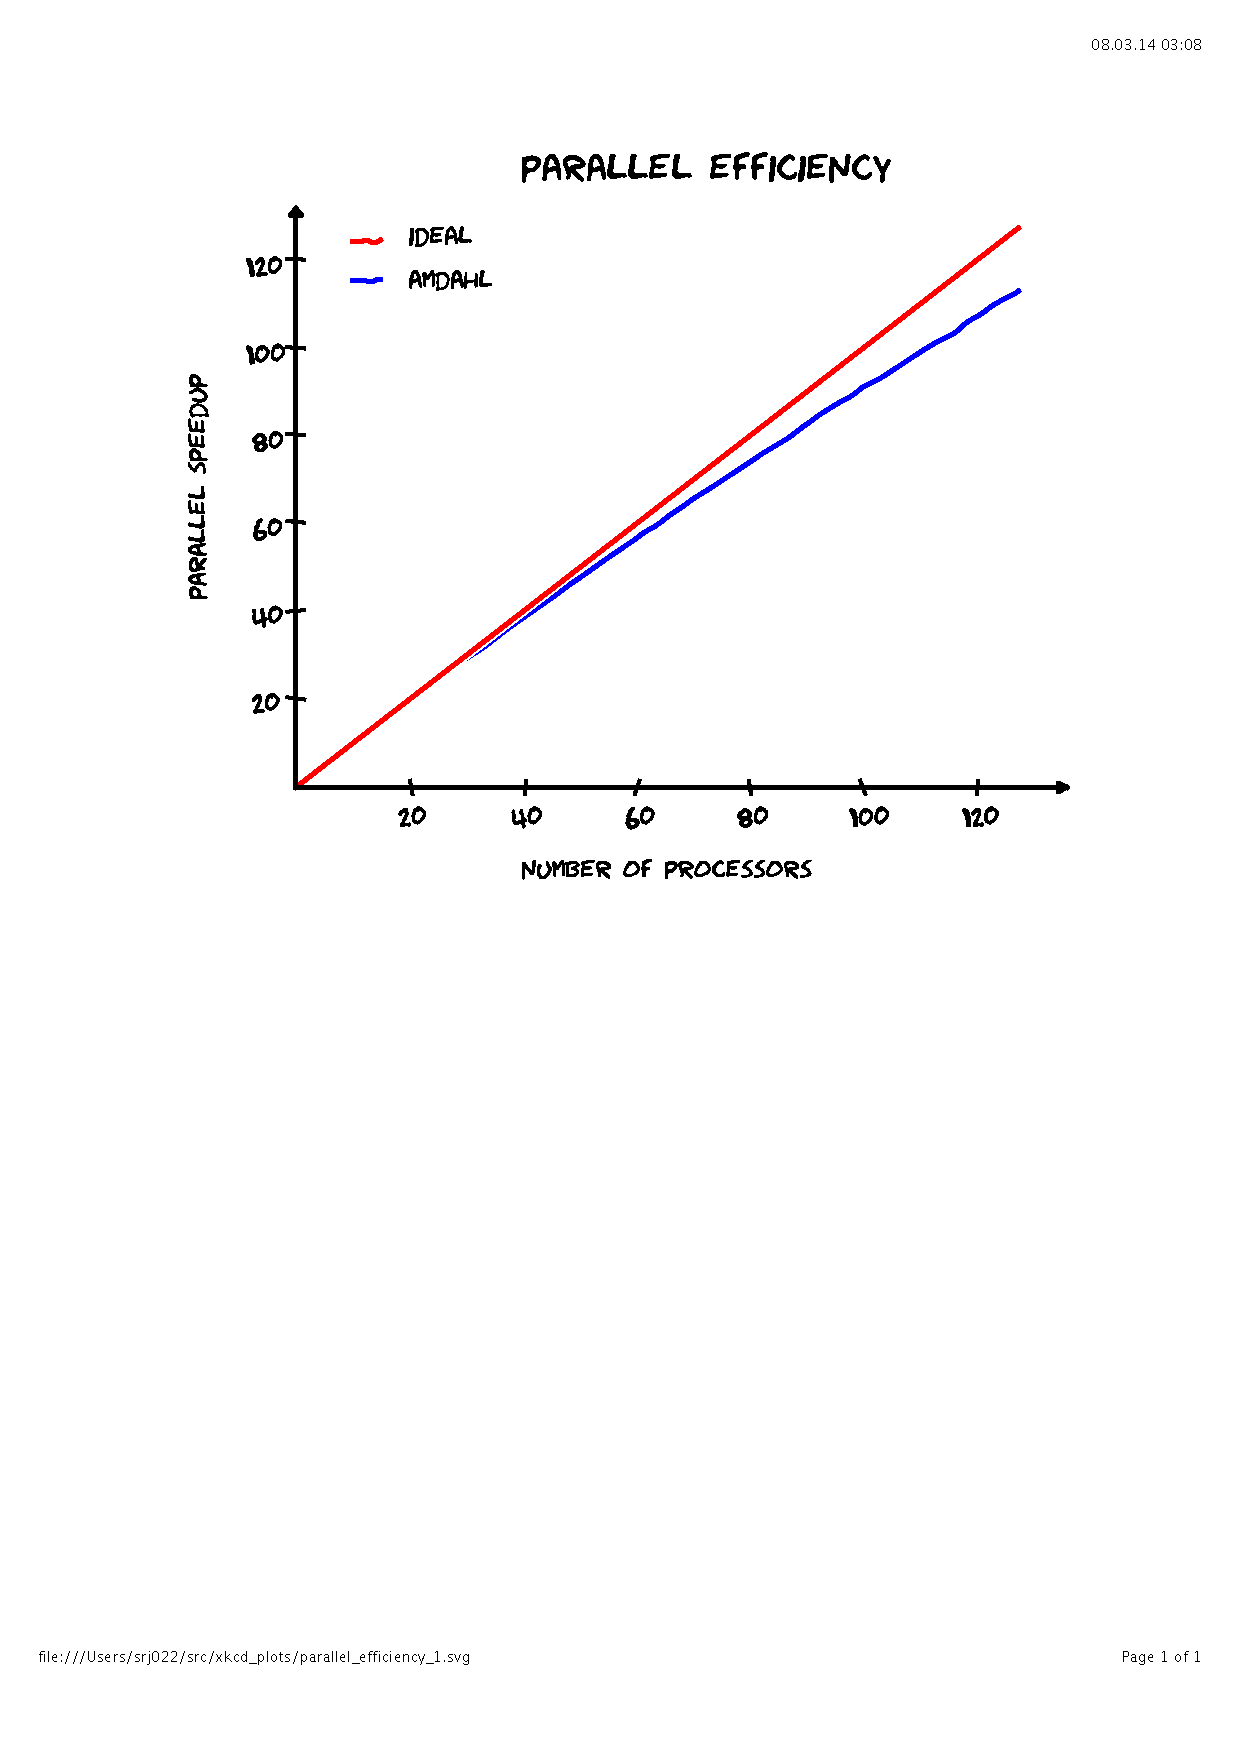
\includegraphics[clip, viewport = 50 250 550 800, scale=0.5]{figures/parallel_efficiency_1.pdf}}
    \only<3>{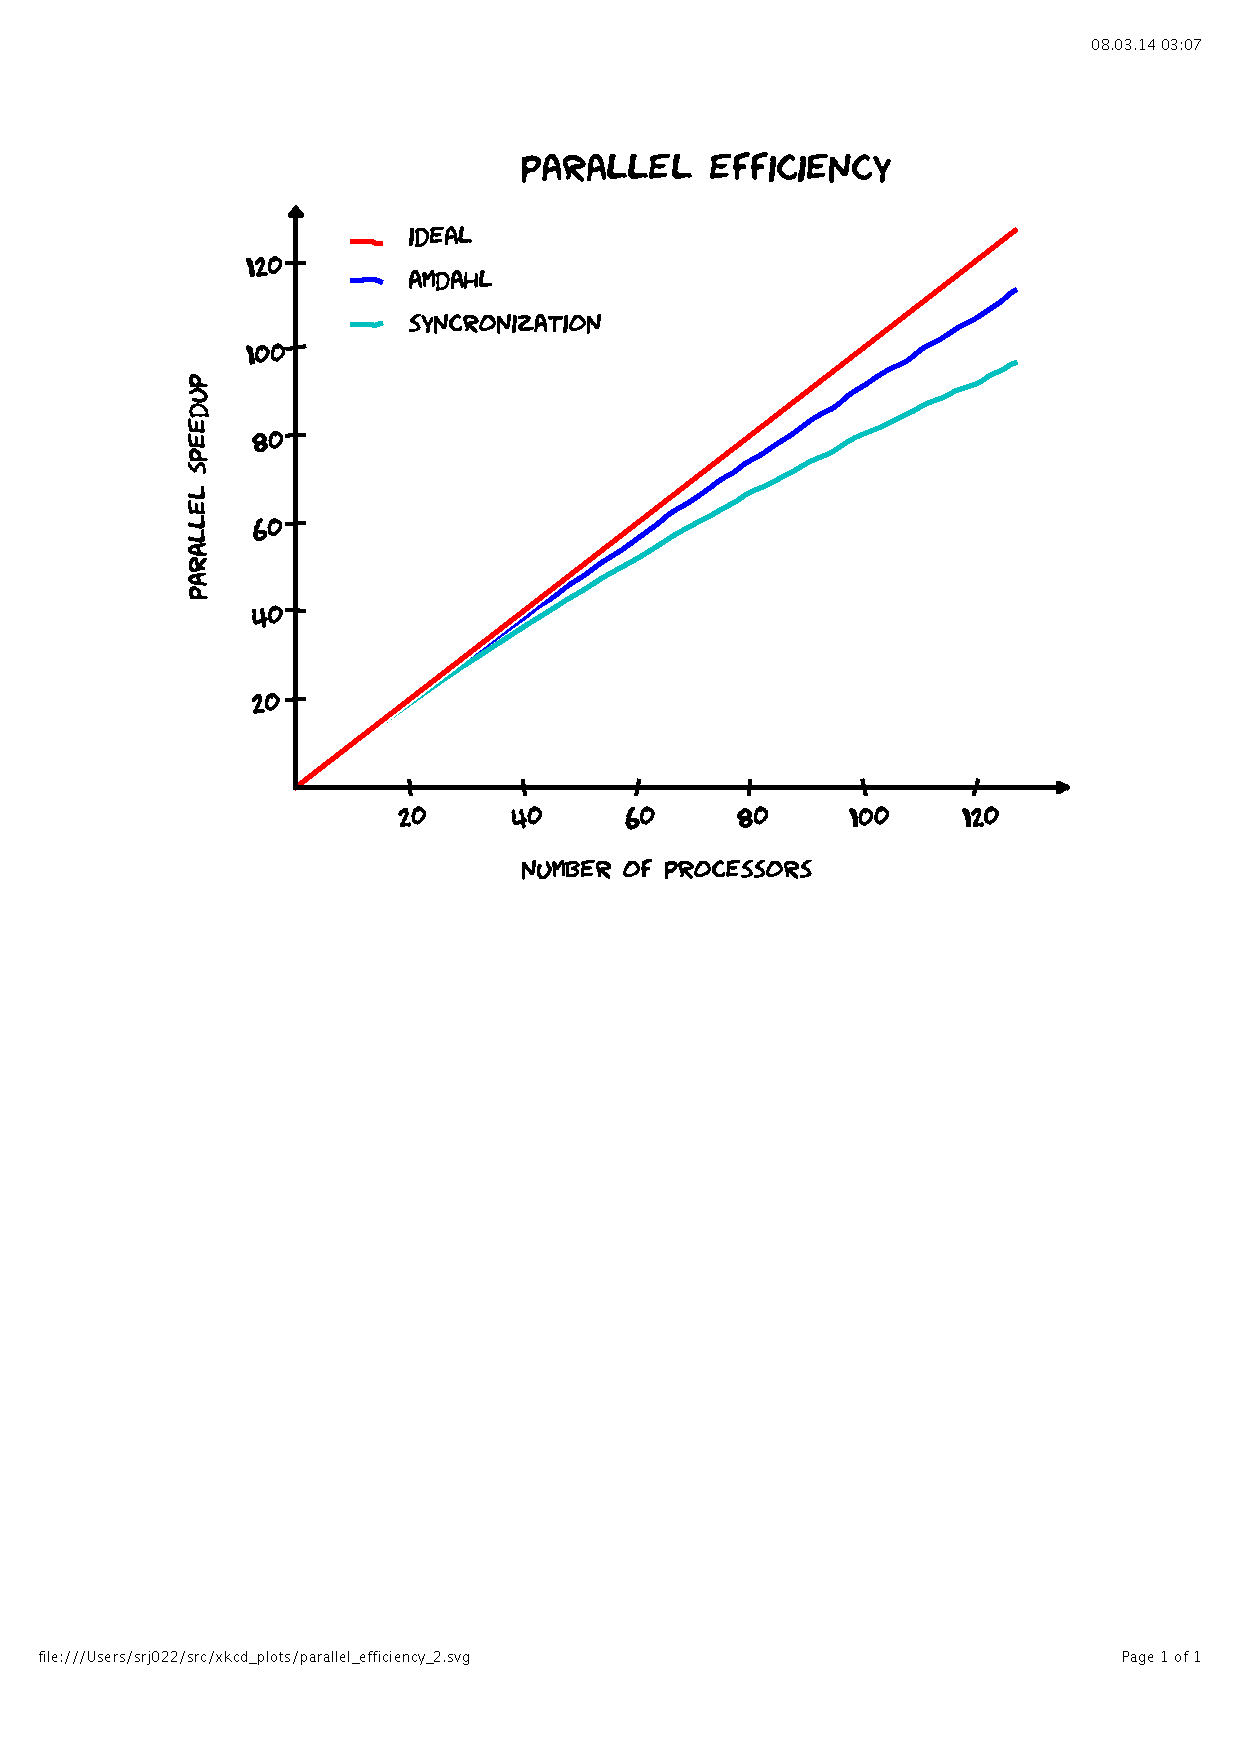
\includegraphics[clip, viewport = 50 250 550 800, scale=0.5]{figures/parallel_efficiency_2.pdf}}
    \only<4>{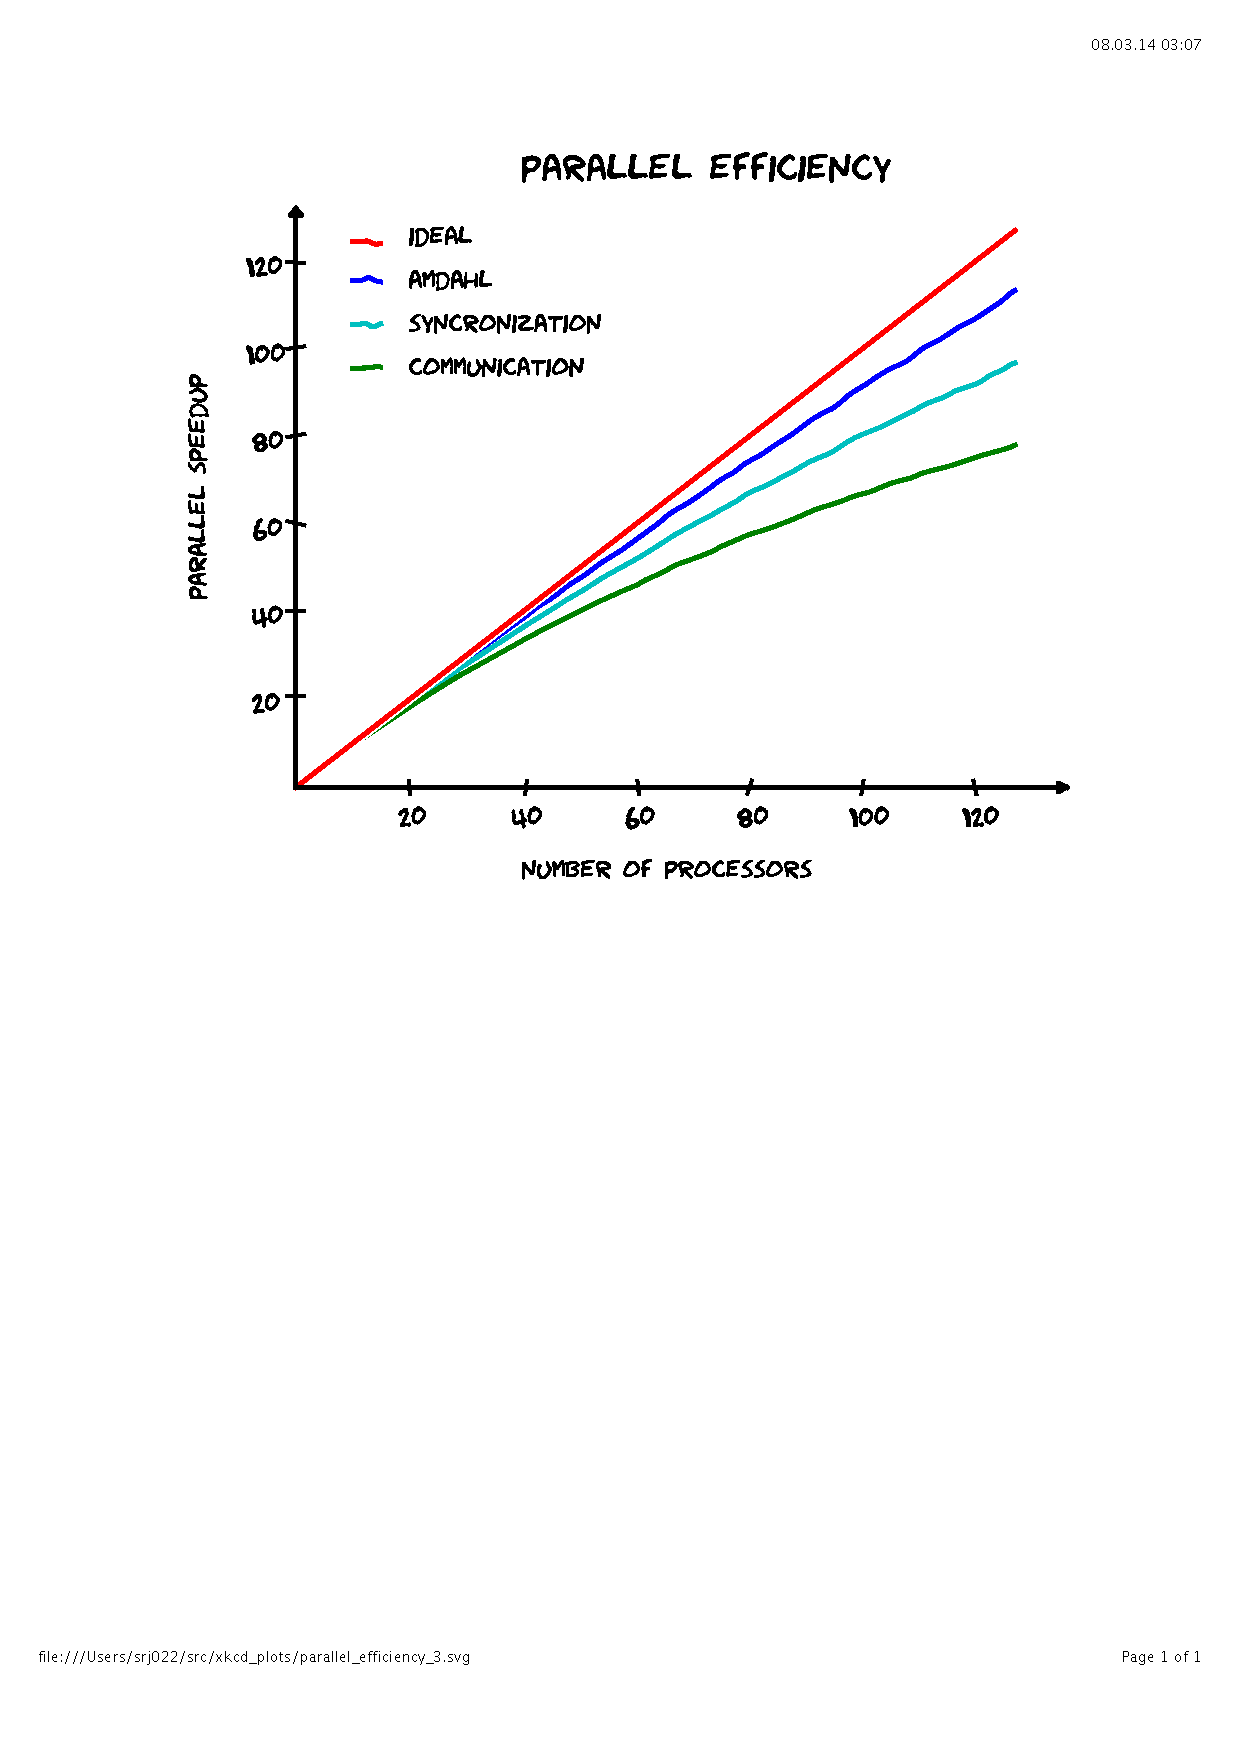
\includegraphics[clip, viewport = 50 250 550 800, scale=0.5]{figures/parallel_efficiency_3.pdf}}
    \end{center}
\end{frame}

\begin{frame}
    \frametitle{Data distribution}
    \begin{minipage}[b]{0.40\linewidth}
	Lebesgue
	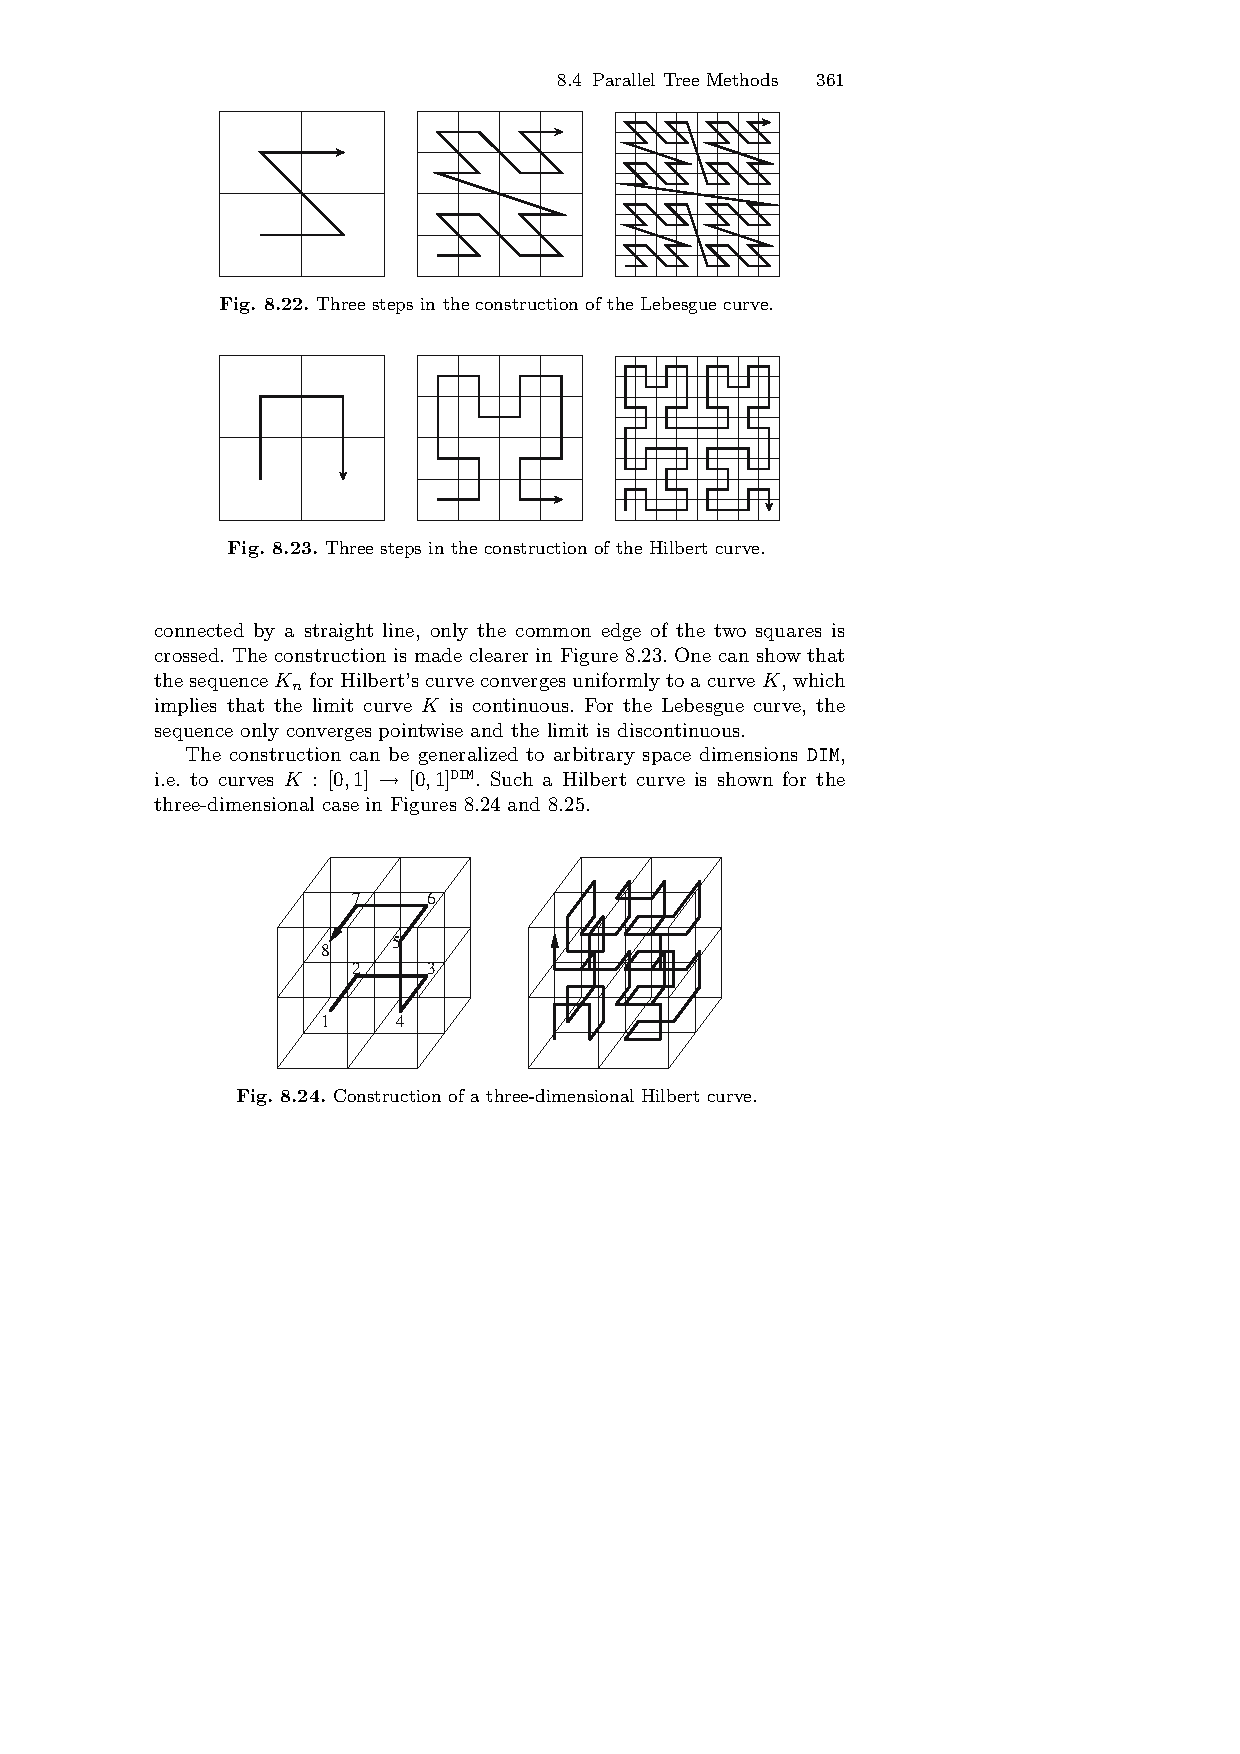
\includegraphics[viewport = 105 705 375 795, scale=0.6, clip]{figures/hilbertCurve.pdf}
	\ \\
	Hilbert
	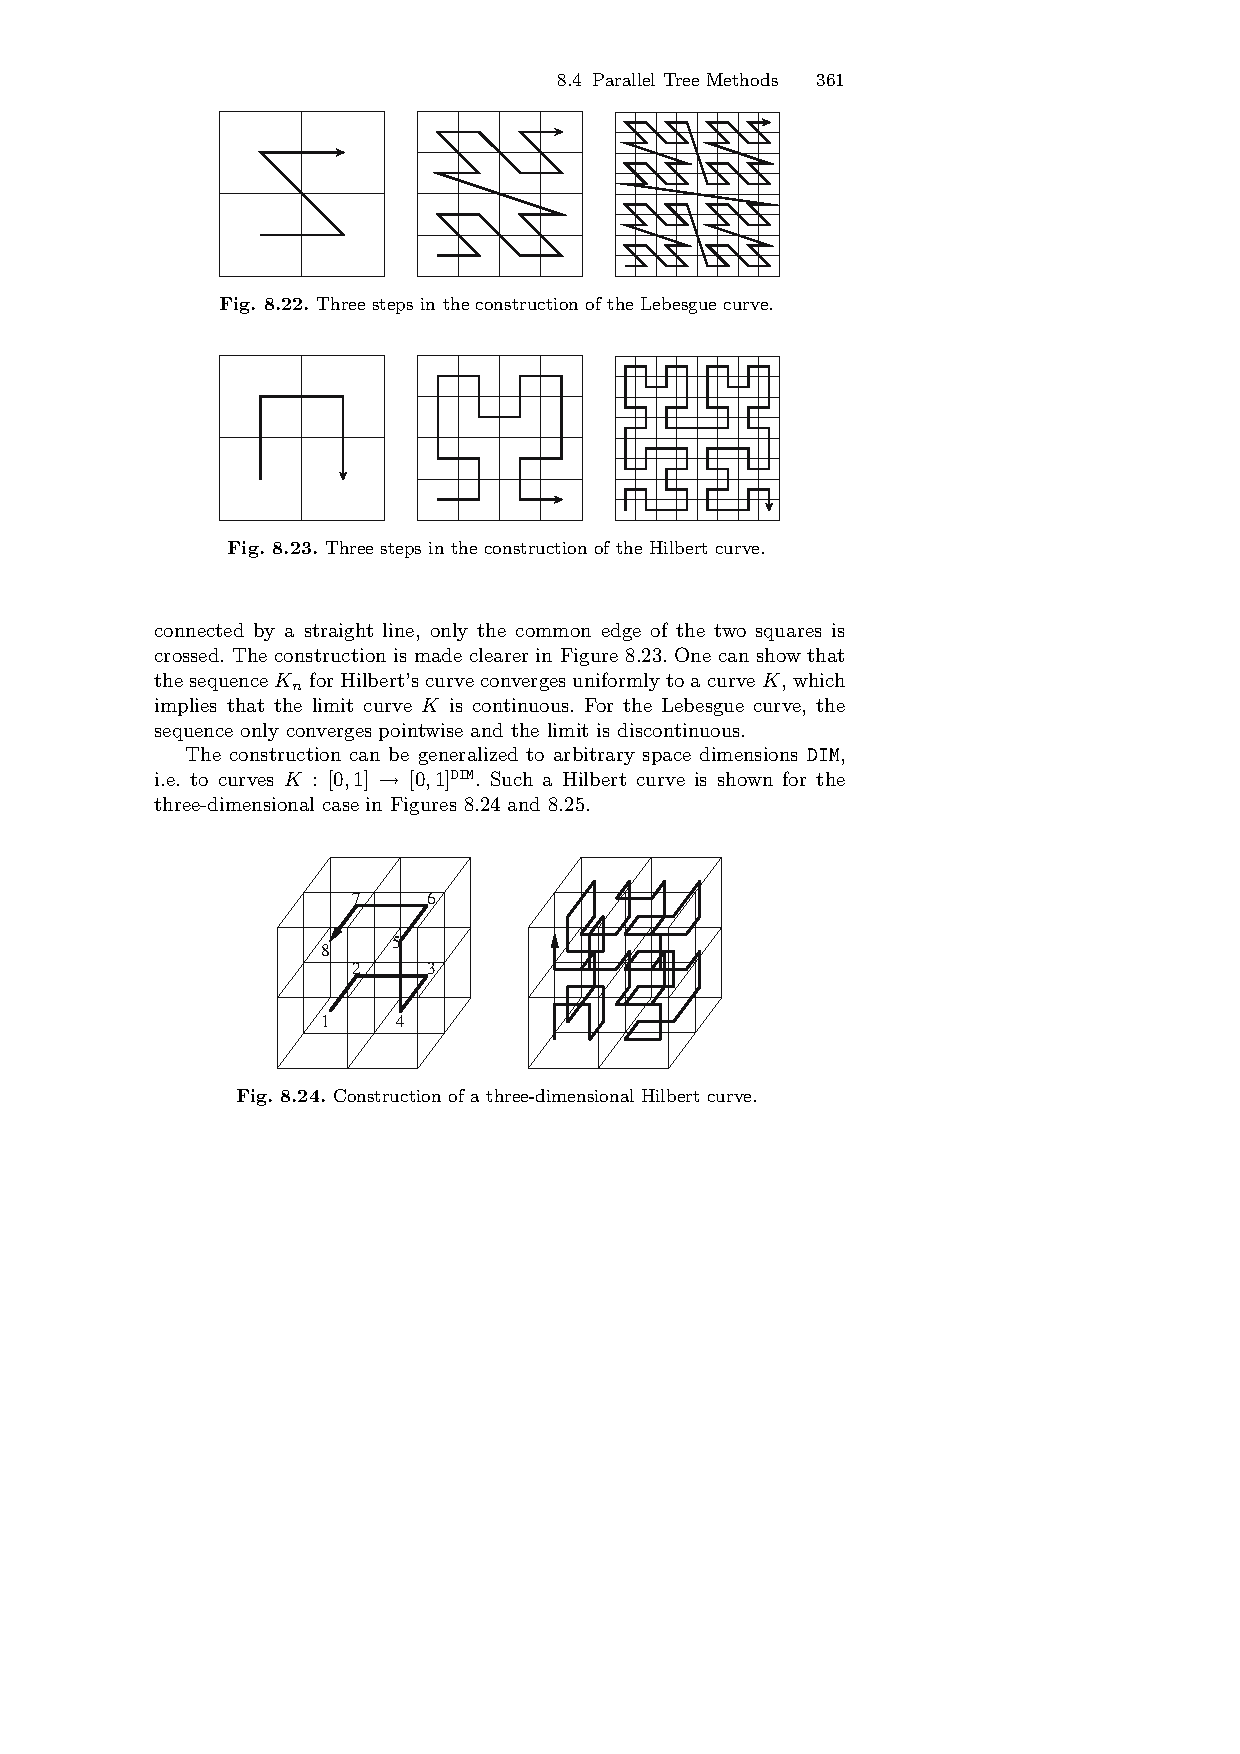
\includegraphics[viewport = 105 590 375 680, scale=0.6, clip]{figures/hilbertCurve.pdf}
	\ \\
	3D
	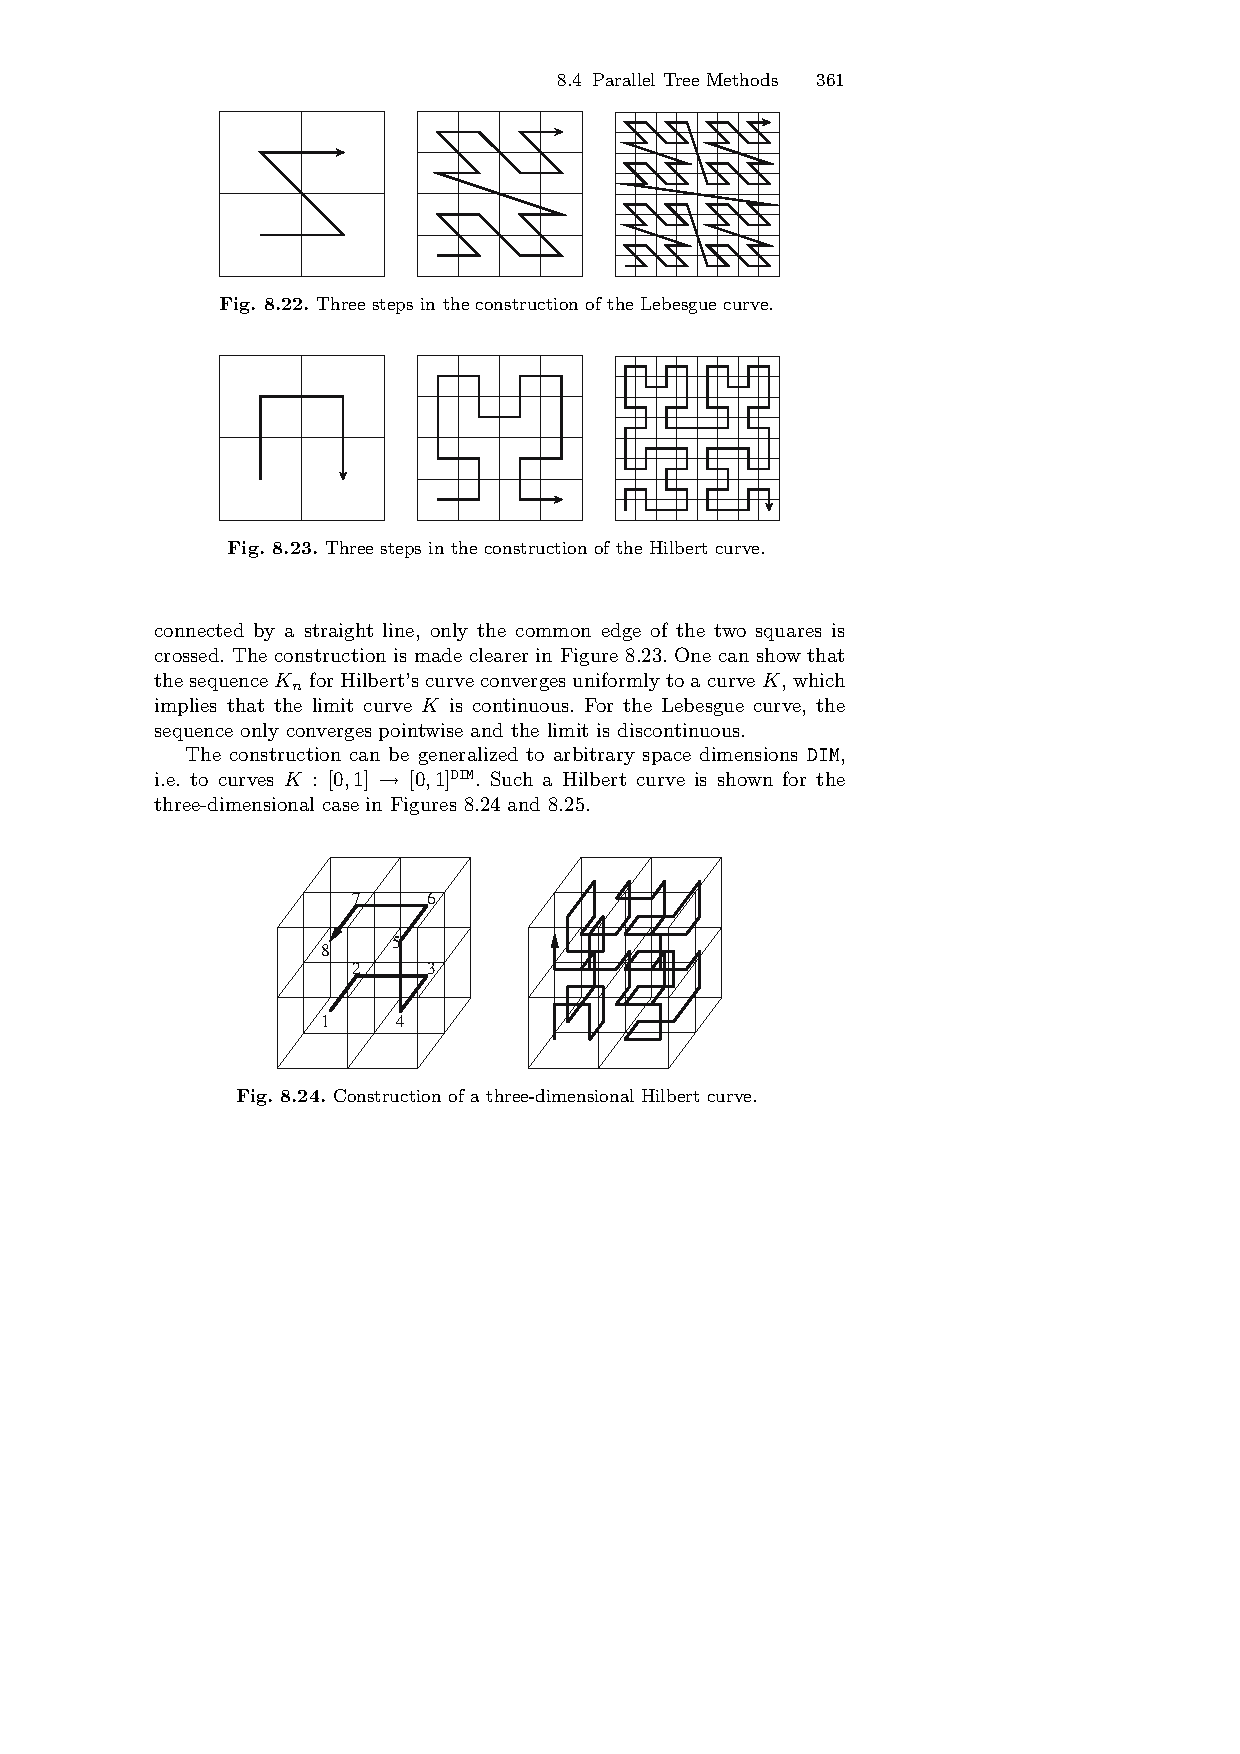
\includegraphics[viewport = 105 325 375 435, scale=0.6, clip]{figures/hilbertCurve.pdf}
    \end{minipage}
    \hfill
    \begin{minipage}[b]{0.4\linewidth}
	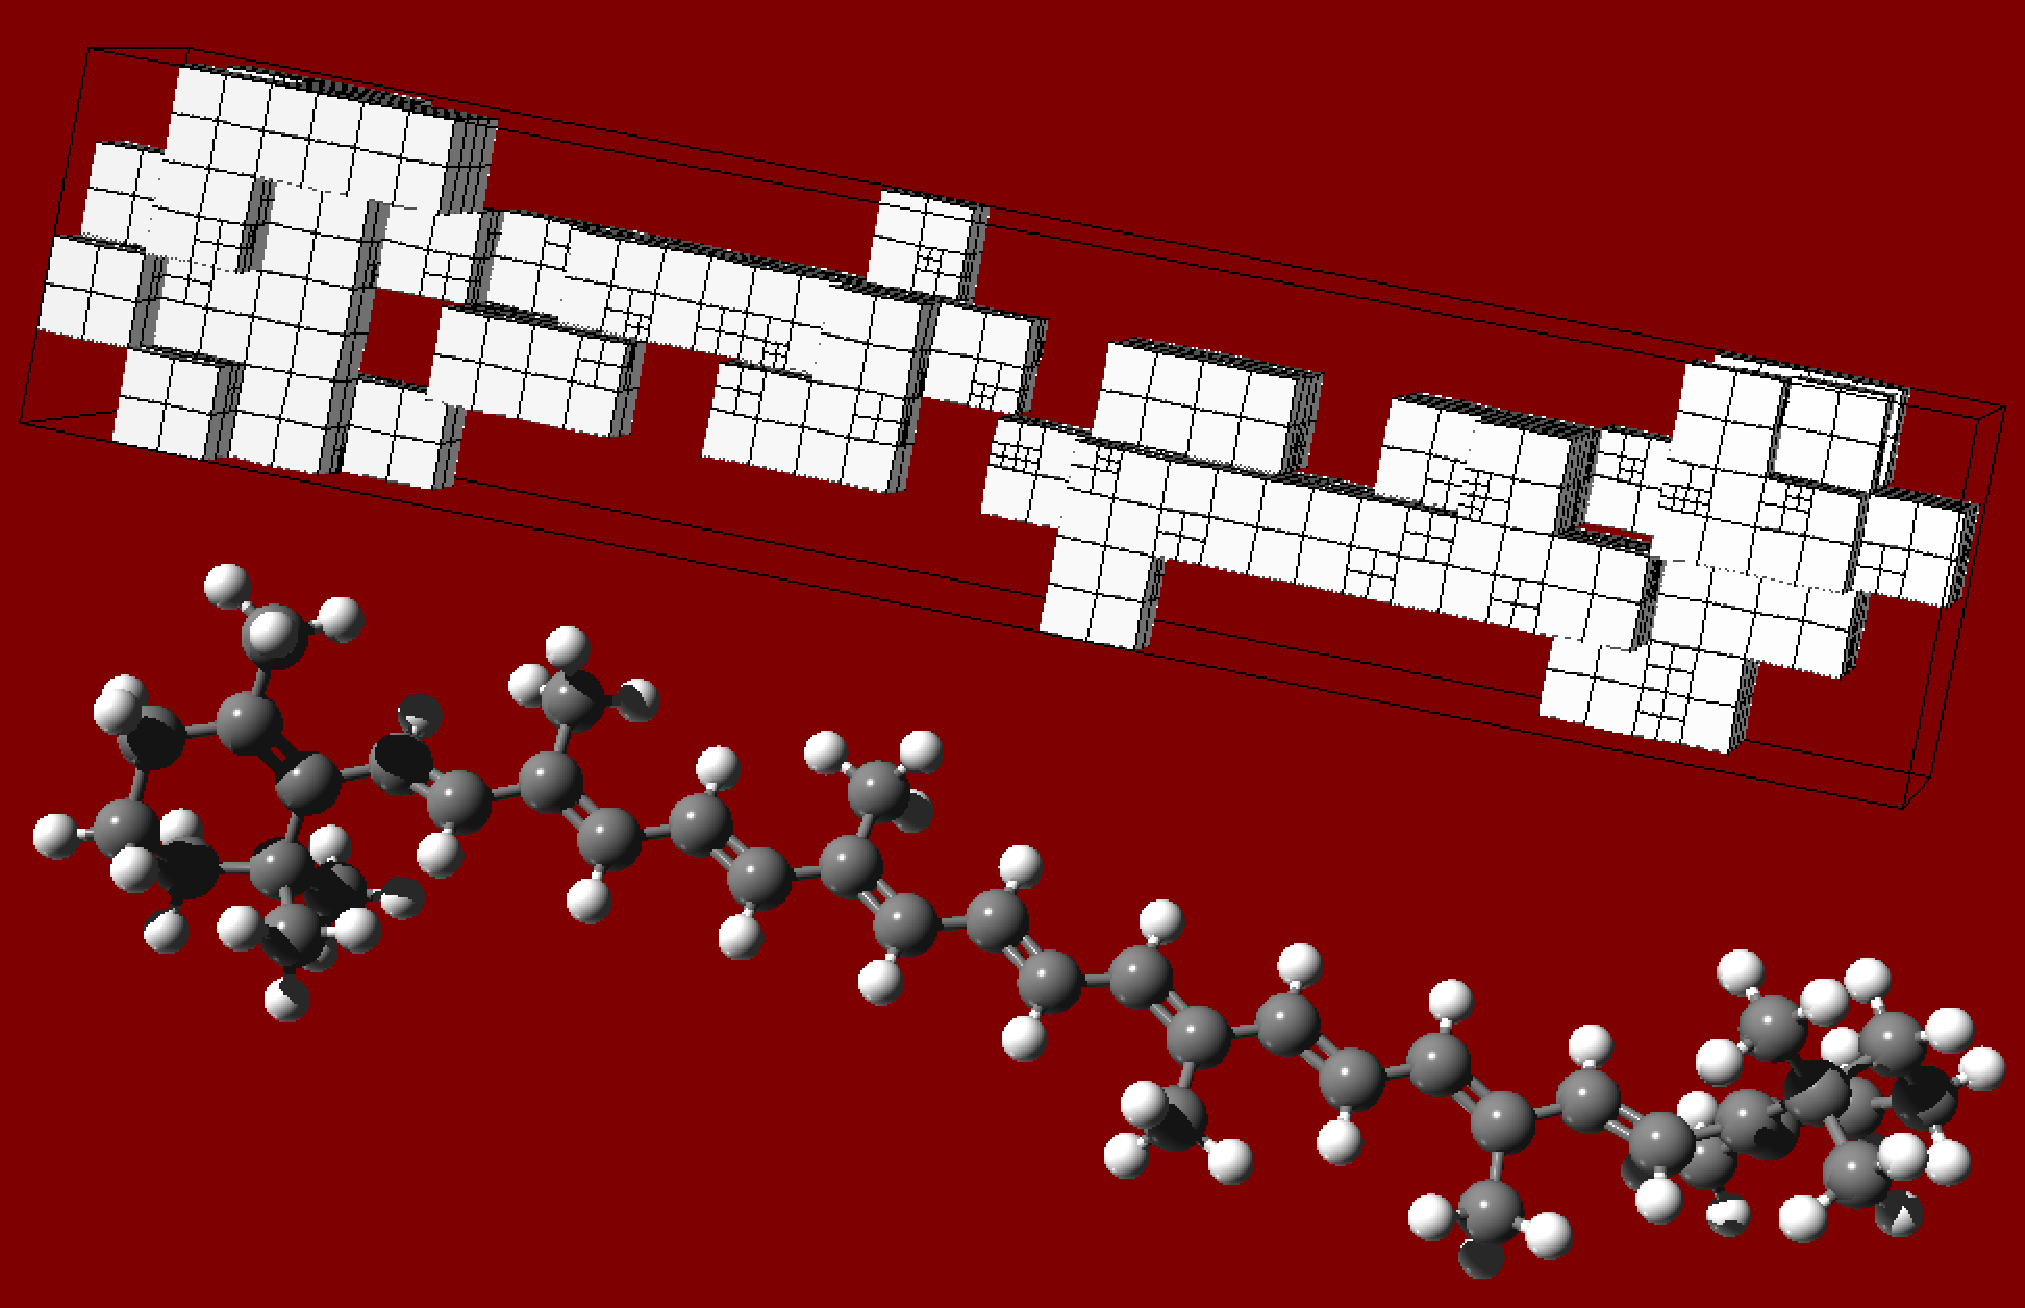
\includegraphics[angle=90, scale=0.2]{figures/caroteneGrid.pdf}
    \end{minipage}
\end{frame}

\begin{frame}
    \frametitle{Operator representation}
    The multiwavelet basis is well suited for integral operators
    \begin{equation}
	\nonumber
	g(\boldsymbol{r}) = \int K(\boldsymbol{r} - \boldsymbol{r'}) 
	    f(\boldsymbol{r'}) d\boldsymbol{r'}
    \end{equation}
    \ \\
    We have specifically implemented three such operators
    \ \\
    \begin{columns}
    \begin{column}{.48\textwidth}
    \begin{itemize}
	\item Poisson kernel (electrostatics)
	    \ \\
	    \ \\
	    \ \\
	\item Bound-State Helmholtz (BSH) kernel (DFT equations)
	    \ \\
	    \ \\
	    \ \\
	\item Derivative kernel
    \end{itemize}
    \end{column}
    \begin{column}{.48\textwidth}
    \ \\
    \begin{equation}
	\nonumber
	\scriptsize
	P(\boldsymbol{r}-\boldsymbol{r}') = 
	    \frac{1}{4\pi}\ \frac{1}{|\boldsymbol{r}-\boldsymbol{r}'|}
    \end{equation}
    \ \\
    \ \\
    \begin{equation}
	\nonumber
	\scriptsize
	H^{\mu}(\boldsymbol{r}-\boldsymbol{r}') = \frac{1}{4\pi}\ 
	    \frac{e^{-\mu |\boldsymbol{r}-\boldsymbol{r}'|}}{|\boldsymbol{r}-\boldsymbol{r}'|}
    \end{equation}
    \ \\
    \ \\
    \begin{equation}
	\nonumber
	\scriptsize
	D^x(x-x') = \frac{d}{dx} \delta(x - x')
    \end{equation}
    \end{column}
    \end{columns}    
\end{frame}

\begin{frame}
    \frametitle{Coulomb interaction}
    Coulomb potential for point charge in position $\boldsymbol{r}'$
    \begin{equation}
    	\nonumber
    	V(\boldsymbol{r}) = \frac{q}{4\pi\epsilon_0}
    	\frac{1}{|\boldsymbol{r}-\boldsymbol{r'}|}
    \end{equation}
    \ \\
    Poisson's equation for arbitrary charge densities (in atomic units)
    \begin{equation}
	\nonumber
    	\nabla^2 V(\boldsymbol{r}) = -\rho(\boldsymbol{r})
    \end{equation}
    \ \\
    can be solved directly through the integral formulation using the Poisson kernel
    \begin{equation}
	\nonumber
	V(\boldsymbol{r}) = 
	\int P(\boldsymbol{r}-\boldsymbol{r'})\rho(\boldsymbol{r'}) d\boldsymbol{r'} =
	\int\frac{\rho(\boldsymbol{r'})}{4\pi|\boldsymbol{r} - \boldsymbol{r'}|} d\boldsymbol{r'} 
    \end{equation}
    \ \\
    \pause
    Numerical problems
    \begin{itemize}
	\item Not separable in Cartesian coordinates
	\item Singularity at short-range
	\item Slow decay at long-range
    \end{itemize}
\end{frame}

\begin{frame}
    \frametitle{Separation of variables using Gaussians}
    \begin{columns}
    \begin{column}{.40\textwidth}
    \ \\
    \begin{equation}
	\nonumber
	\frac{1}{\boldsymbol{r}} \approx \sum_{i=1}^M a_i e^{-\alpha_i \boldsymbol{r}^2} 
    \end{equation}
    \ \\
    \ \\
    \ \\
    \ \\
    \ \\
    \begin{itemize}
	\item	Separates coordinates
	\item	Removes singularity
	\item	Separates length scales
    \end{itemize}
    \end{column}
    \begin{column}{.60\textwidth}
	\only<1>{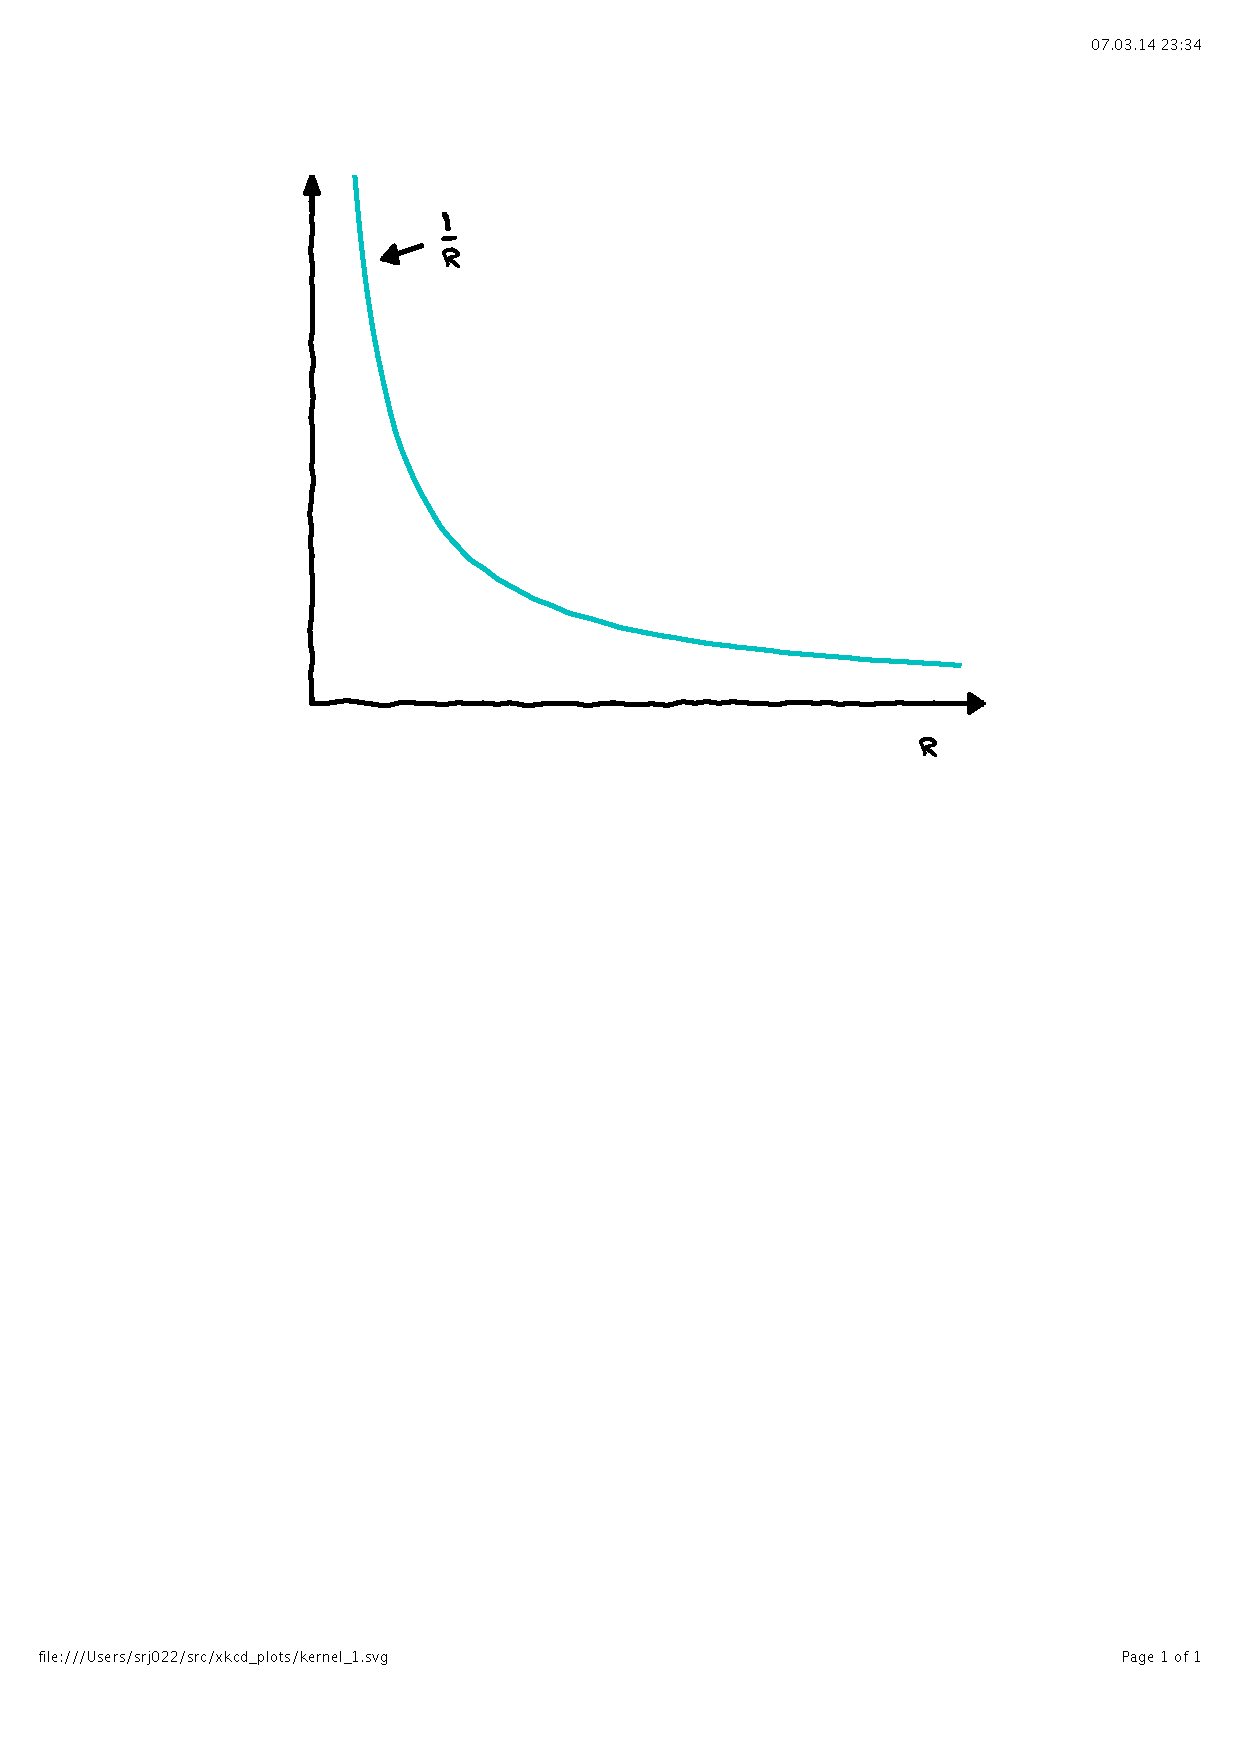
\includegraphics[scale=0.5, clip, viewport = 110 450 490 800]{figures/kernel_1.pdf}}
	\only<2>{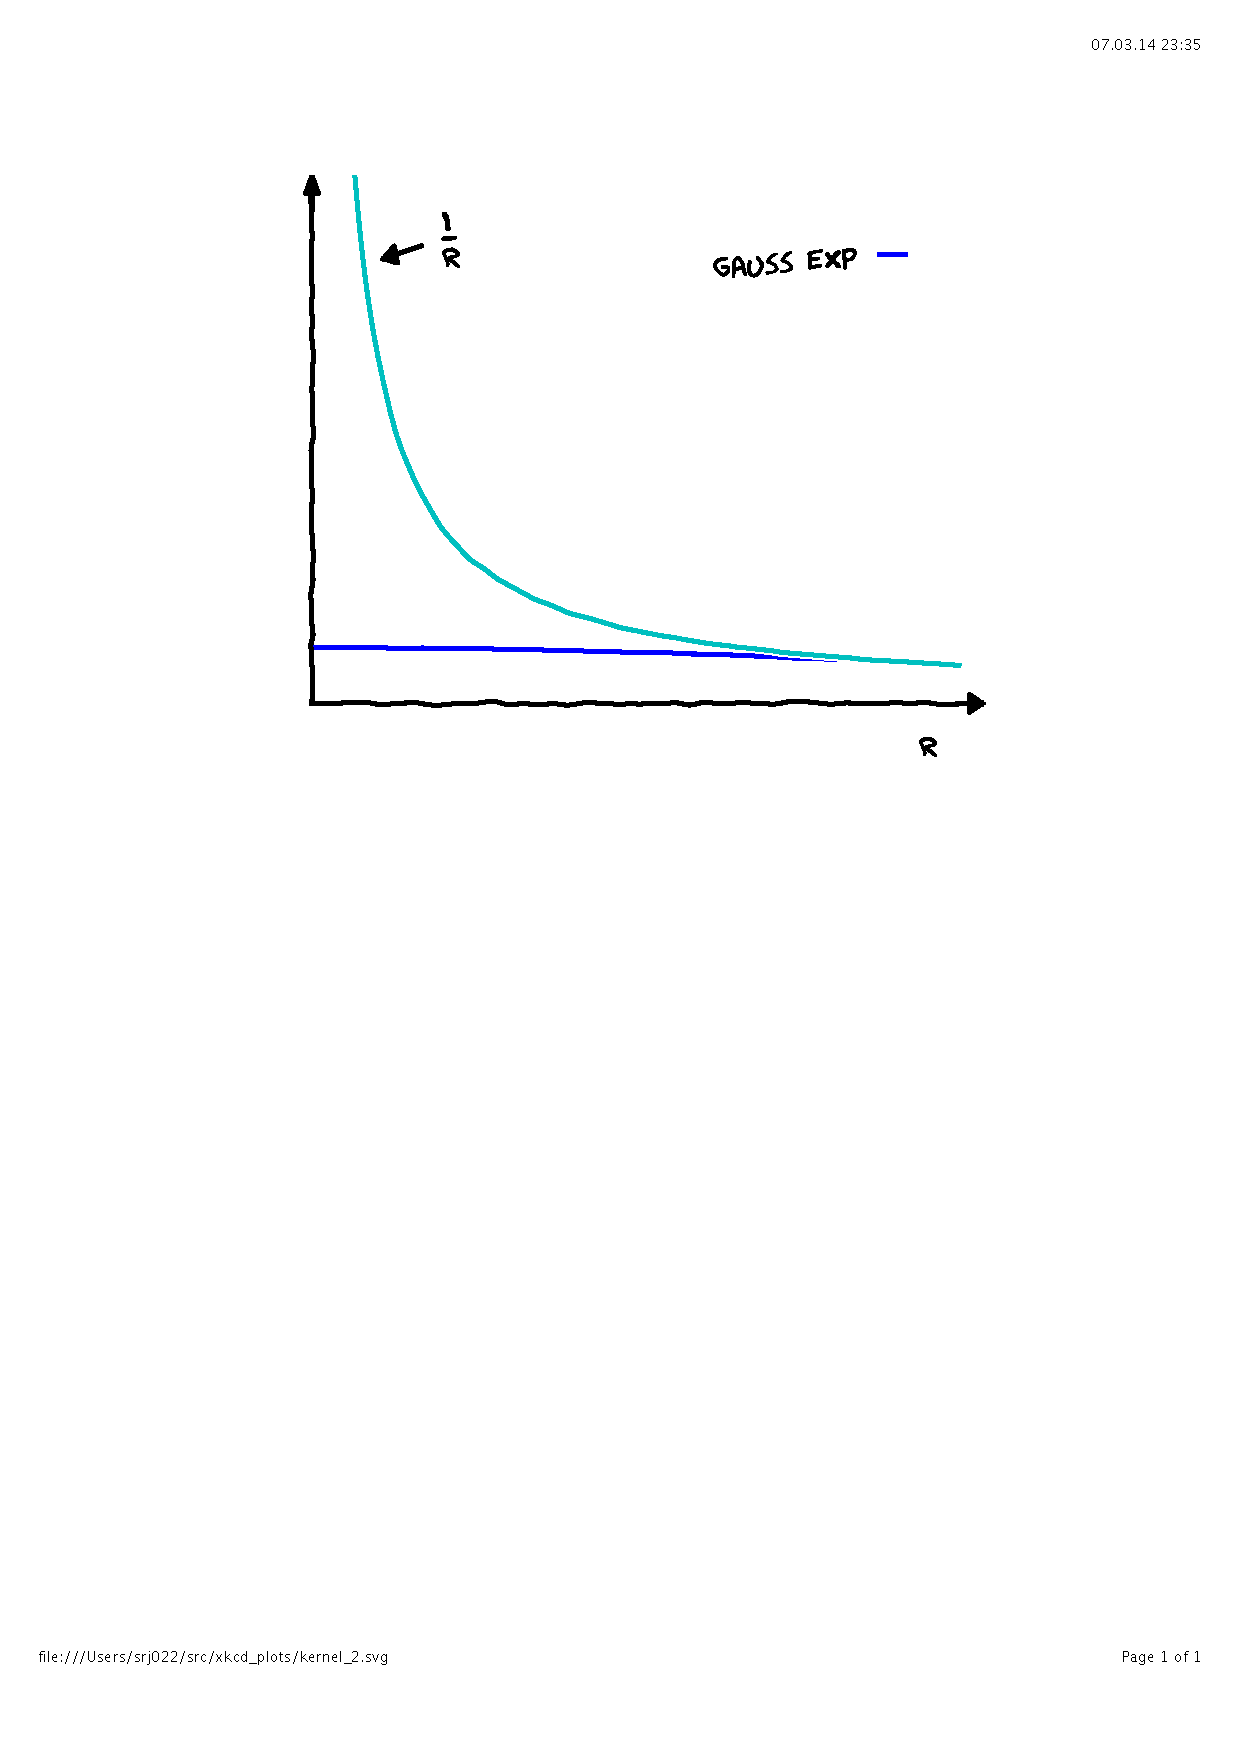
\includegraphics[scale=0.5, clip, viewport = 110 450 490 800]{figures/kernel_2.pdf}}
	\only<3>{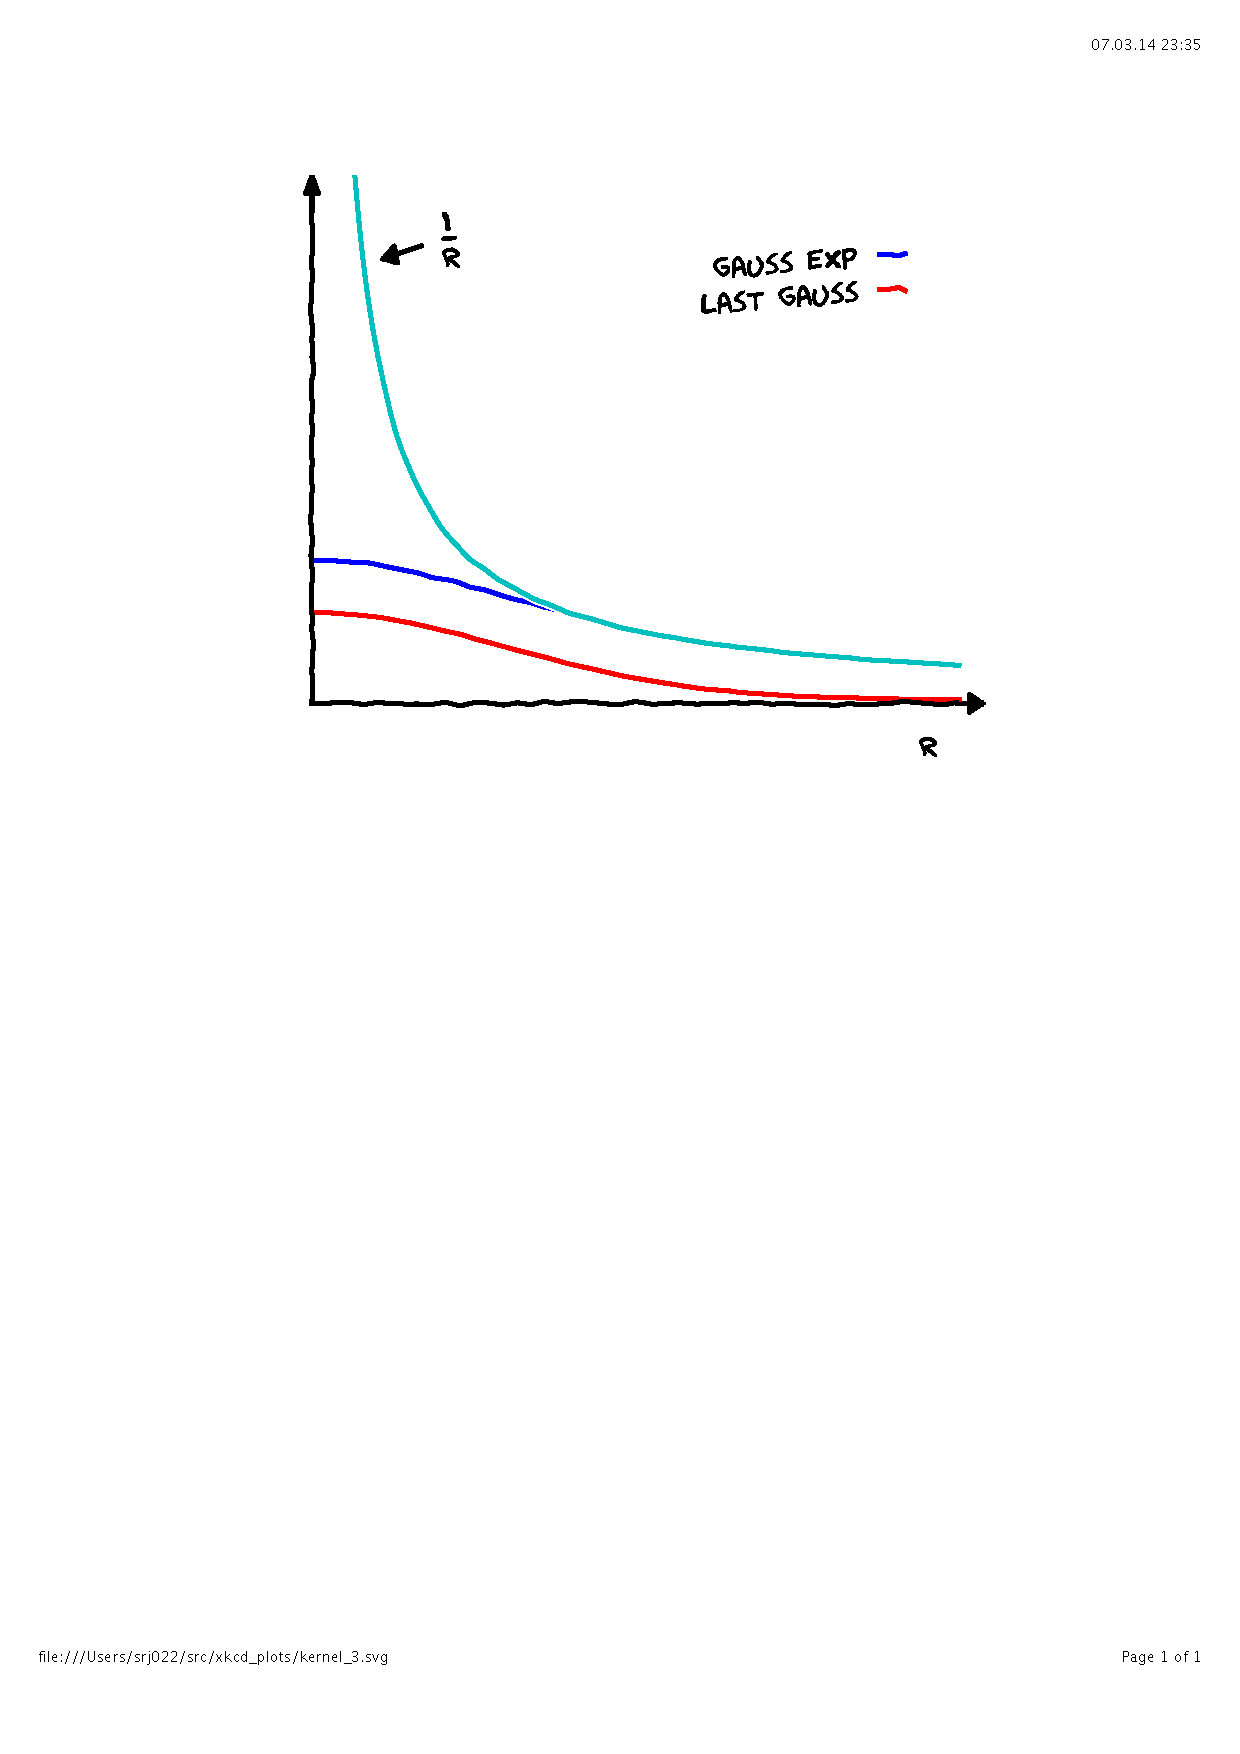
\includegraphics[scale=0.5, clip, viewport = 110 450 490 800]{figures/kernel_3.pdf}}
	\only<4>{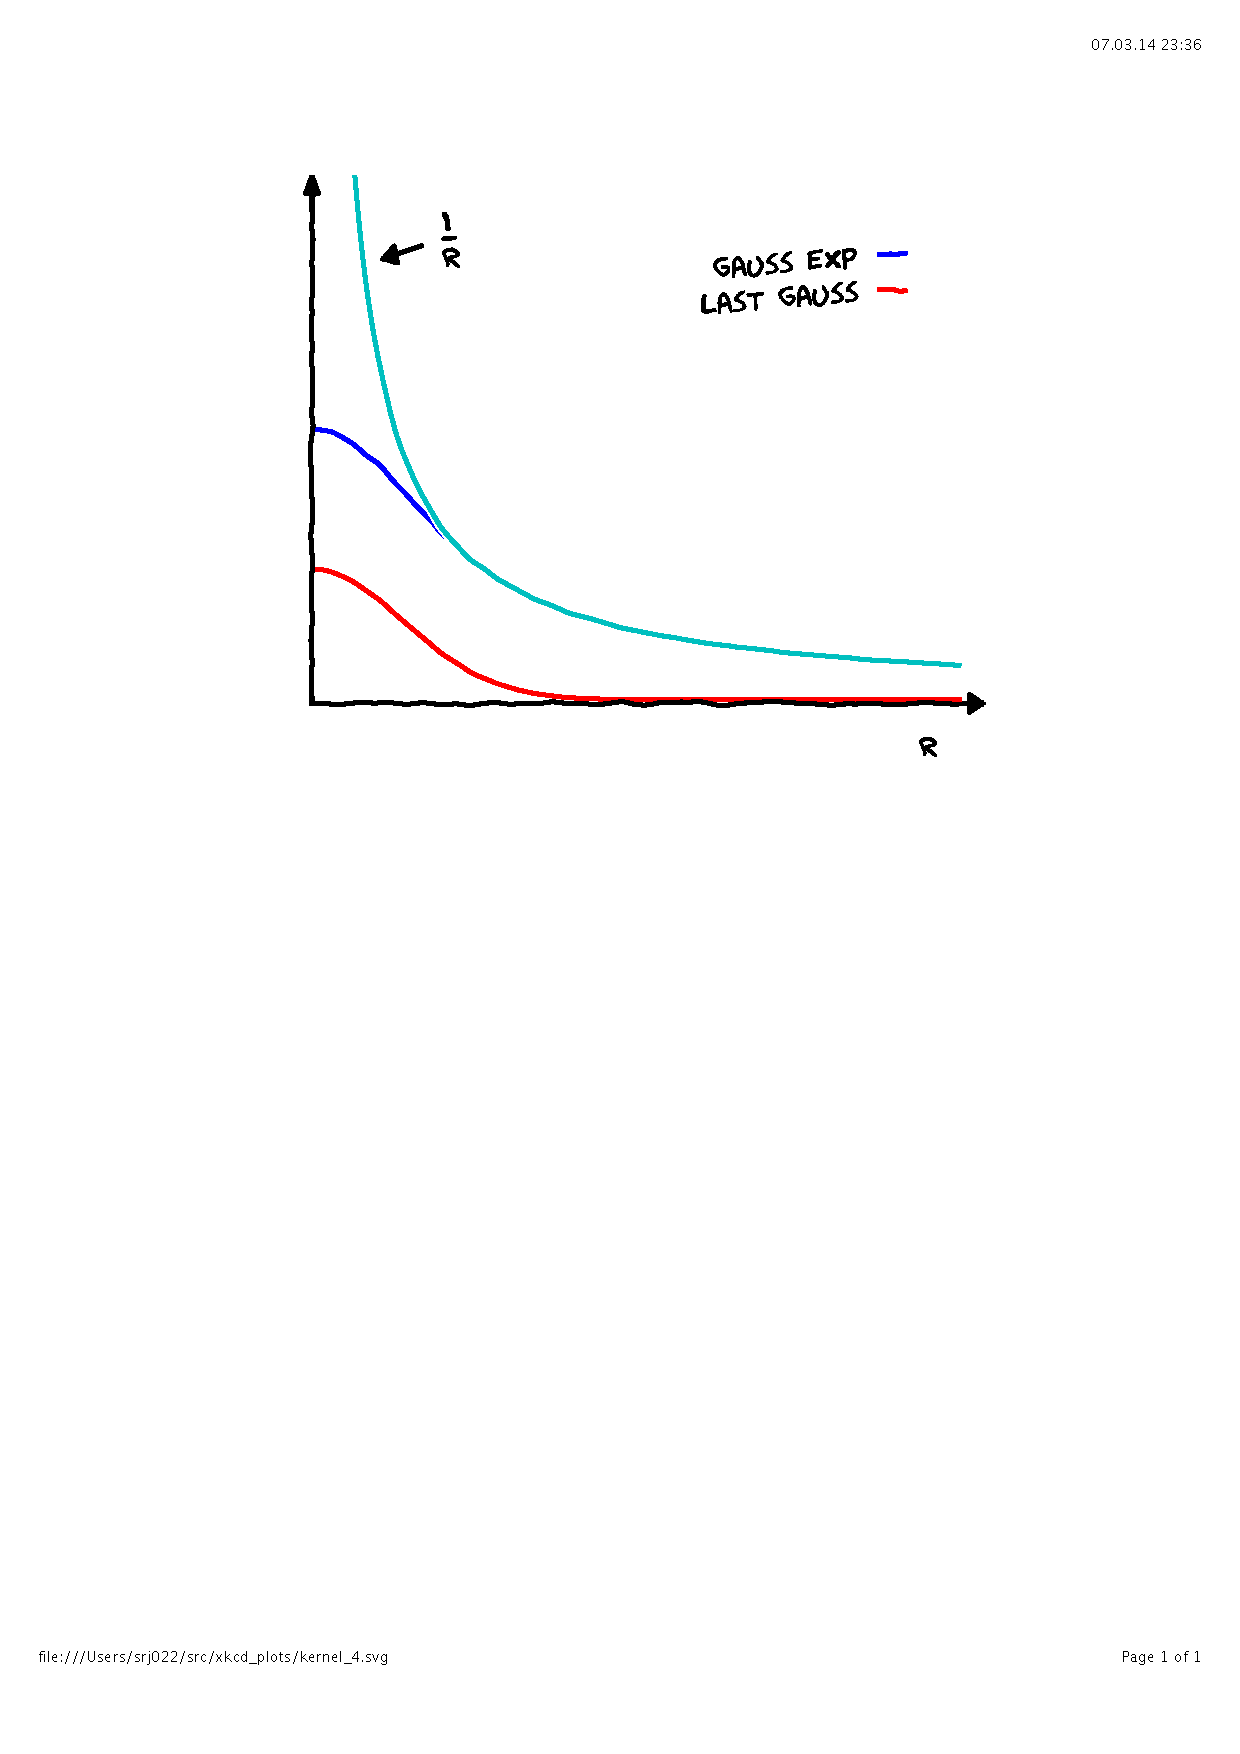
\includegraphics[scale=0.5, clip, viewport = 110 450 490 800]{figures/kernel_4.pdf}}
	\only<5>{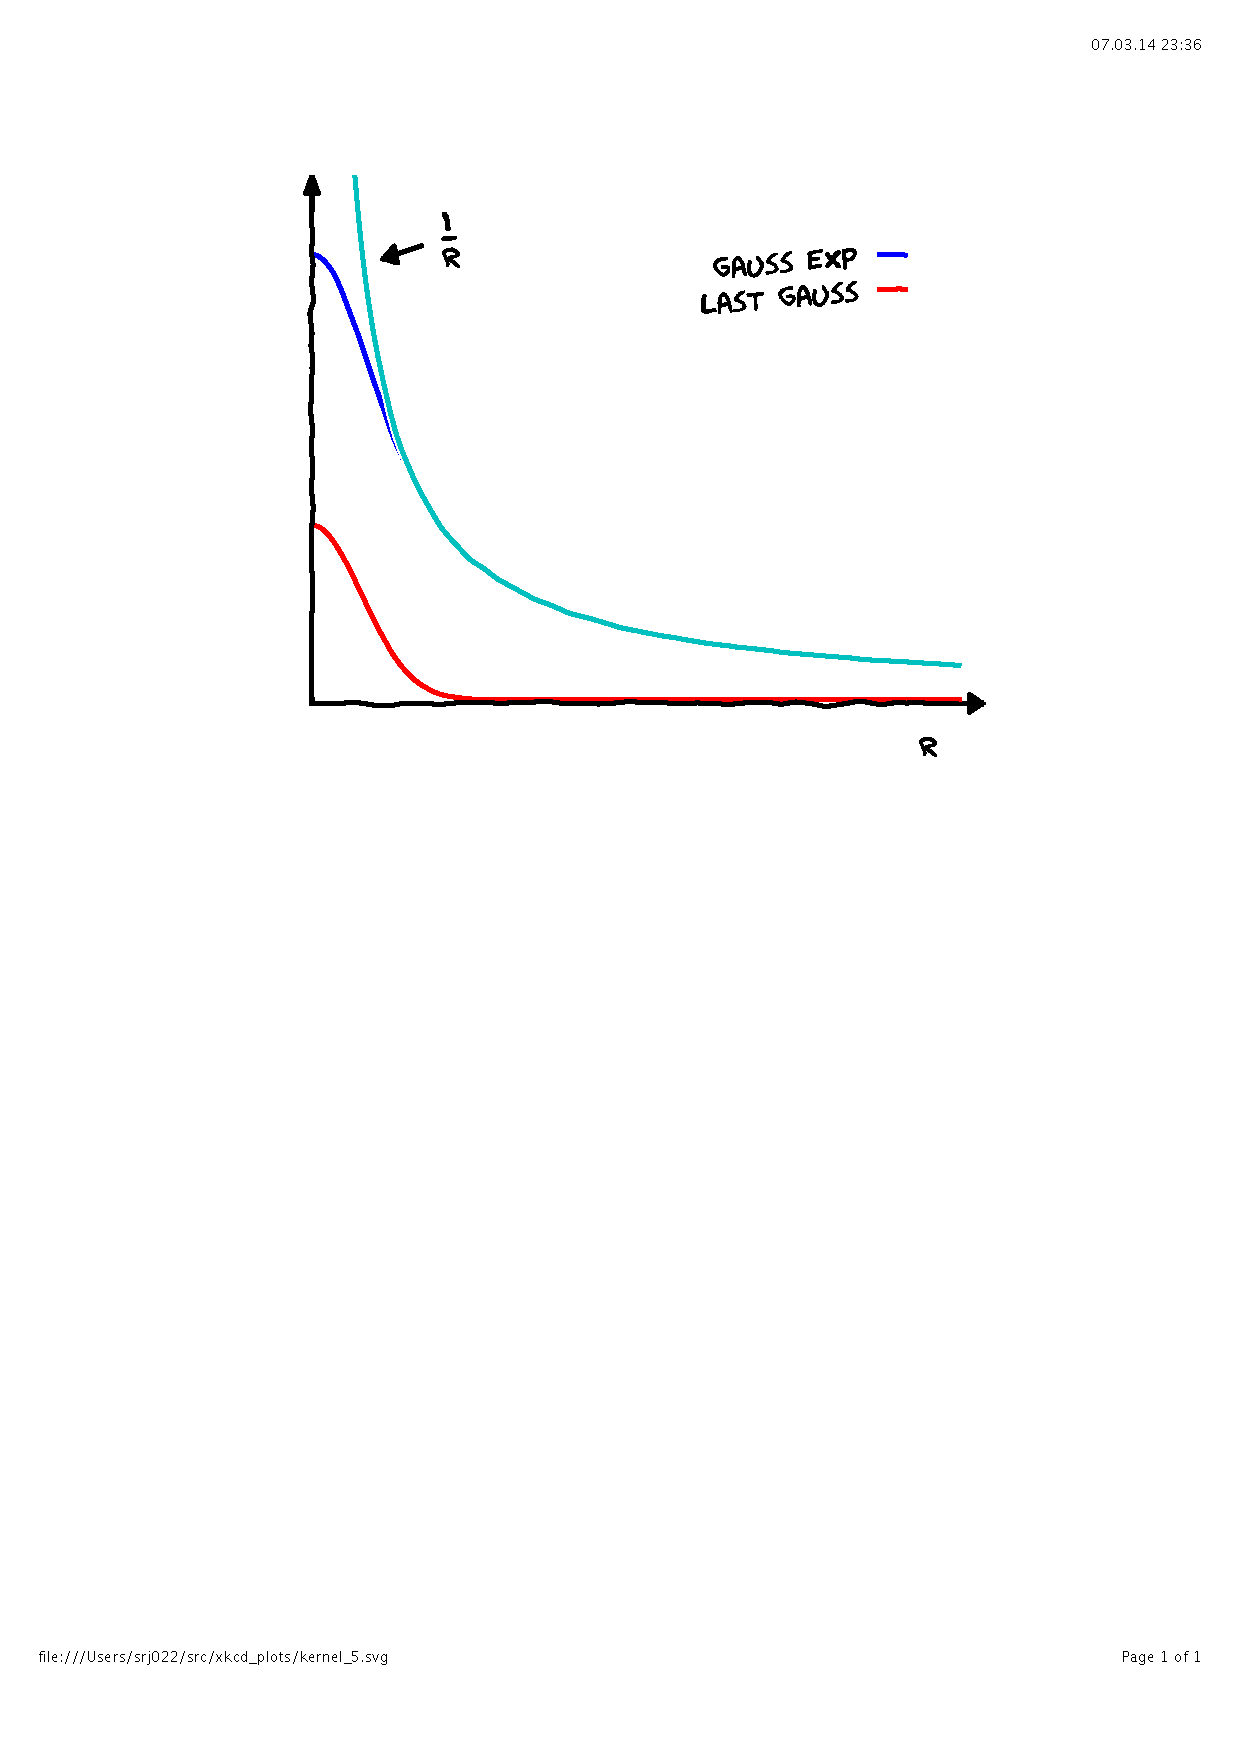
\includegraphics[scale=0.5, clip, viewport = 110 450 490 800]{figures/kernel_5.pdf}}
	\only<6>{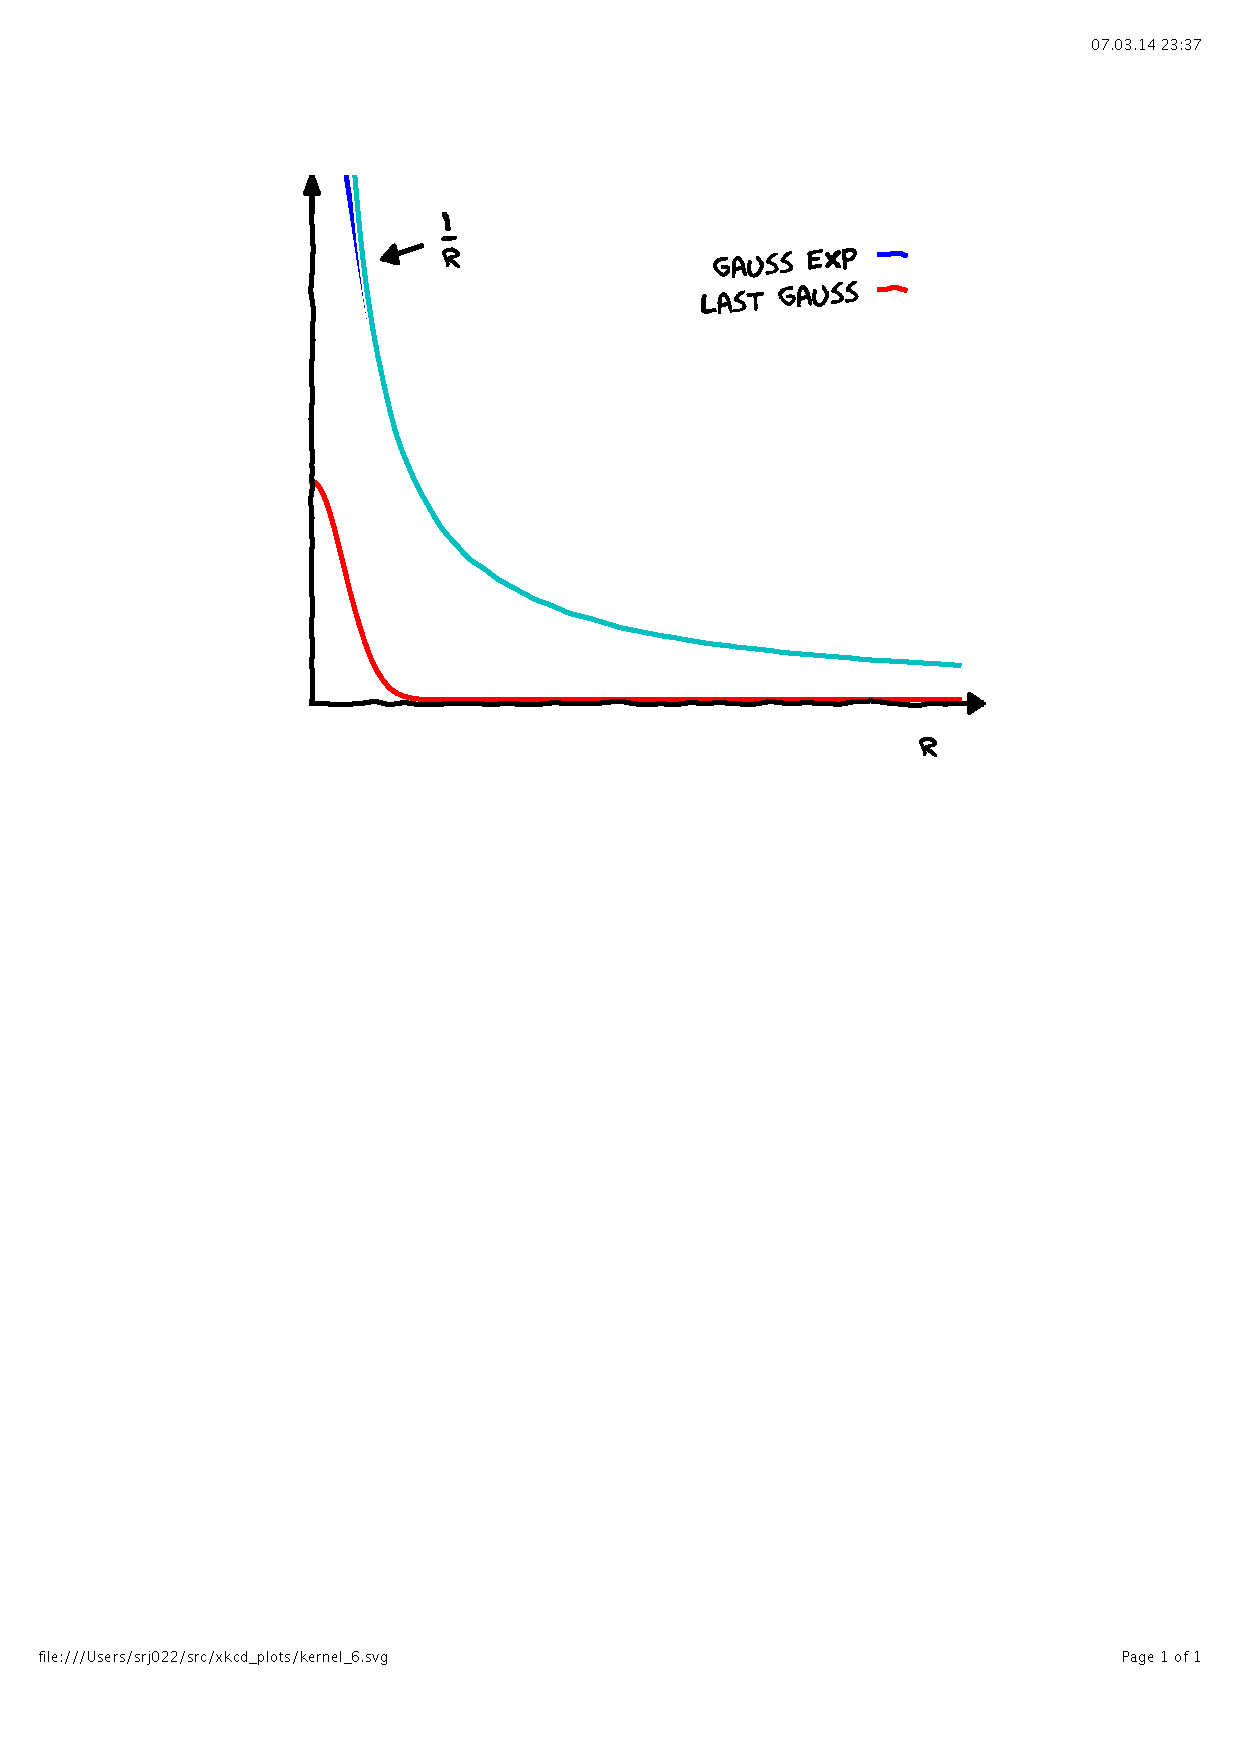
\includegraphics[scale=0.5, clip, viewport = 110 450 490 800]{figures/kernel_6.pdf}}
	\only<7>{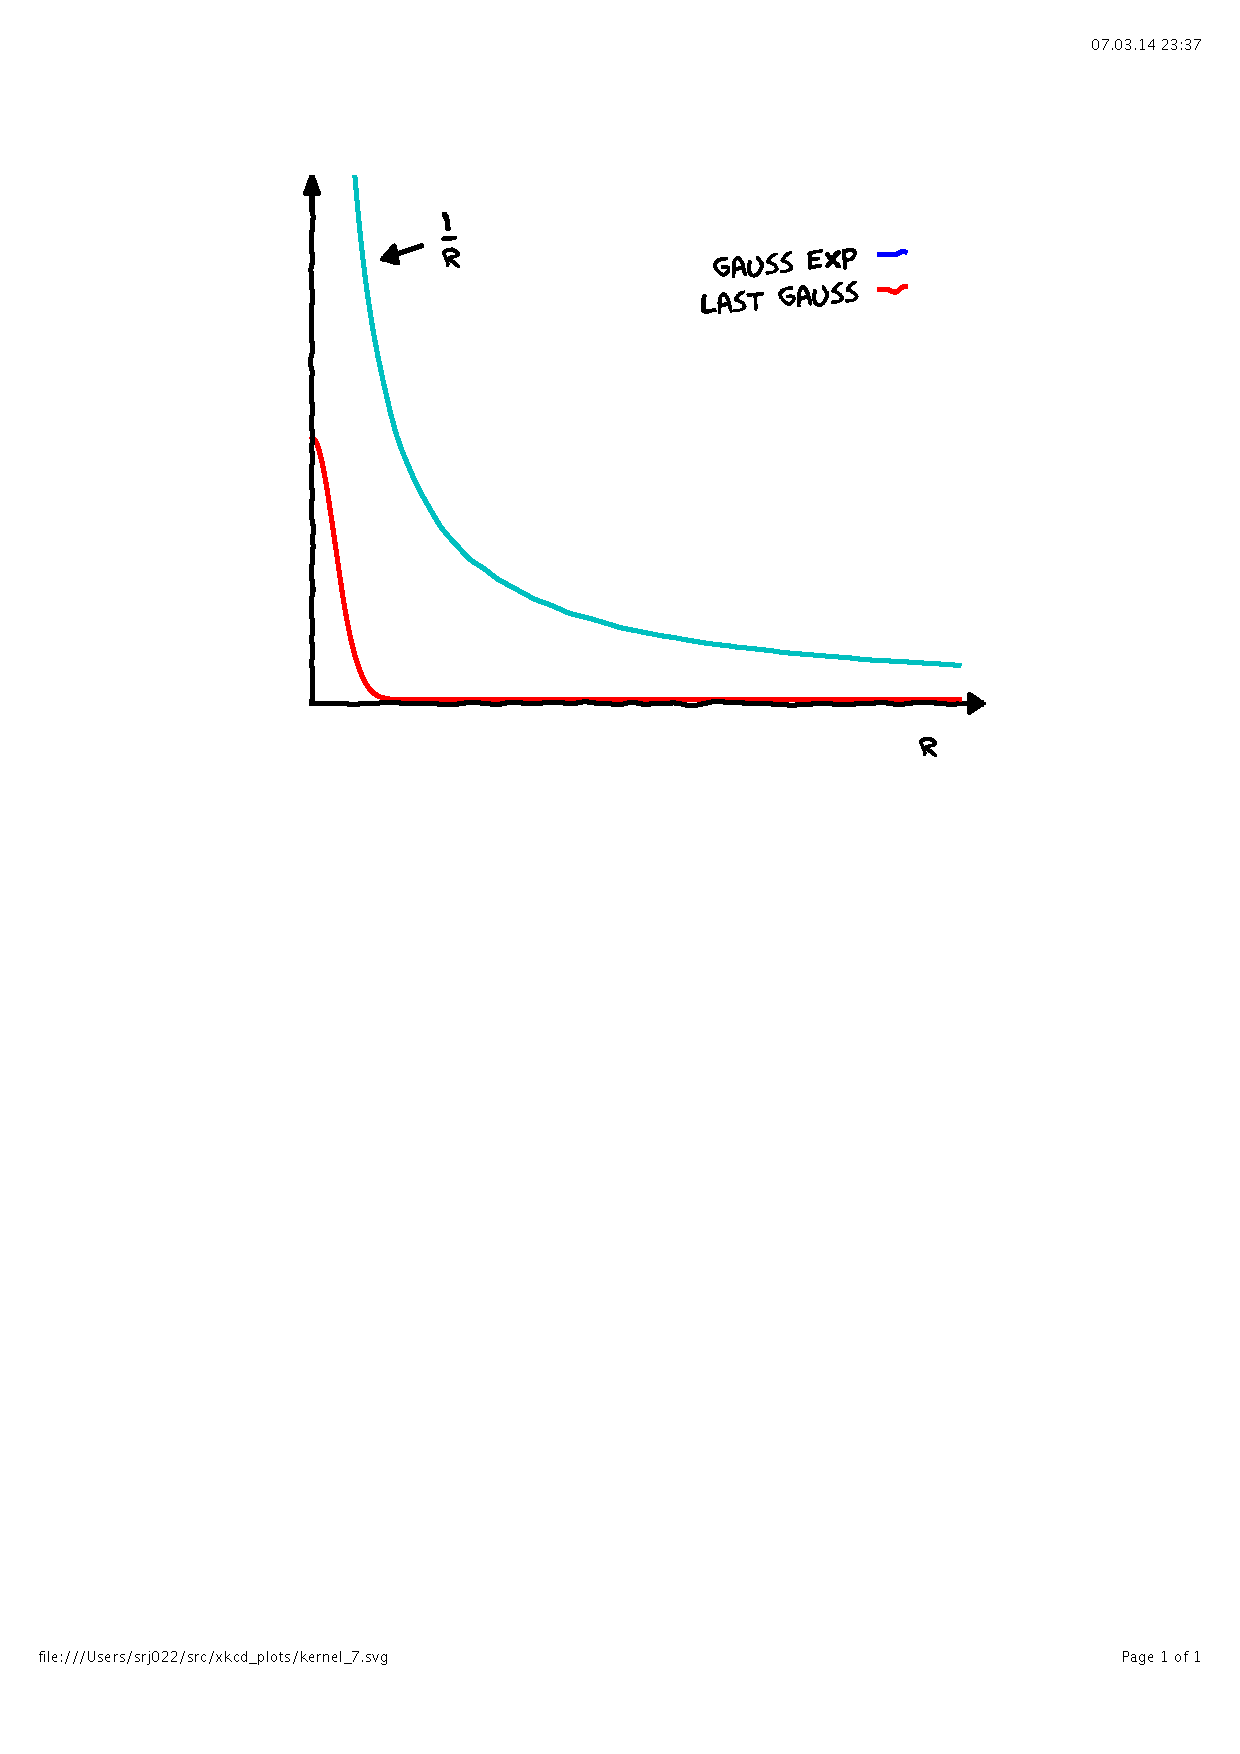
\includegraphics[scale=0.5, clip, viewport = 110 450 490 800]{figures/kernel_7.pdf}}
    \end{column}
    \end{columns}    
\end{frame}

\begin{frame}
    \frametitle{Vanishing moments}
    A function $\psi(x)$ is said to have M vanishing moments if
    \begin{equation}
	\nonumber
        \mu_m = \int_0^1 x^m\psi(x) dx = 0 \ \ \ \ \ \ \ \ \ \ \ m = 0,1,\dots,M-1 
    \end{equation}
    \ \\
    \ \\
    \begin{center}
	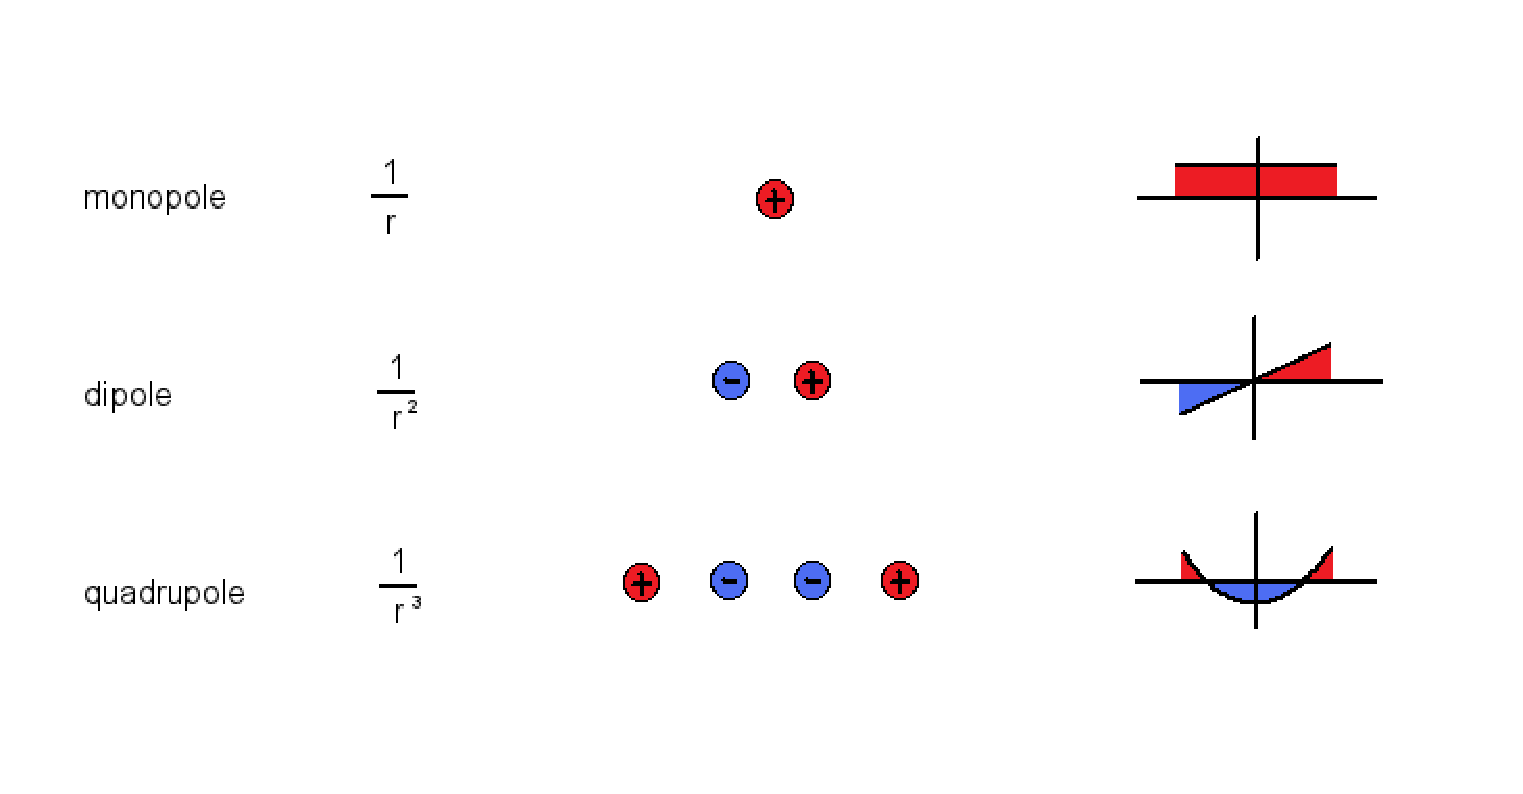
\includegraphics[scale=0.4, clip, viewport = 0 50 700 350]{figures/multipoles.pdf}
    \end{center}
\end{frame}

\begin{frame}
    \frametitle{Operators in Non-Standard form}
    \tiny
    \only<1>{
    \begin{equation}
	\nonumber
	T^N \textcolor{white}{= T^{N-1} + \Bigg[C^{N-1}+B^{N-1}+A^{N-1}\Bigg]}
    \end{equation}}
    \only<2,3>{
    \begin{equation}
	\nonumber
	T^N = T^{N-1} + \Bigg[C^{N-1}+B^{N-1}+A^{N-1}\Bigg]
    \end{equation}}
    \only<4,5>{
    \begin{equation}
	\nonumber
	T^N = T^{N-2} + \Bigg[C^{N-2}+B^{N-2}+A^{N-2}\Bigg] + \Bigg[C^{N-1}+B^{N-1}+A^{N-1}\Bigg]
    \end{equation}}
    \only<6>{
    \begin{equation}
	\nonumber
	T^N = T^0 + \sum_{n=0}^{N-1} \Bigg[C^n+B^n+A^n\Bigg]
    \end{equation}}
    \begin{center}
    \only<1>{
\includegraphics[scale=0.8, clip, viewport = 240 280 450 480]{figures/matrix/matrix_1.pdf}}
    \only<2>{
\includegraphics[scale=0.8, clip, viewport = 240 280 450 480]{figures/matrix/matrix_2.pdf}}
    \only<3>{
\includegraphics[scale=0.8, clip, viewport = 240 280 450 480]{figures/matrix/matrix_3.pdf}}
    \only<4>{
\includegraphics[scale=0.8, clip, viewport = 240 280 450 480]{figures/matrix/matrix_4.pdf}}
    \only<5>{
\includegraphics[scale=0.8, clip, viewport = 240 280 450 480]{figures/matrix/matrix_5.pdf}}
    \only<6>{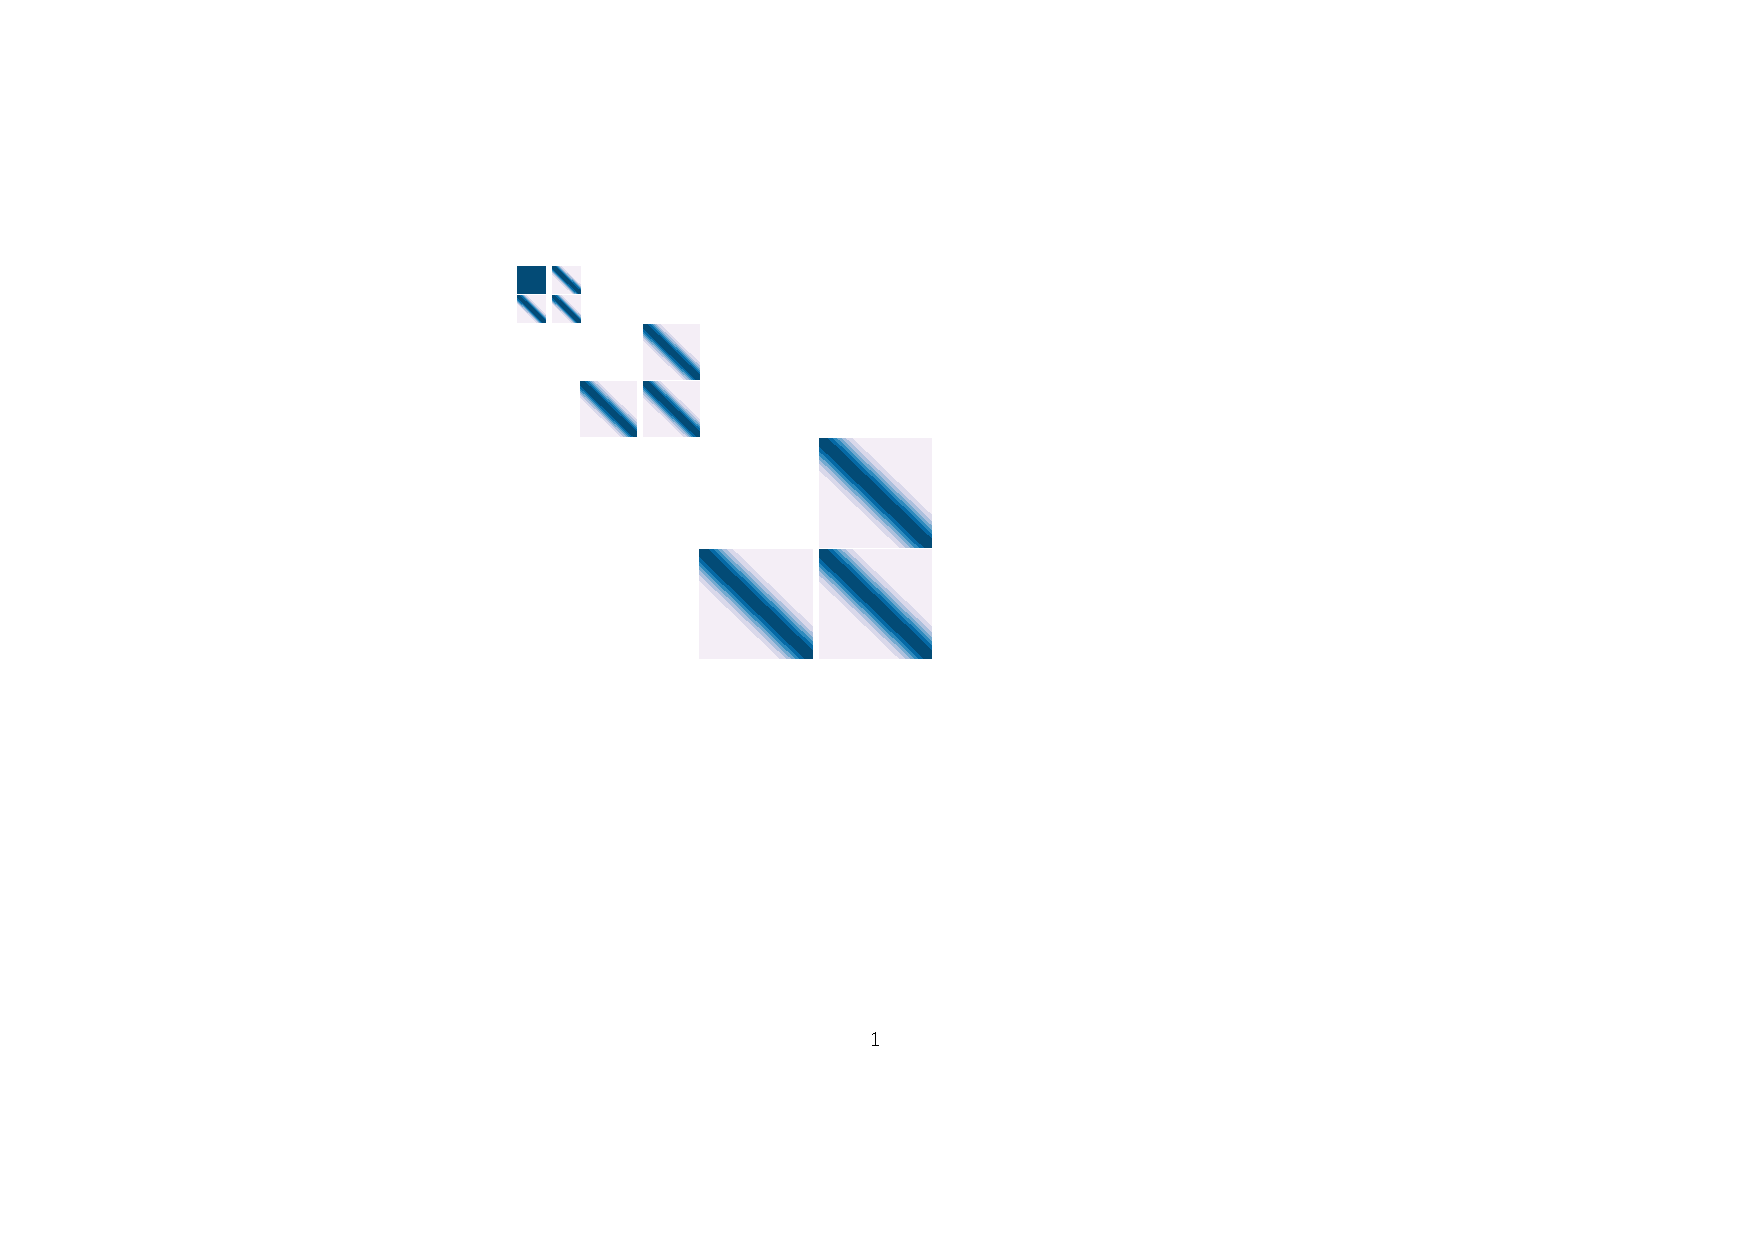
\includegraphics[scale=0.8, clip, viewport = 240 280 450 480]{figures/matrix/matrix_6.pdf}}
    \end{center}
\end{frame}

\begin{frame}
    \frametitle{Linear scaling Coulomb interaction}
    \begin{columns}
    \begin{column}{.40\textwidth}
    Alkane chains
    \begin{equation}
	\nonumber
	C_{n}H_{2n+2}, \qquad n=2,\dots,70
    \end{equation}
    \end{column}
    \begin{column}{.60\textwidth}
	\begin{figure}
	    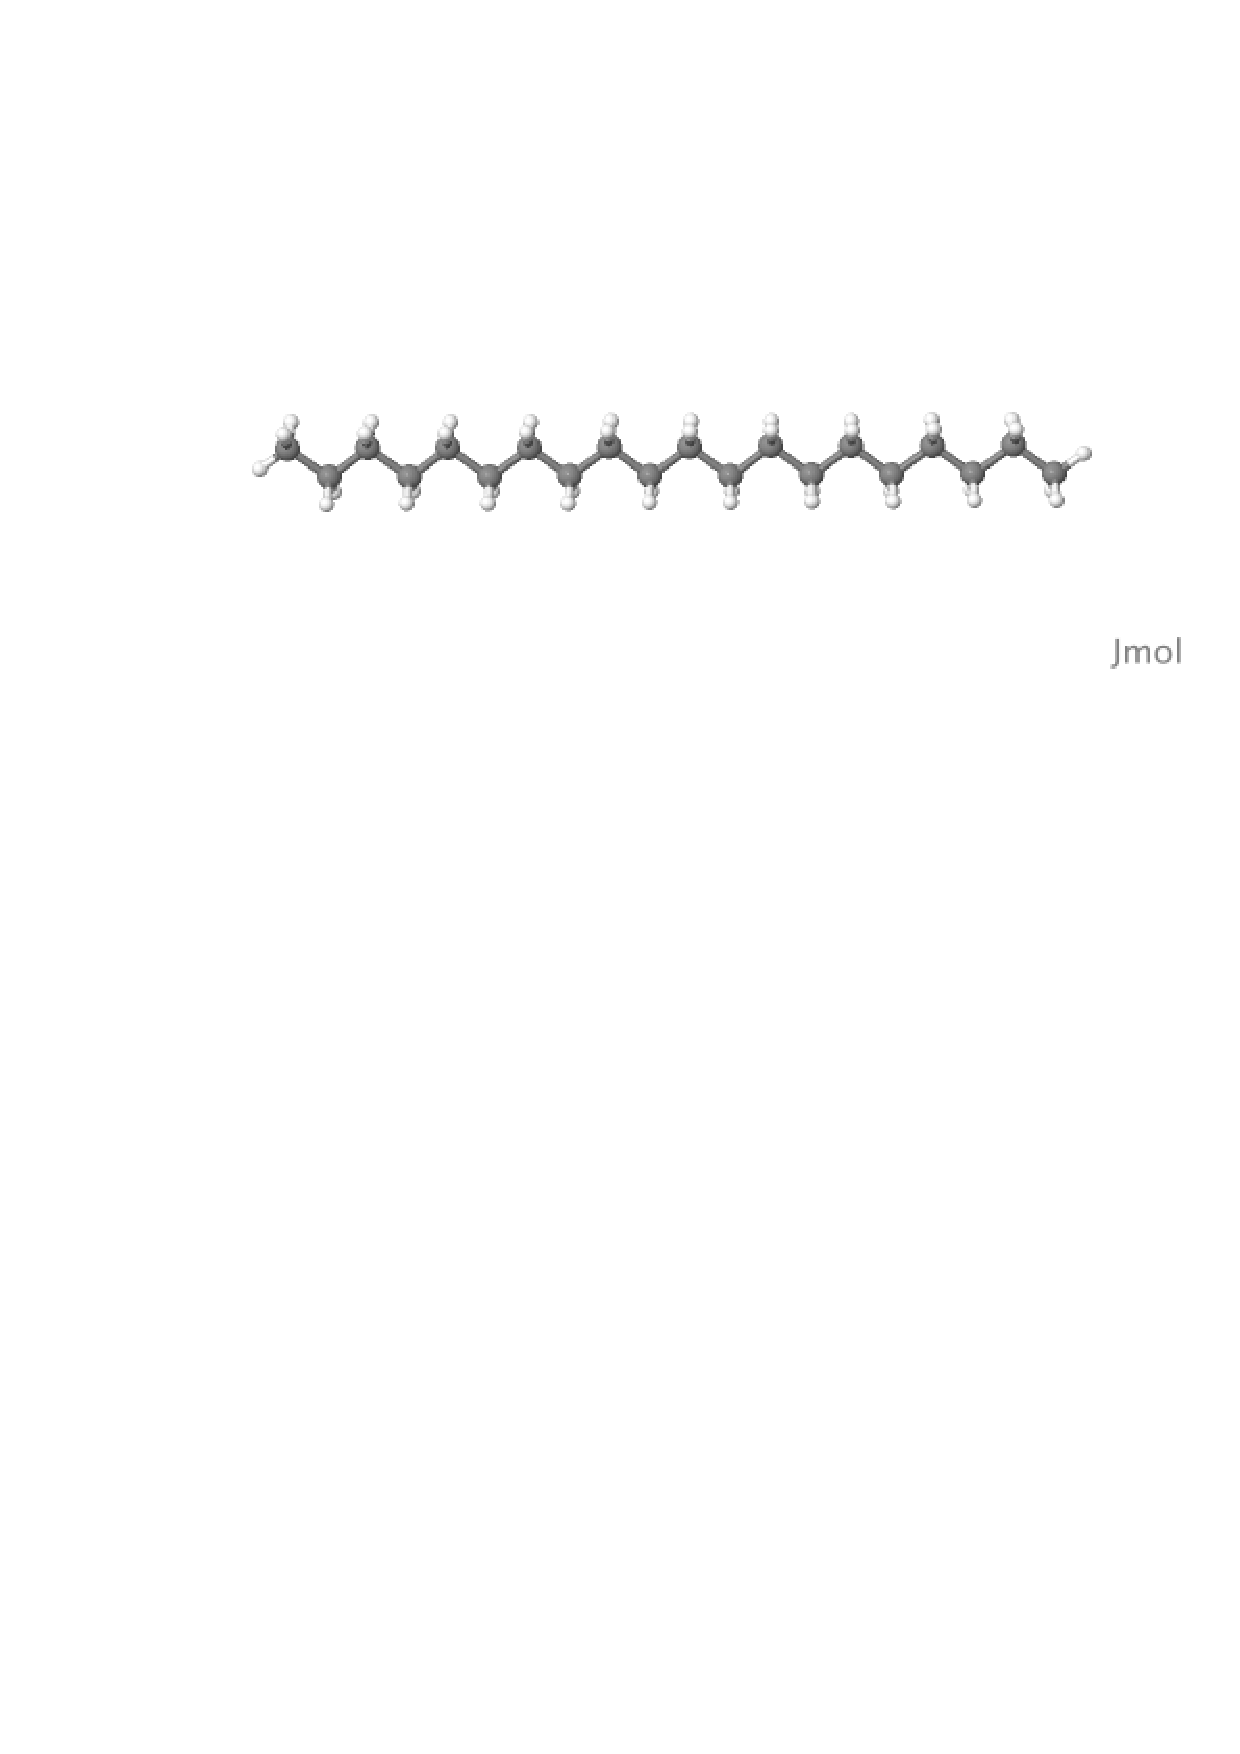
\includegraphics[scale=0.3, clip, viewport = 80 560 600 720]{figures/alkane.pdf}
	\end{figure}
    \end{column}
    \end{columns}    
    \ \\
    Best fit curves
    \begin{equation}
	\nonumber
	T(N) = 12.5 + 2.34N^{0.754} \qquad \qquad \qquad T(N) = -6.0 + 1.33N^{0.991}
    \end{equation}
    \ \\
    \begin{center}
	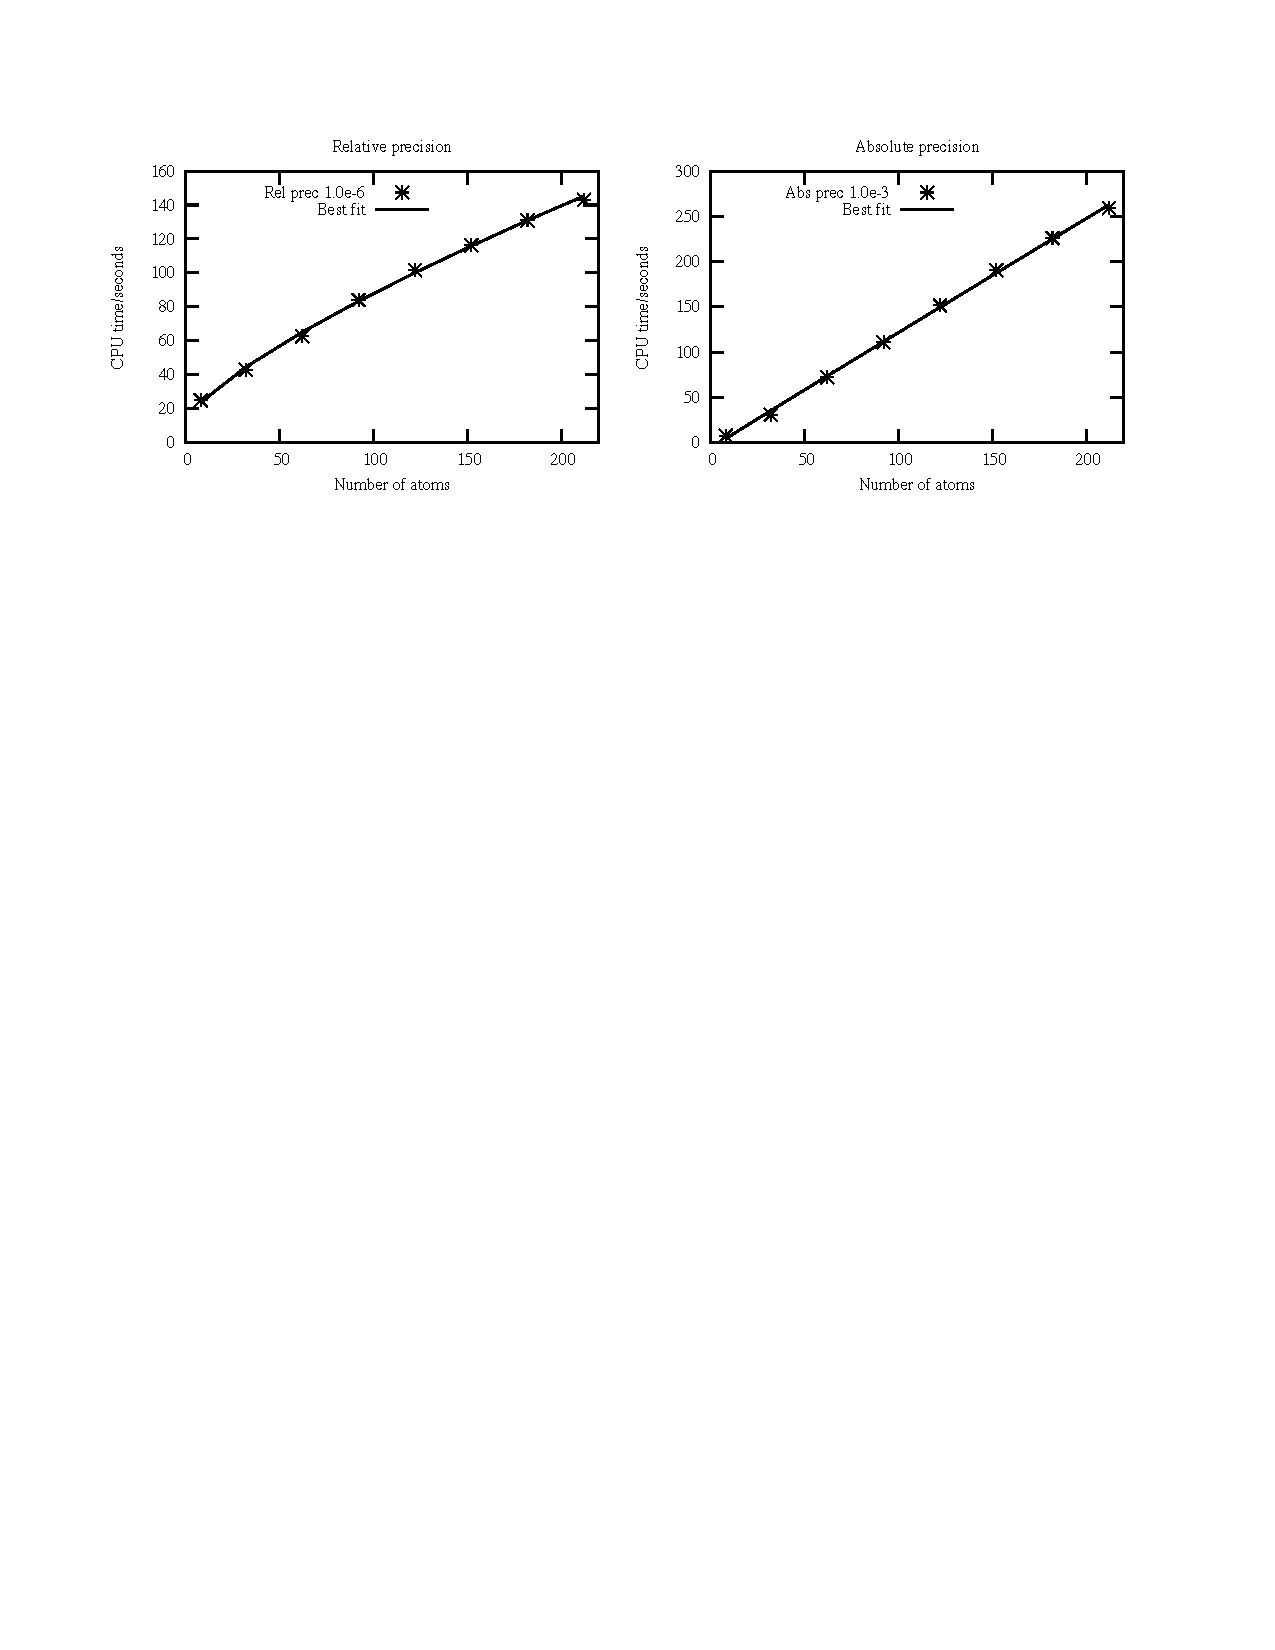
\includegraphics[scale=0.6, clip, viewport = 50 550 540 730]{figures/linearScaling.pdf}
    \end{center}
\end{frame}

\begin{frame}
    \frametitle{Parallel performance OpenMP}
    \begin{columns}
    \begin{column}{.50\textwidth}
    Diamond fragments $n=1,\dots,9$
    \begin{equation}
	\nonumber
	C_{(2n+3)(n+2)(n+1)/6}H_{2(n+2)(n+1)}
    \end{equation}
    \ \\
    \ \\
    Best fit curve
    \begin{equation}
	\nonumber
	T(N) = 11.6 + 1.84N^{0.805} \qquad\qquad\qquad\qquad\qquad\qquad\qquad\qquad
    \end{equation}
    \end{column}
    \begin{column}{.50\textwidth}
	\begin{figure}
	    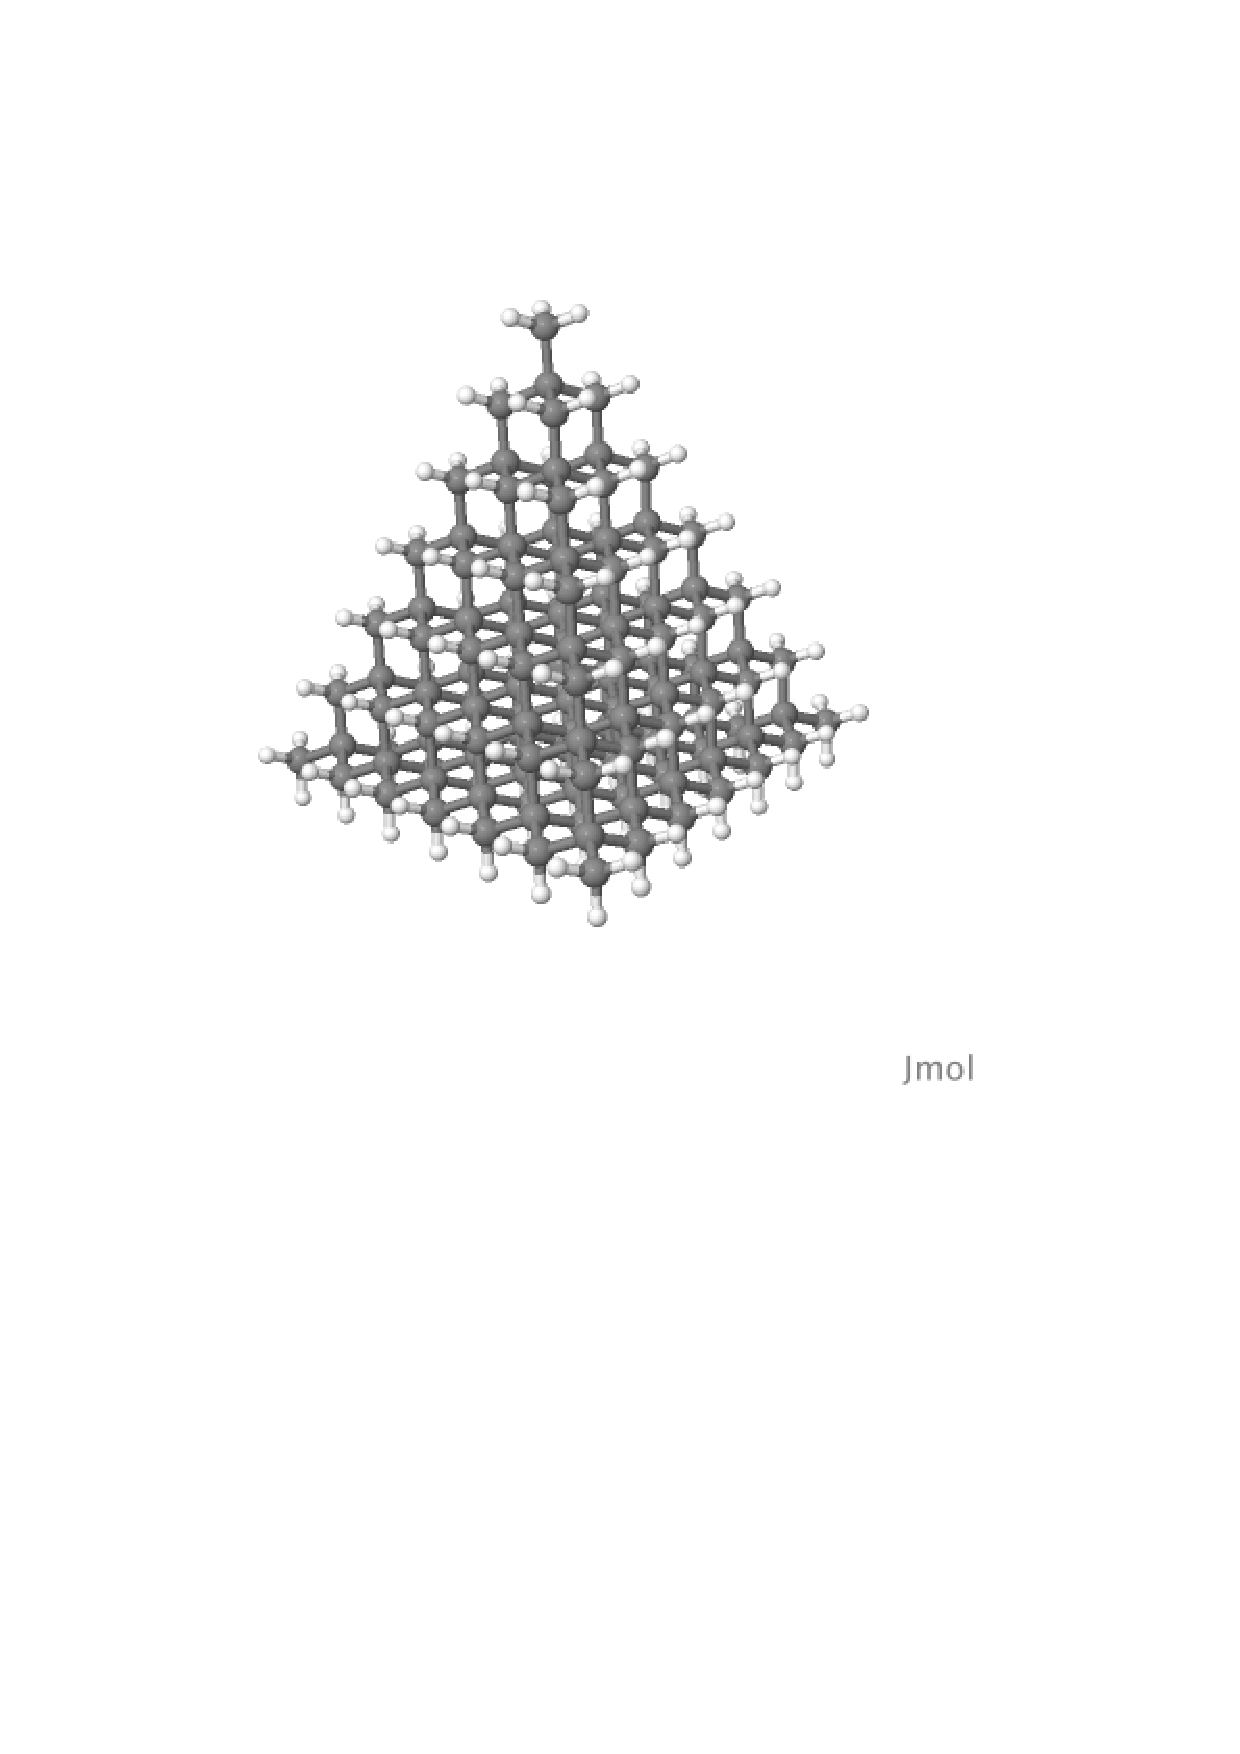
\includegraphics[scale=0.25, clip, viewport = 10 390 500 720]{figures/diamond.pdf}
	\end{figure}
    \end{column}
    \end{columns}    
    \ \\
    \begin{center}
	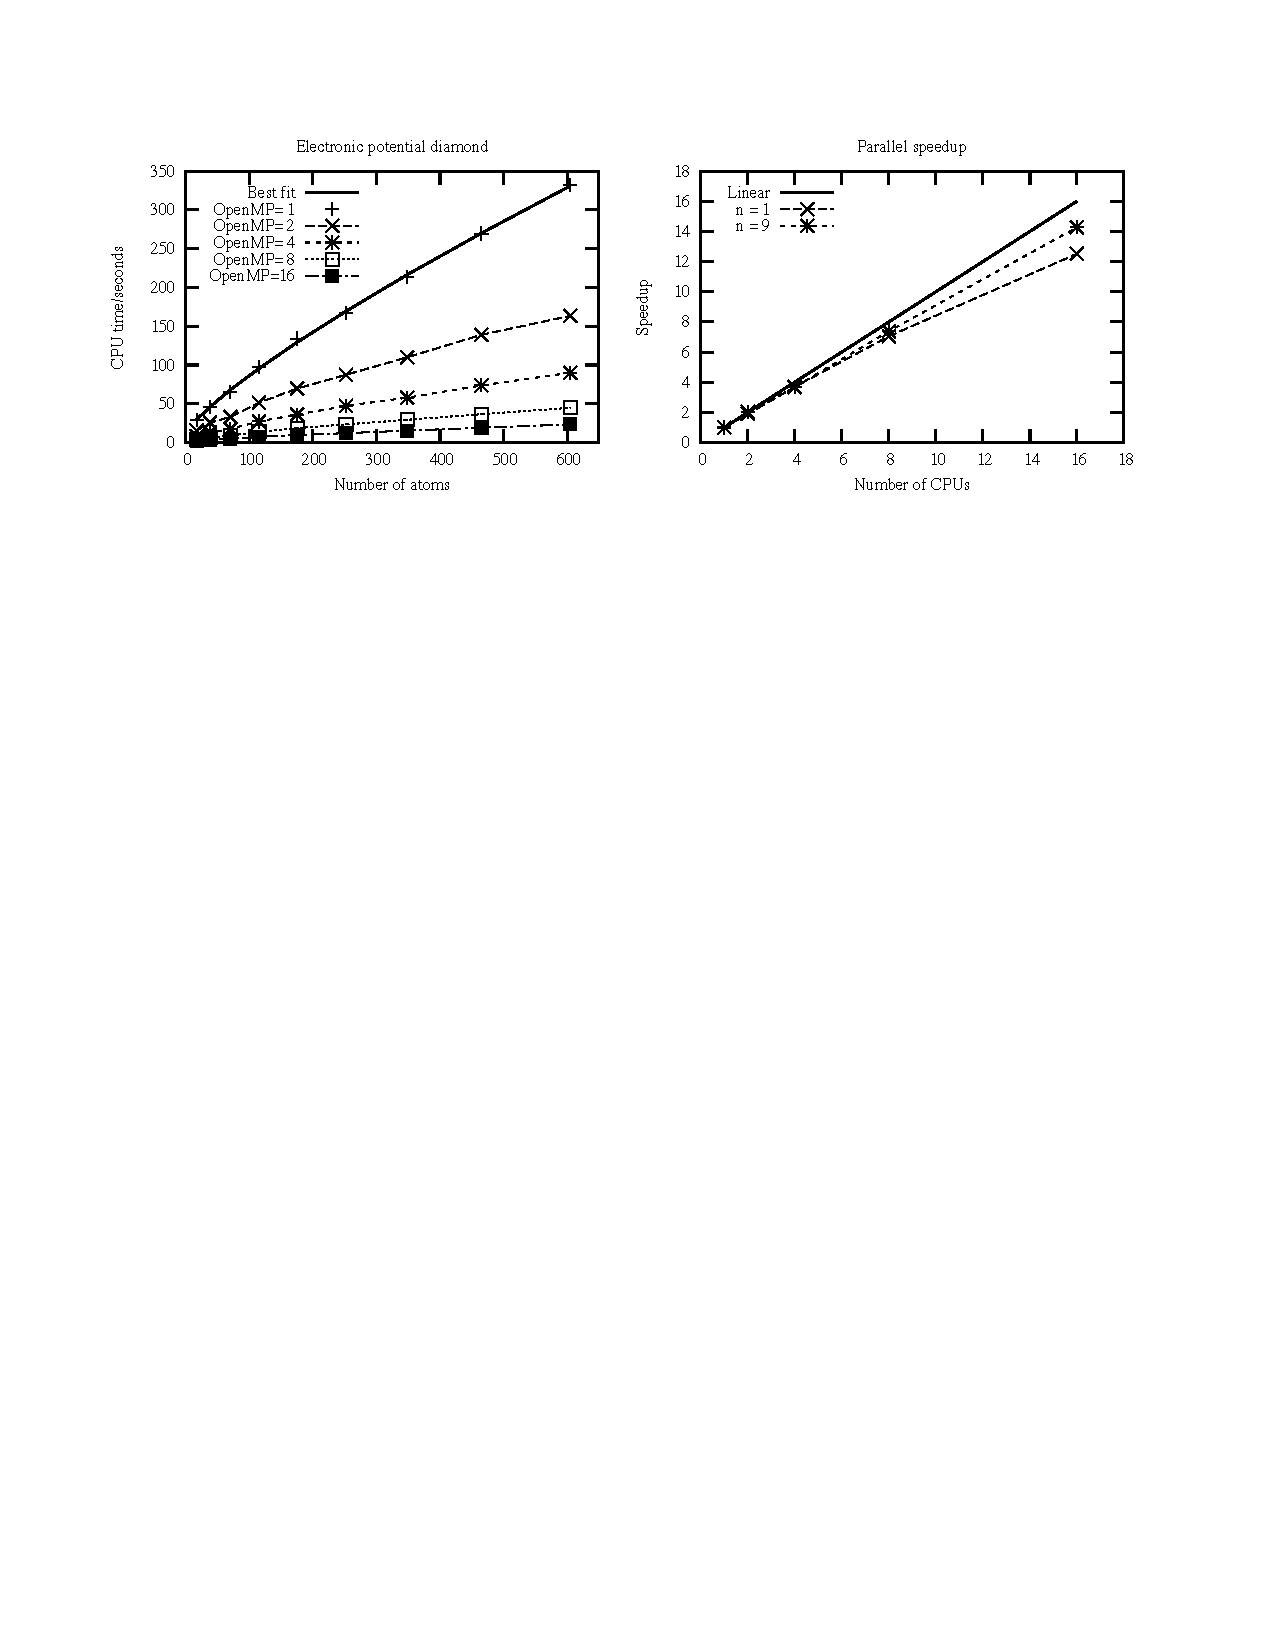
\includegraphics[scale=0.6, clip, viewport = 50 550 540 730]{figures/ompScaling.pdf}
    \end{center}
\end{frame}

\begin{frame}
    \frametitle{Parallel performance MPI}
    \begin{table}
    \tiny
    \centering
    \caption{\scriptsize{Wall clock computation time in seconds for parallel calculation of 
	electronic potential of diamond fragments using pure OpenMP, pure MPI and hybrid 
	MPI/OpenMP strategies.}}
    \begin{tabular}{cccrrrrrrrrr}
	\hline
	\hline                                                                           
	\multicolumn{3}{c}{Number of CPUs}&
	\multicolumn{9}{c}{Diamond system $n$ in $C_{(2n+3)(n+2)(n+1)/6}H_{2(n+2)(n+1)}$}\\
	MPI&OMP&TOT	&1	&2	&3	&4	&5	&6	&7	&8	&9	\\
	\hline
	   &   &   	&	&      	&	&	&	&	&	&	&	\\
	  1&  1&  1	& 29.4	& 46.2 	& 64.7 	& 97.8  &133.9  &166.8  &213.4  &269.4  &332.0  \\
	  1&  2&  2	& 15.5	& 25.5 	& 33.0 	& 51.3  & 69.5  & 87.2  &110.0  &138.9  &163.4  \\
	  1&  4&  4	&  8.0 	& 12.8 	& 17.4 	& 27.0  & 36.1  & 47.3  & 57.8  & 73.7  & 90.1  \\
	  1&  8&  8	&  4.2 	&  6.5 	&  8.8 	& 13.9  & 18.6  & 23.5  & 29.4  & 36.7  & 45.0  \\
	  1& 16& 16	&  2.4 	&  3.5 	&  4.7 	&  7.5  &  9.6  & 12.2  & 15.4  & 19.1  & 23.3  \\
	   &   &   	&      	&      	&    	&    	&    	&	&	&	&	\\
	  2&  1&  2	& 17.9 	& 28.4 	& 35.8 	& 59.2  & 81.6  & 93.0  &121.7  &147.5  &176.5  \\
	  4&  1&  4	& 10.1 	& 16.3 	& 21.2 	& 32.5  & 51.6  & 53.8  & 60.8  & 85.3  &100.7  \\
	  8&  1&  8	&  6.1 	&  9.4 	& 11.8 	& 19.9  & 25.6  & 28.0  & 35.4  & 43.7  & 50.7  \\
	 16&  1& 16	&  5.0 	&  6.2 	&  8.2 	& 12.4  & 15.0  & 17.3  & 23.0  & 26.1  & 31.3  \\
	 32&  1& 32	&  3.6 	&  4.2 	&  5.4 	&  9.5  &  9.2  & 10.9  & 14.1  & 16.8  & 20.0  \\
	 64&  1& 64	&  3.1 	&  3.9 	&  4.3 	&  6.5  &  6.6  &  7.4  & 10.3  & 11.4  & 13.4  \\
	128&  1&128	&  5.2 	&  5.7 	&  6.4 	&  7.6  &  7.8  &  8.8  & 10.9  & 10.9  & 11.9  \\
	   &   &   	&      	&      	&      	& 	& 	& 	& 	& 	&	\\
	  2& 16& 32	&  1.5 	&  2.2 	&  2.9 	&  4.8  &  6.0  &  7.0  &  9.6  & 11.4  & 13.7  \\
	  4& 16& 64	&  1.1 	&  1.6 	&  2.0 	&  3.2  &  4.3  &  4.7  &  6.3  &  7.3  &  7.9  \\
	  8& 16&128	&  1.0 	&  1.4 	&  1.8 	&  2.9  &  3.3  &  3.8  &  4.8  &  5.9  &  6.4  \\
	 16& 16&256	&  0.9 	&  1.3 	&  1.6 	&  2.2  &  2.9  &  3.3  &  4.2  &  4.9  &  6.0  \\
	 32& 16&512	&  1.1 	&  1.3 	&  1.5 	&  2.0  &  2.4  &  2.8  &  3.4  &  4.0  &  4.8  \\
	   &   &   	&      	&      	&      	&    	&    	&	&	&	&	\\
	\hline                                                                           
	\hline
    \end{tabular}
    \end{table}
\end{frame}

\begin{frame}
    \frametitle{The molecular Schr\"{o}dinger equation}
    \ \\
    \begin{equation}
	\nonumber
	\hat{H}\psi = E\psi
    \end{equation}
    \ \\
    \begin{equation}
	\nonumber
	\hat{H} =   -\sum_I \frac{\nabla^2}{2M_I} - \sum_i \frac{\nabla^2}{2}
		    +\sum_{I>J} \frac{Z_IZ_J}{|\boldsymbol{R}_I-\boldsymbol{R}_J|} 
		    -\sum_{i,I} \frac{Z_I}{|\boldsymbol{r}_i-\boldsymbol{R}_I|} 
		    +\sum_{i>j} \frac{1}{|\boldsymbol{r}_i-\boldsymbol{r}_j|} 
    \end{equation}
    \ \\
    \ \\
    \ \\
    For an $N$-particle problem, the wave function is $3N$-dimensional
    \begin{equation}
	\nonumber
	\psi = \psi(\boldsymbol{r}_1,\boldsymbol{r}_2,\dots,\boldsymbol{r}_N)
    \end{equation}
    \ \\
    \ \\
    \ \\
    \pause
    $\beta$-Carotene ($C_{40}H_{56}$) has 296 electrons and an 888-dimensional wave function!
    \only<1>{
    \begin{center}
    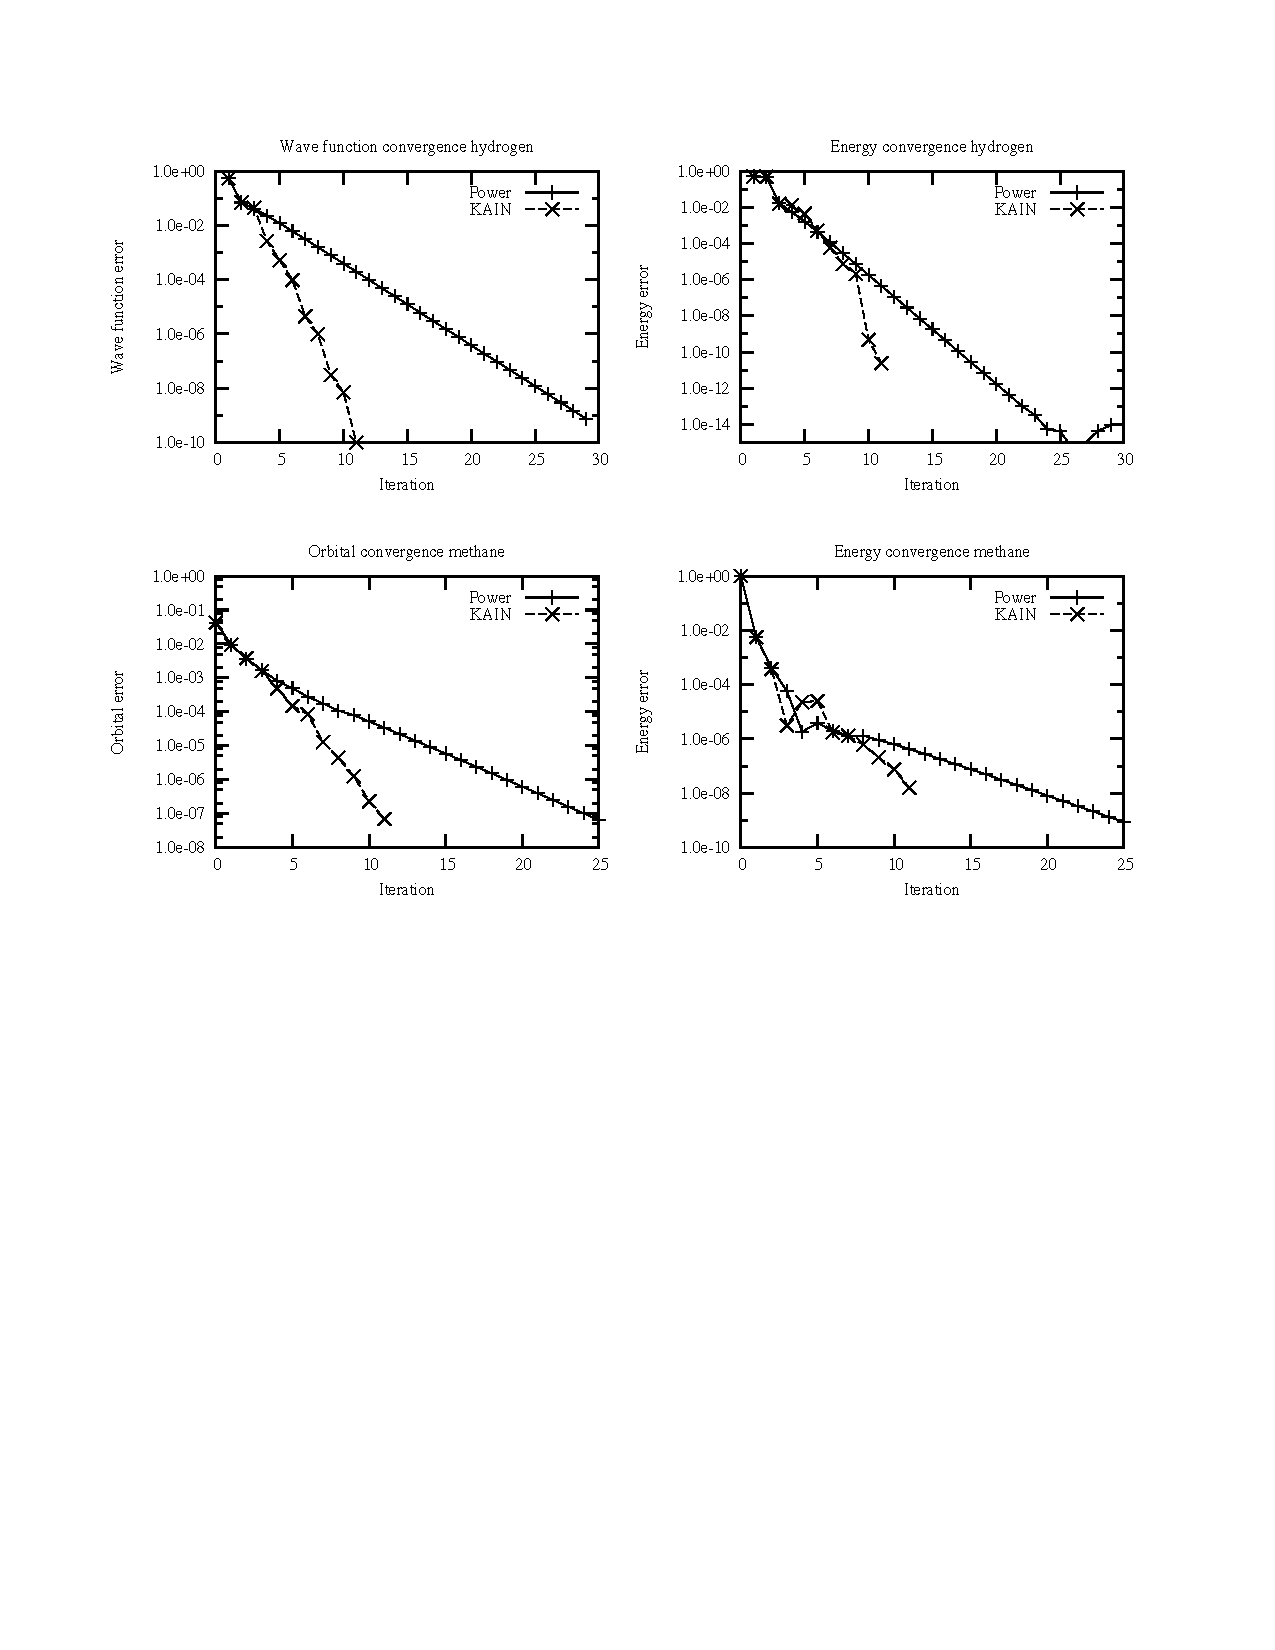
\includegraphics[scale=0.3, clip, viewport = 0 0 900 280]{figures/convergence.pdf}
    \end{center}
    }
    \only<2>{
    \begin{center}
    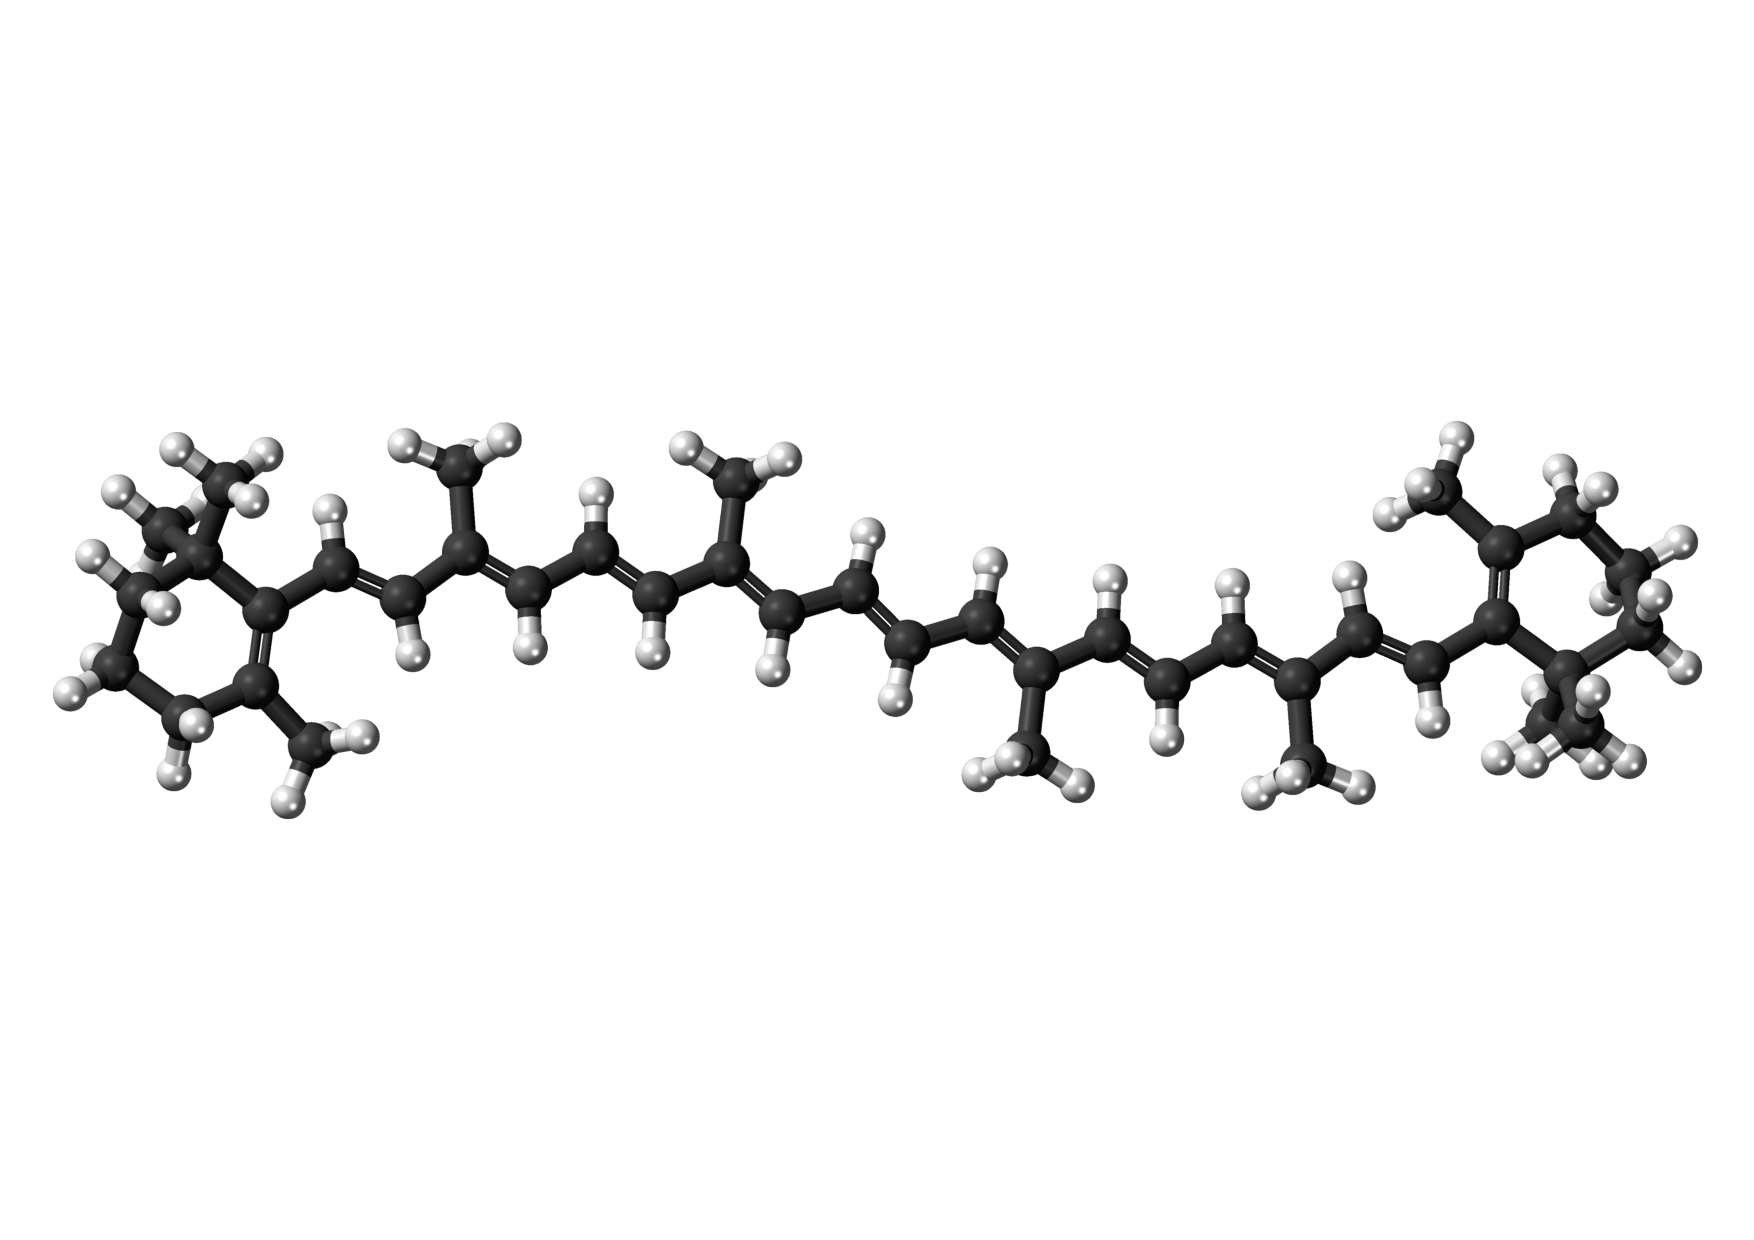
\includegraphics[scale=0.3, clip, viewport = 0 150 900 430]{figures/beta-carotene.pdf}
    \end{center}
    }
\end{frame}

\begin{frame}
    \frametitle{Density Functional Theory}
    Dramatically reduce the dimensionality 
    \begin{equation}
	\rho(\boldsymbol{r}_1) = N \int |\psi(\boldsymbol{r}_1, \boldsymbol{r}_2,\dots,
	\boldsymbol{r}_N)|^2 d\boldsymbol{r}_2\cdots d\boldsymbol{r}_N
    \end{equation}
    and the energy is expressed in terms of the electron density 
    \begin{equation}
	E[\rho] = T[\rho] + V_{ne}[\rho] + V_{ee}[\rho]
    \end{equation}
    Within the Born-Oppenheimer approximation the nuclear potential is fixed
    and the nuclear-electron term is known as the classical Coulomb interaction
    \begin{equation}
	V_{ne}[\rho] = \int \rho(\boldsymbol{r})v_{nuc}(\boldsymbol{r})d\boldsymbol{r}, 
	\qquad \qquad v_{nuc}(\boldsymbol{r})=-\sum_I\frac{Z_I}{|\boldsymbol{r}-\boldsymbol{R}_I|}
    \end{equation}
    but the kinetic energy and electron-electron interaction are not known, but
    the \emph{classical} interaction between the electrons is
    \begin{equation}
	V_{ee}[\rho] \approx J[\rho] = \int \rho(\boldsymbol{r})v_{el}(\boldsymbol{r})d\boldsymbol{r}, 
	\qquad \qquad v_{el}(\boldsymbol{r}) = 
	\int \frac{\rho(\boldsymbol{r}')}{|\boldsymbol{r}-\boldsymbol{r}'|} d\boldsymbol{r}'
    \end{equation}
\end{frame}

\begin{frame}
    \frametitle{Kohn-Sham DFT}
    The electron density is given by the one-electron orbitals
    \begin{equation}
	\rho(\boldsymbol{r}) = \sum_{i=1}^N |\phi_i(\boldsymbol{r})|^2
    \end{equation}
    for which the (non-interacting) kinetic energy is known
    \begin{equation}
	T_s[\rho] = -\sum_i \frac{1}{2}\nabla^2\phi_i(\boldsymbol{r})
    \end{equation}
    which lead to the Kohn-Sham equations
    \begin{equation}
	\left[-\frac{1}{2}\nabla^2 + v_{eff}(\boldsymbol{r})\right]\phi_i(\boldsymbol{r}) = 
	\epsilon_i\phi_i(\boldsymbol{r})
    \end{equation}
    The effective potential has three constributions
    \begin{equation}
	v_{eff} = v_{nuc} + v_{el} + v_{xc}
    \end{equation}
    where all the non-classical effects are included in the exchange-correlation potential,
    which is approximated (usually by fitting empirical parameters).
\end{frame}

\begin{frame}
    \frametitle{Computational chemistry}
    \begin{center}
    \only<1>{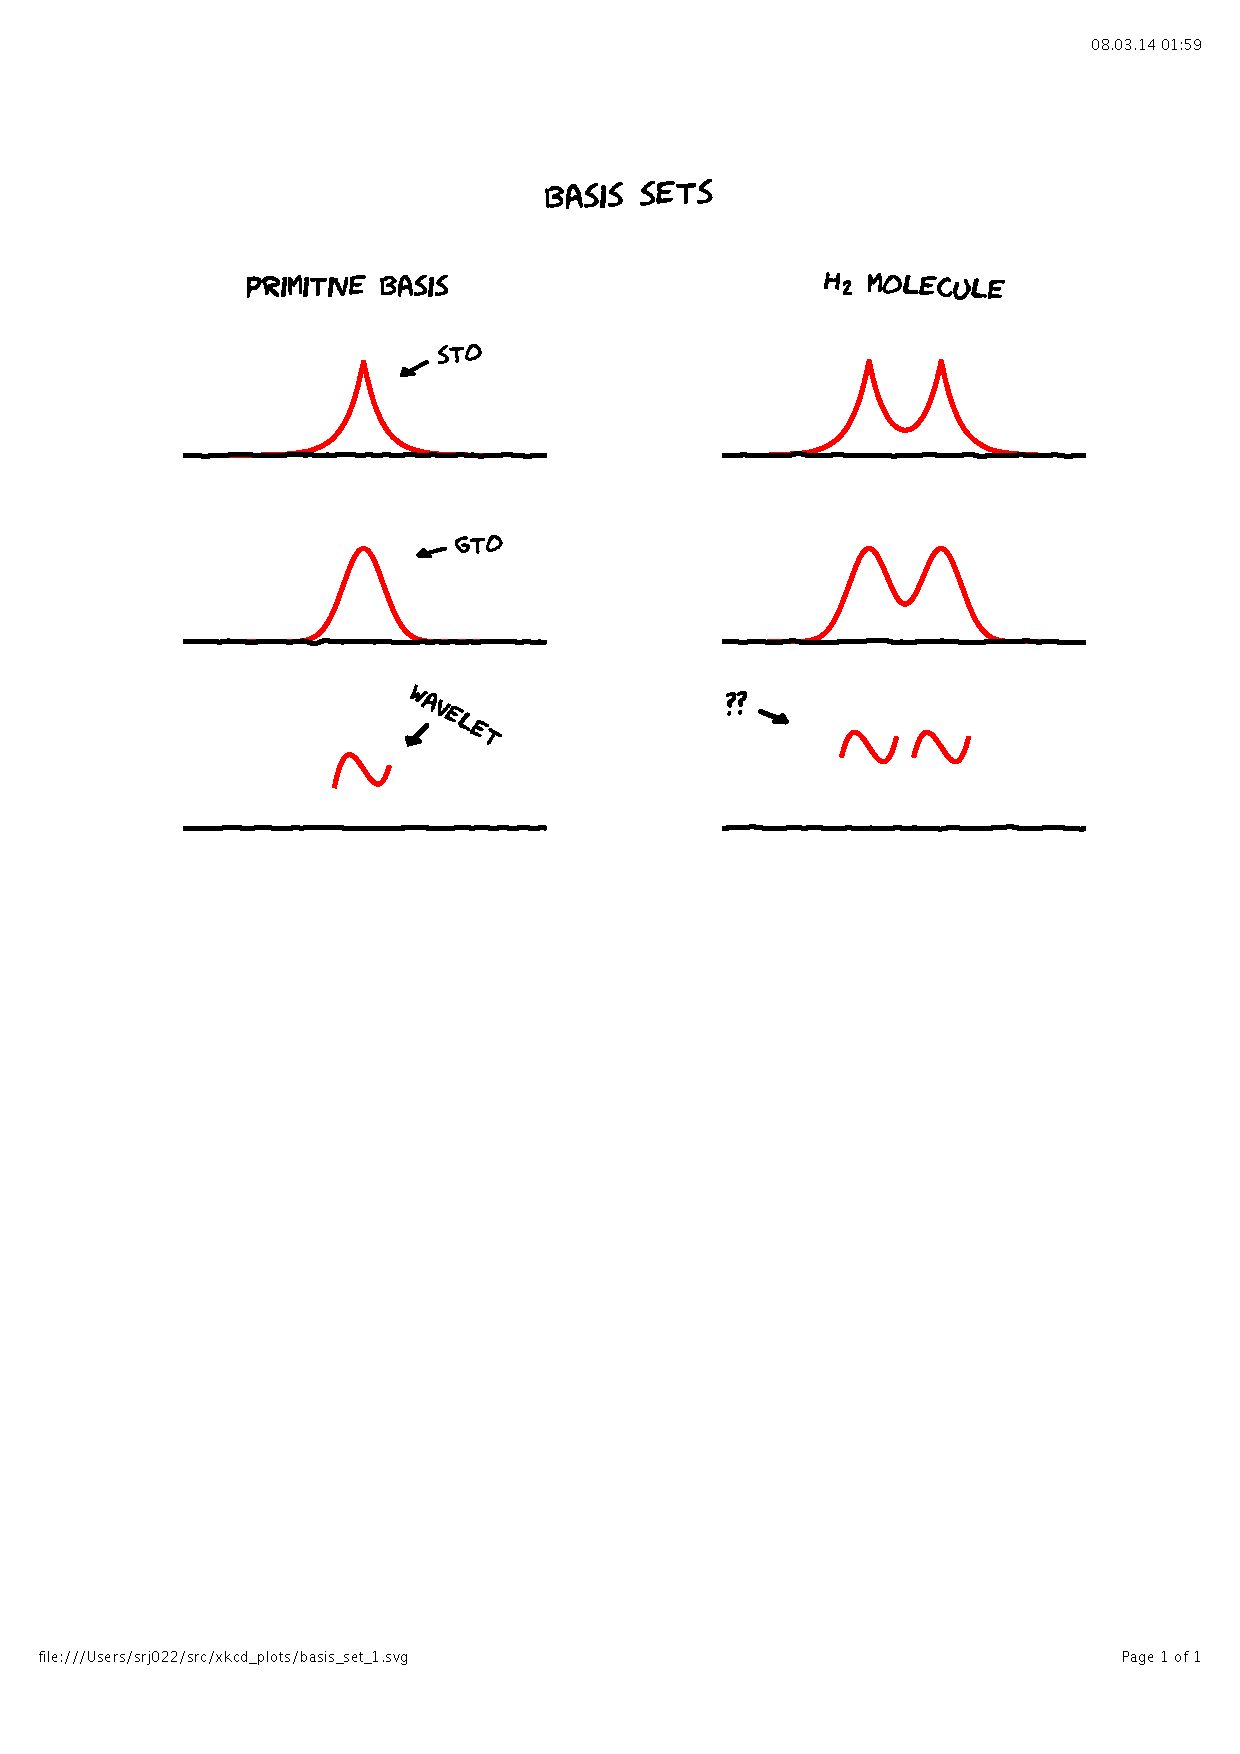
\includegraphics[scale=0.5, clip, viewport = 0 300 550 800]{figures/basis_set_1.pdf}}
    \only<2>{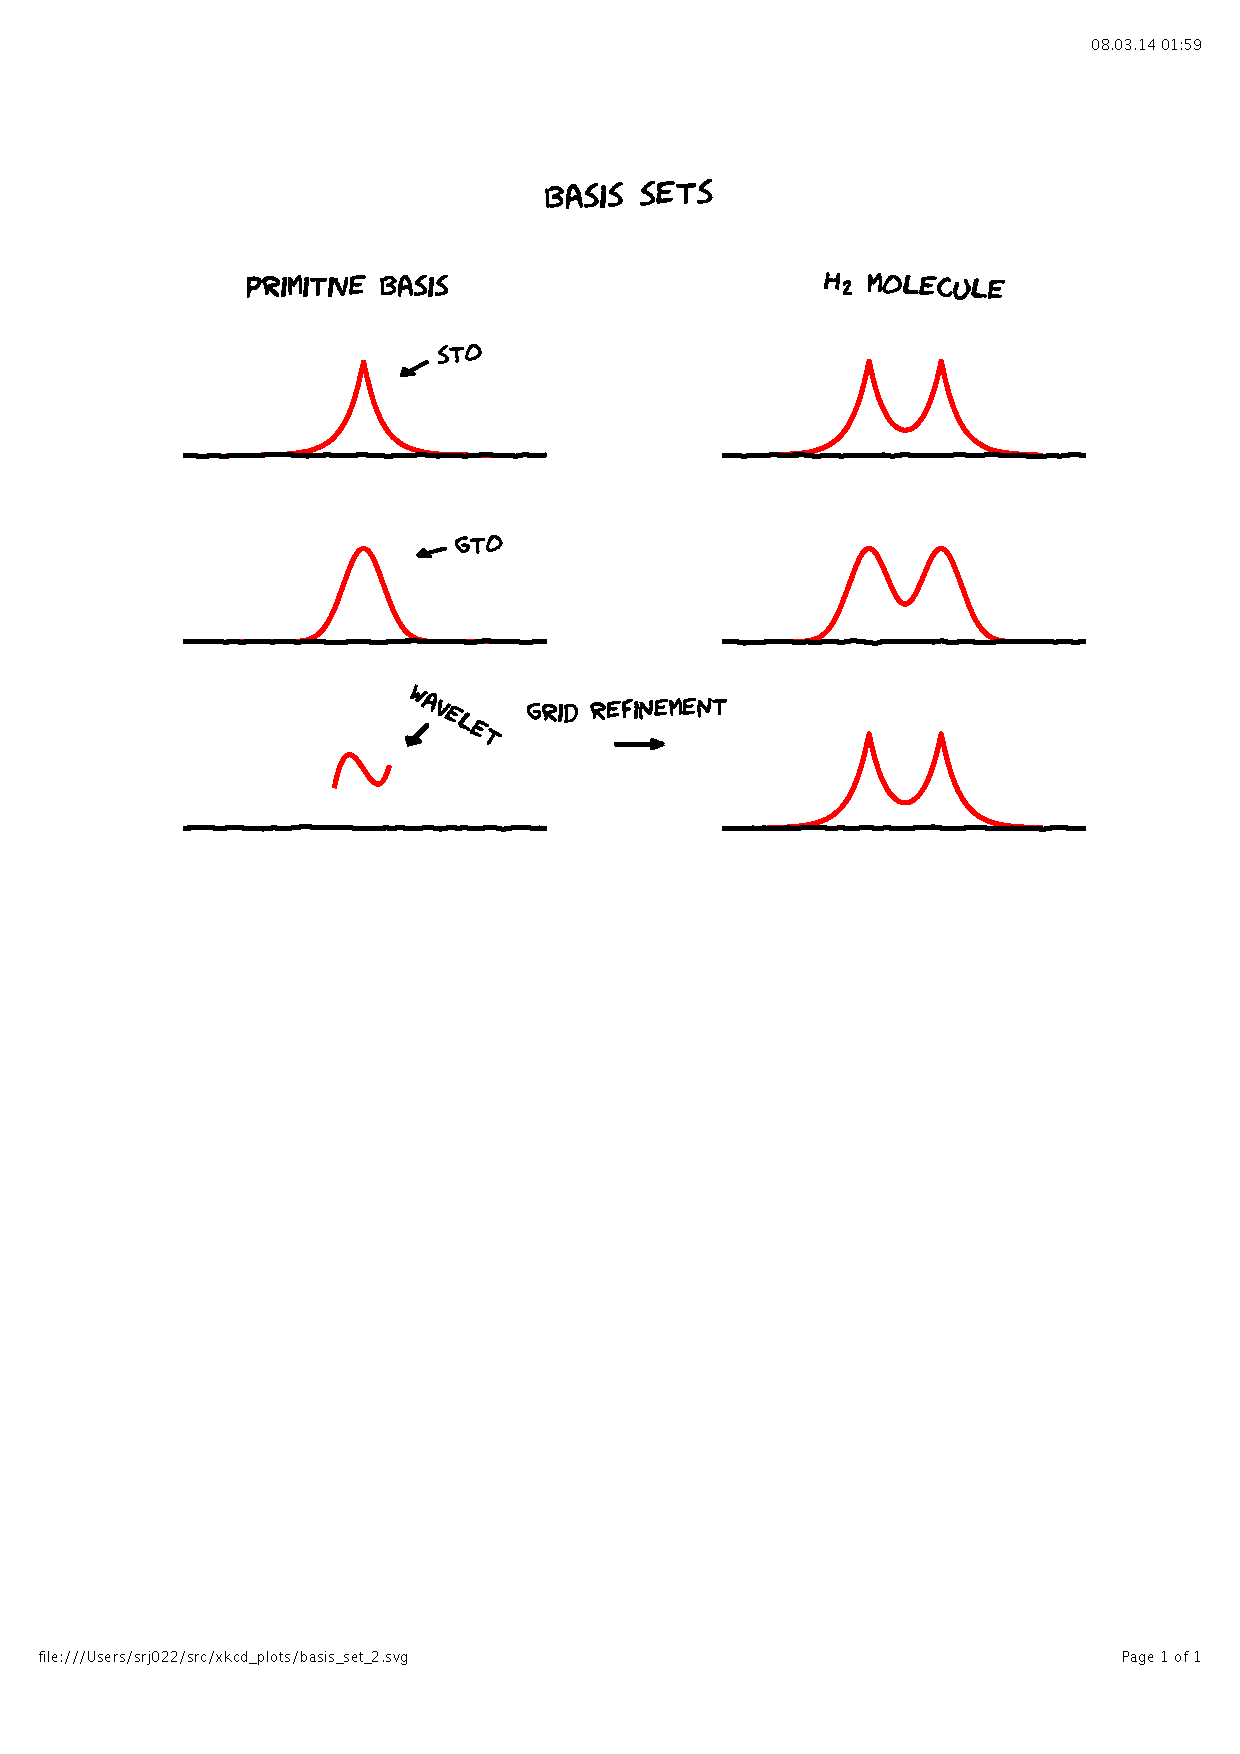
\includegraphics[scale=0.5, clip, viewport = 0 300 550 800]{figures/basis_set_2.pdf}}
    \only<3>{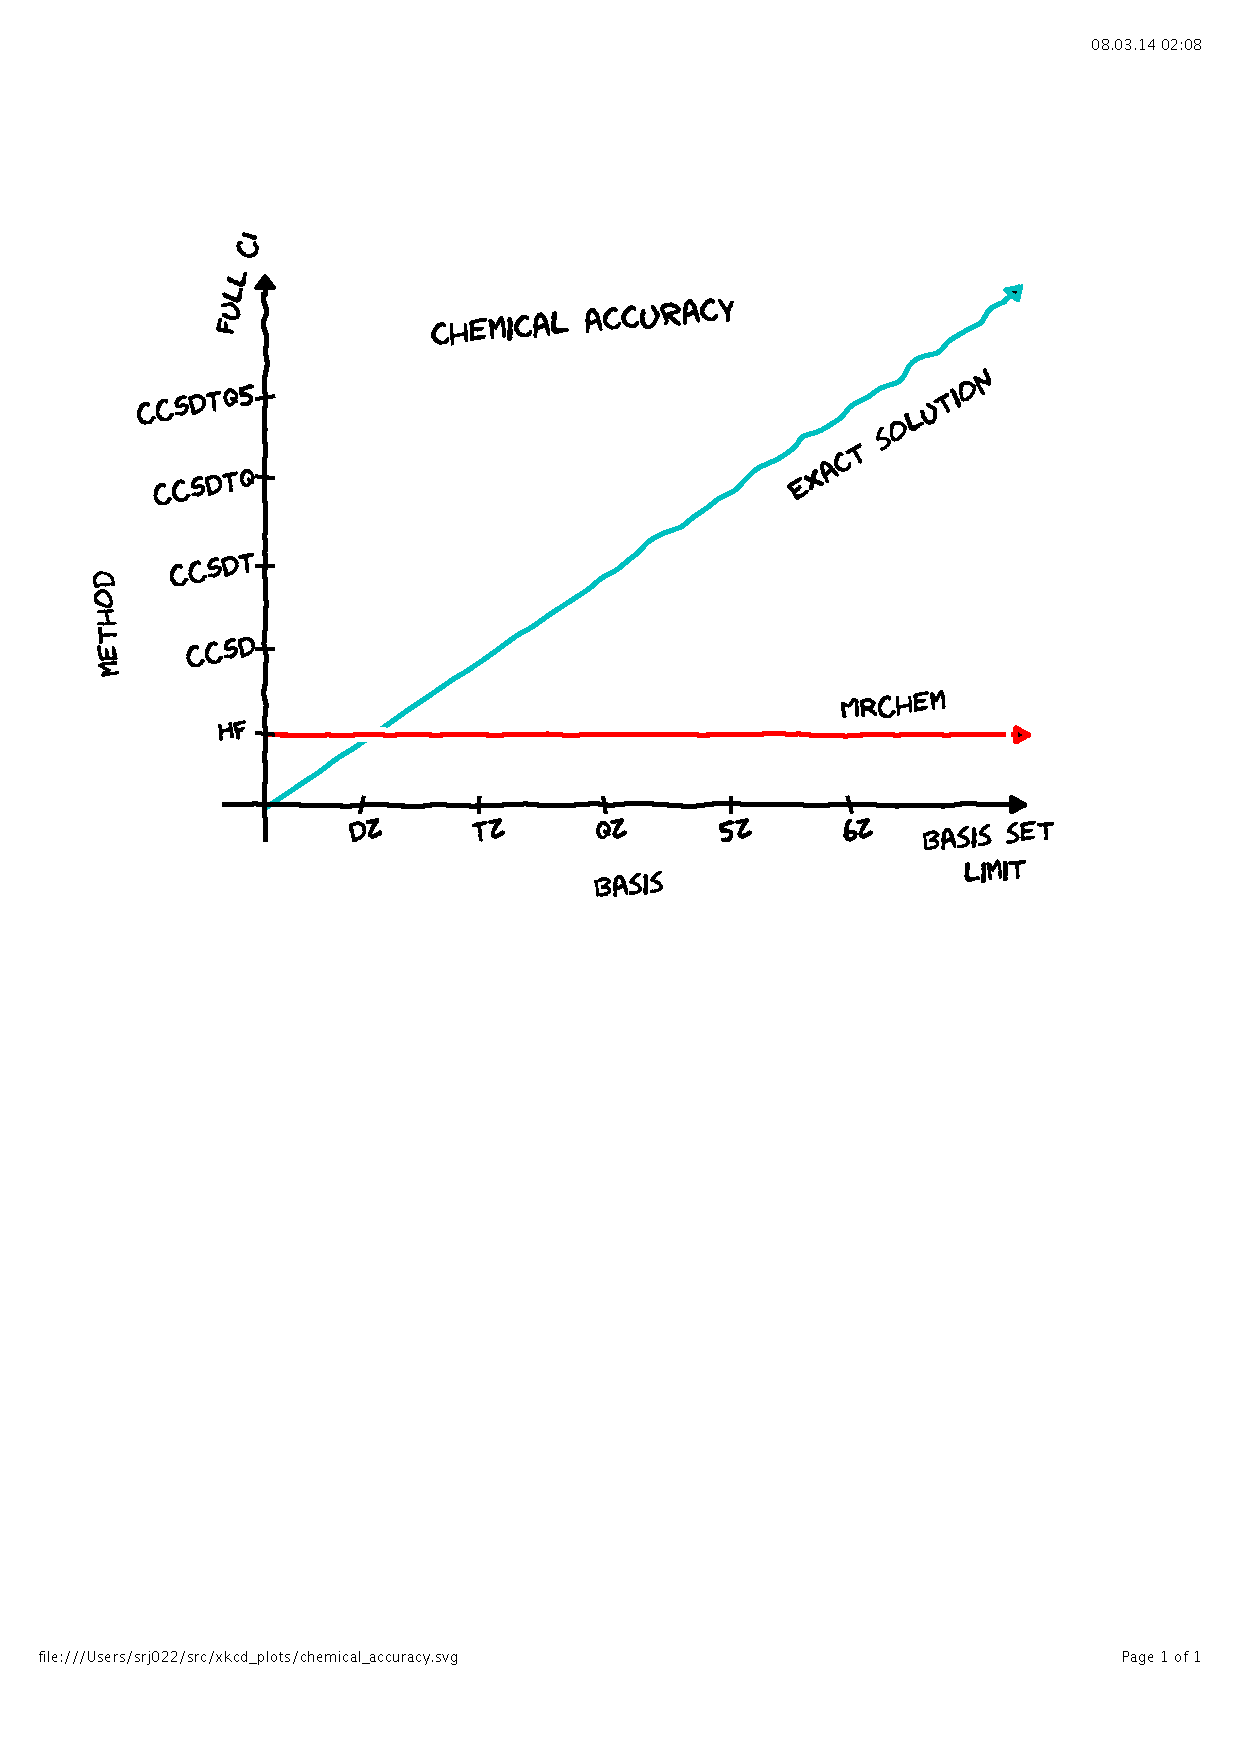
\includegraphics[scale=0.5, clip, viewport = 0 300 550 800]{figures/chemical_accuracy.pdf}}
    \end{center}
\end{frame}

\begin{frame}
    \frametitle{Integral formulation}
    The Kohn-Sham equations are rewritten
    \begin{align}
	\nonumber
	\left[-\frac{1}{2}\nabla^2 + v_{eff}(\boldsymbol{r})\right]
	\phi_i(\boldsymbol{r}) =&\ \epsilon_i \phi(\boldsymbol{r})\\
	\nonumber
	\ & \ \\
	\nonumber
	\left[-\nabla^2 - 2\epsilon_i\right]\phi_i(\boldsymbol{r}) =&\ 
	    -2\ v_{eff}(\boldsymbol{r})\phi_i(\boldsymbol{r})\\
	\nonumber
	\phi_i(\boldsymbol{r}) =&\ -2\int H^{\mu}(\boldsymbol{r}-\boldsymbol{r}')\
	    \left[v_{eff}(\boldsymbol{r}') \phi_i(\boldsymbol{r}')\right] d\boldsymbol{r}'
    \end{align}
    \ \\
    \ \\
    using the BSH Green's kernel with $\mu = \sqrt{-2\epsilon_i}$.\\
    \ \\
    \ \\
    Solved self-consistently by iterative techniques\\
    \begin{equation}
	\nonumber
	\phi_i^{n+1} =\ -2\hat{H}^n\left[v_{eff}^n\phi_i^n\right]
    \end{equation}
    \ \\
    \ \\
    \tiny \it{M. H. Kalos; "Monte Carlo calculations of the ground state of three- and 
	    four-body nuclei", Physical Review (1962)}
\end{frame}

\begin{frame}
    \frametitle{Hydrogen atom}
    \begin{columns}
    \begin{column}{.50\textwidth}
    \centering
    The equation is solved iteratively
    \begin{align}
	\nonumber
	\phi^{n+1} &= -2\hat{H}^n\left[v_{nuc}\phi^n\right]\\
	\nonumber
	\Delta\phi^n &= \phi^{n+1} - \phi^n
    \end{align}
    \end{column}
    \begin{column}{.50\textwidth}
    \centering
    The energy update is calculated from the orbital update
    \begin{equation}
	\nonumber
	\Delta \epsilon^n = \left<\phi^{n+1}|v_{nuc}|\Delta\phi^n\right>
    \end{equation}
    \end{column}
    \end{columns}    
    \begin{center}
	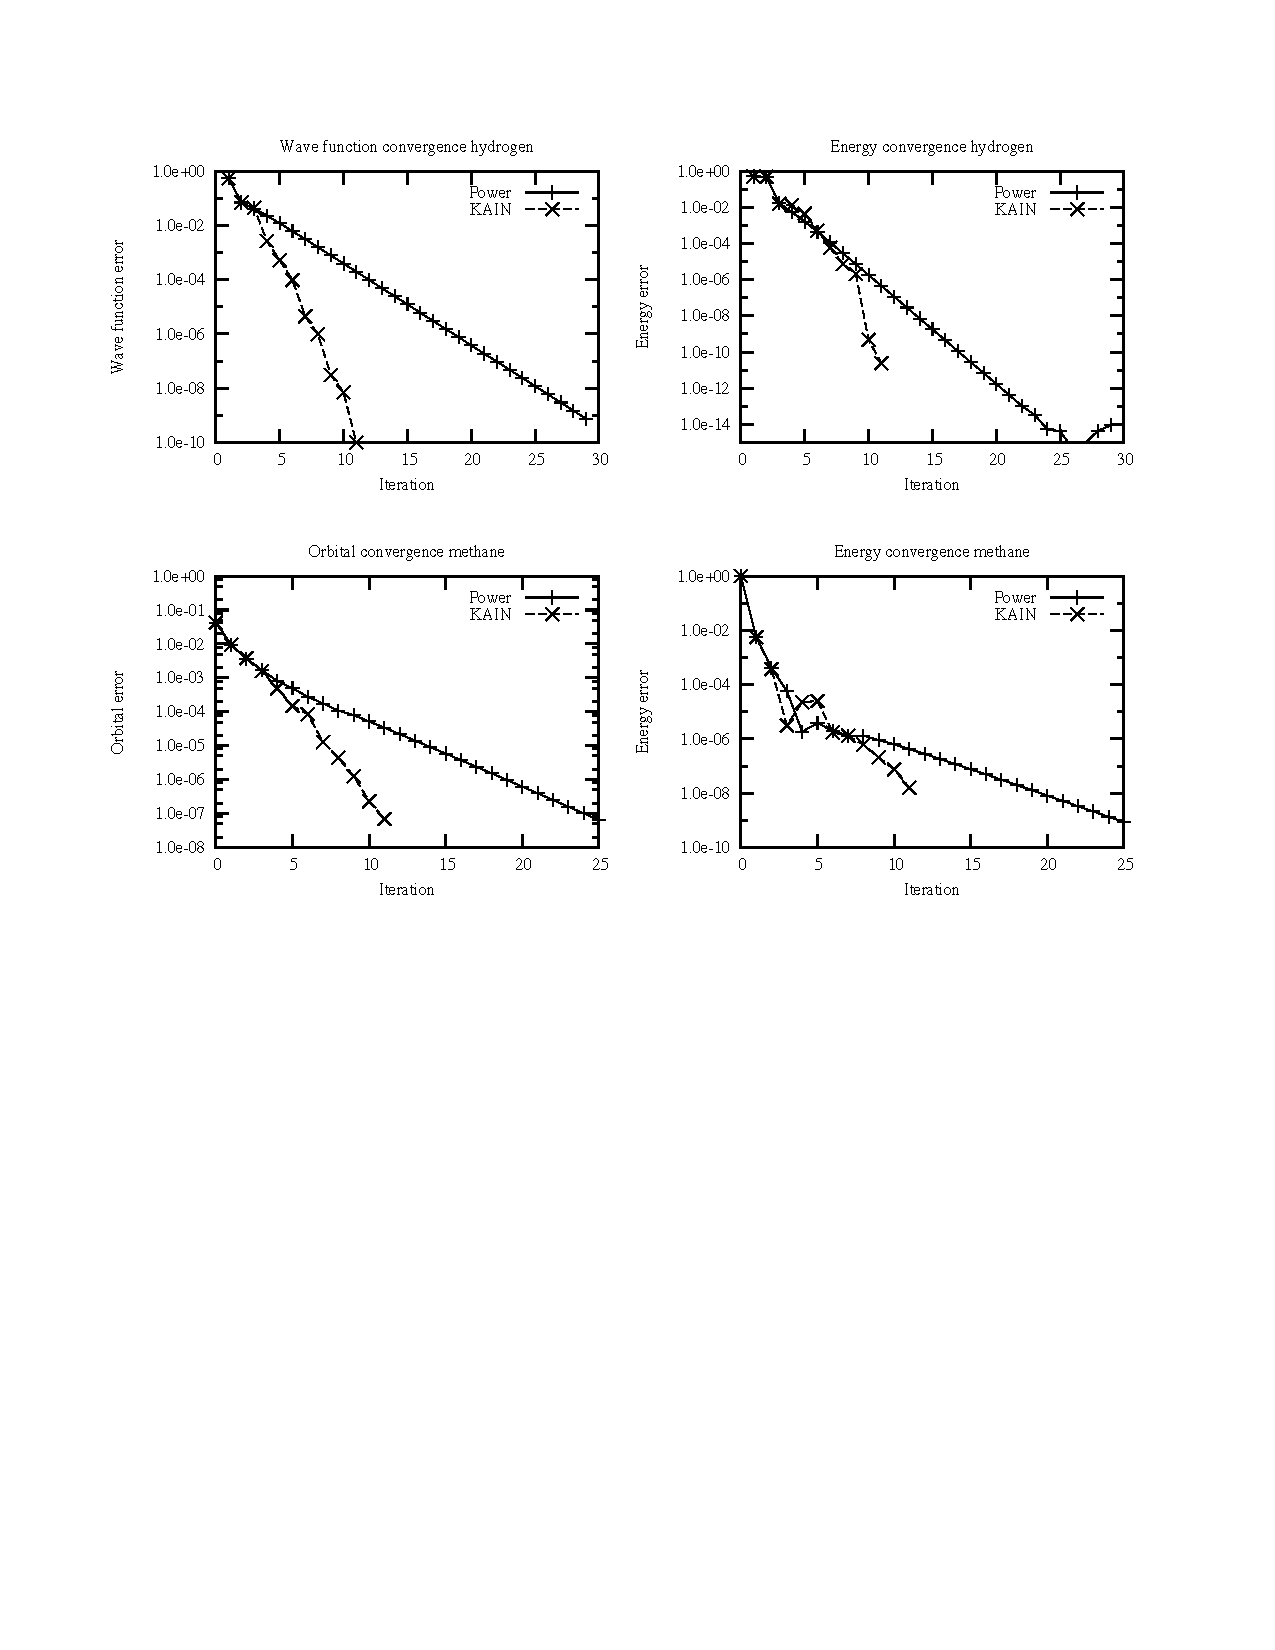
\includegraphics[scale=0.6, clip, viewport = 50 550 540 730]{figures/convergence.pdf}
    \end{center}
\end{frame}

\begin{frame}
    \frametitle{Hydrogen atom}
    \only<1>{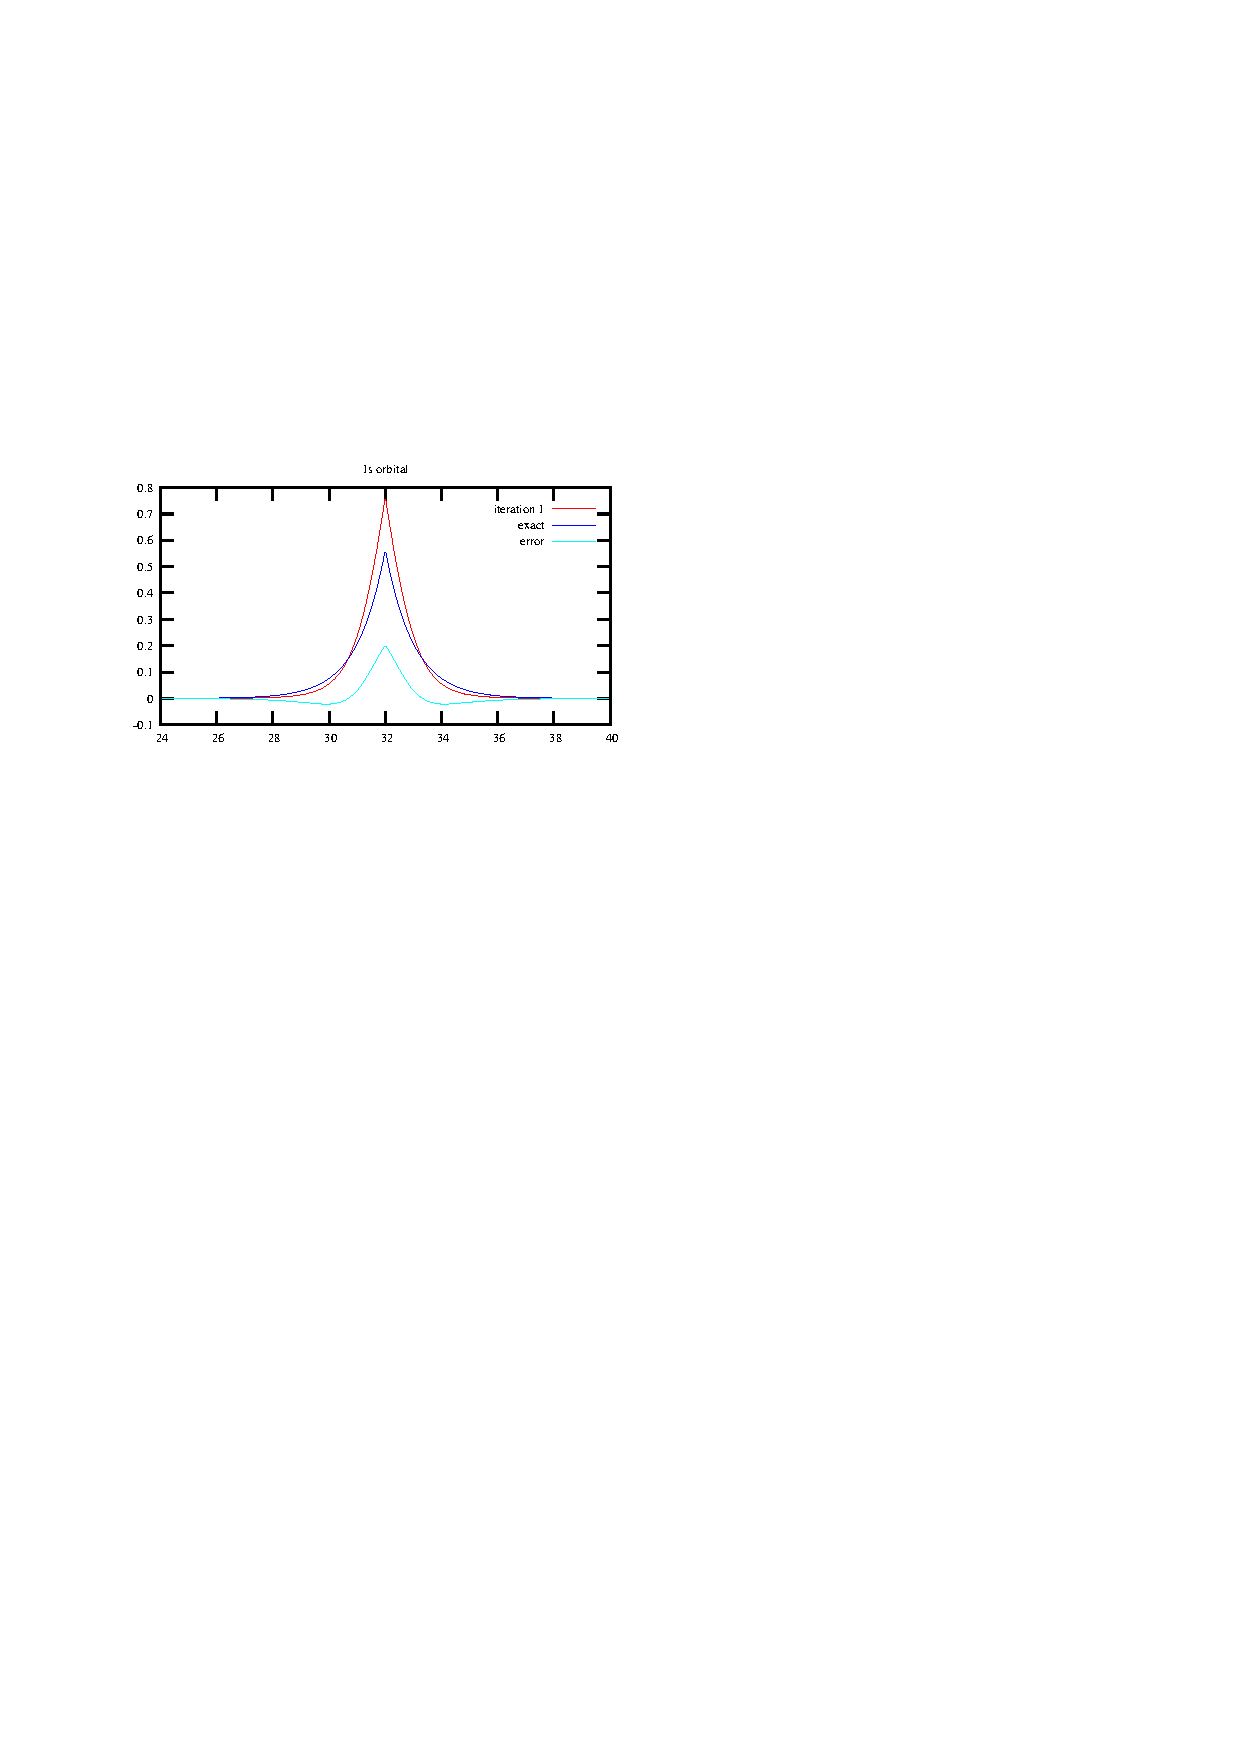
\includegraphics[viewport = 50 430 300 640, clip, scale=1.2]{figures/s1Orb_1.pdf}}
    \only<2>{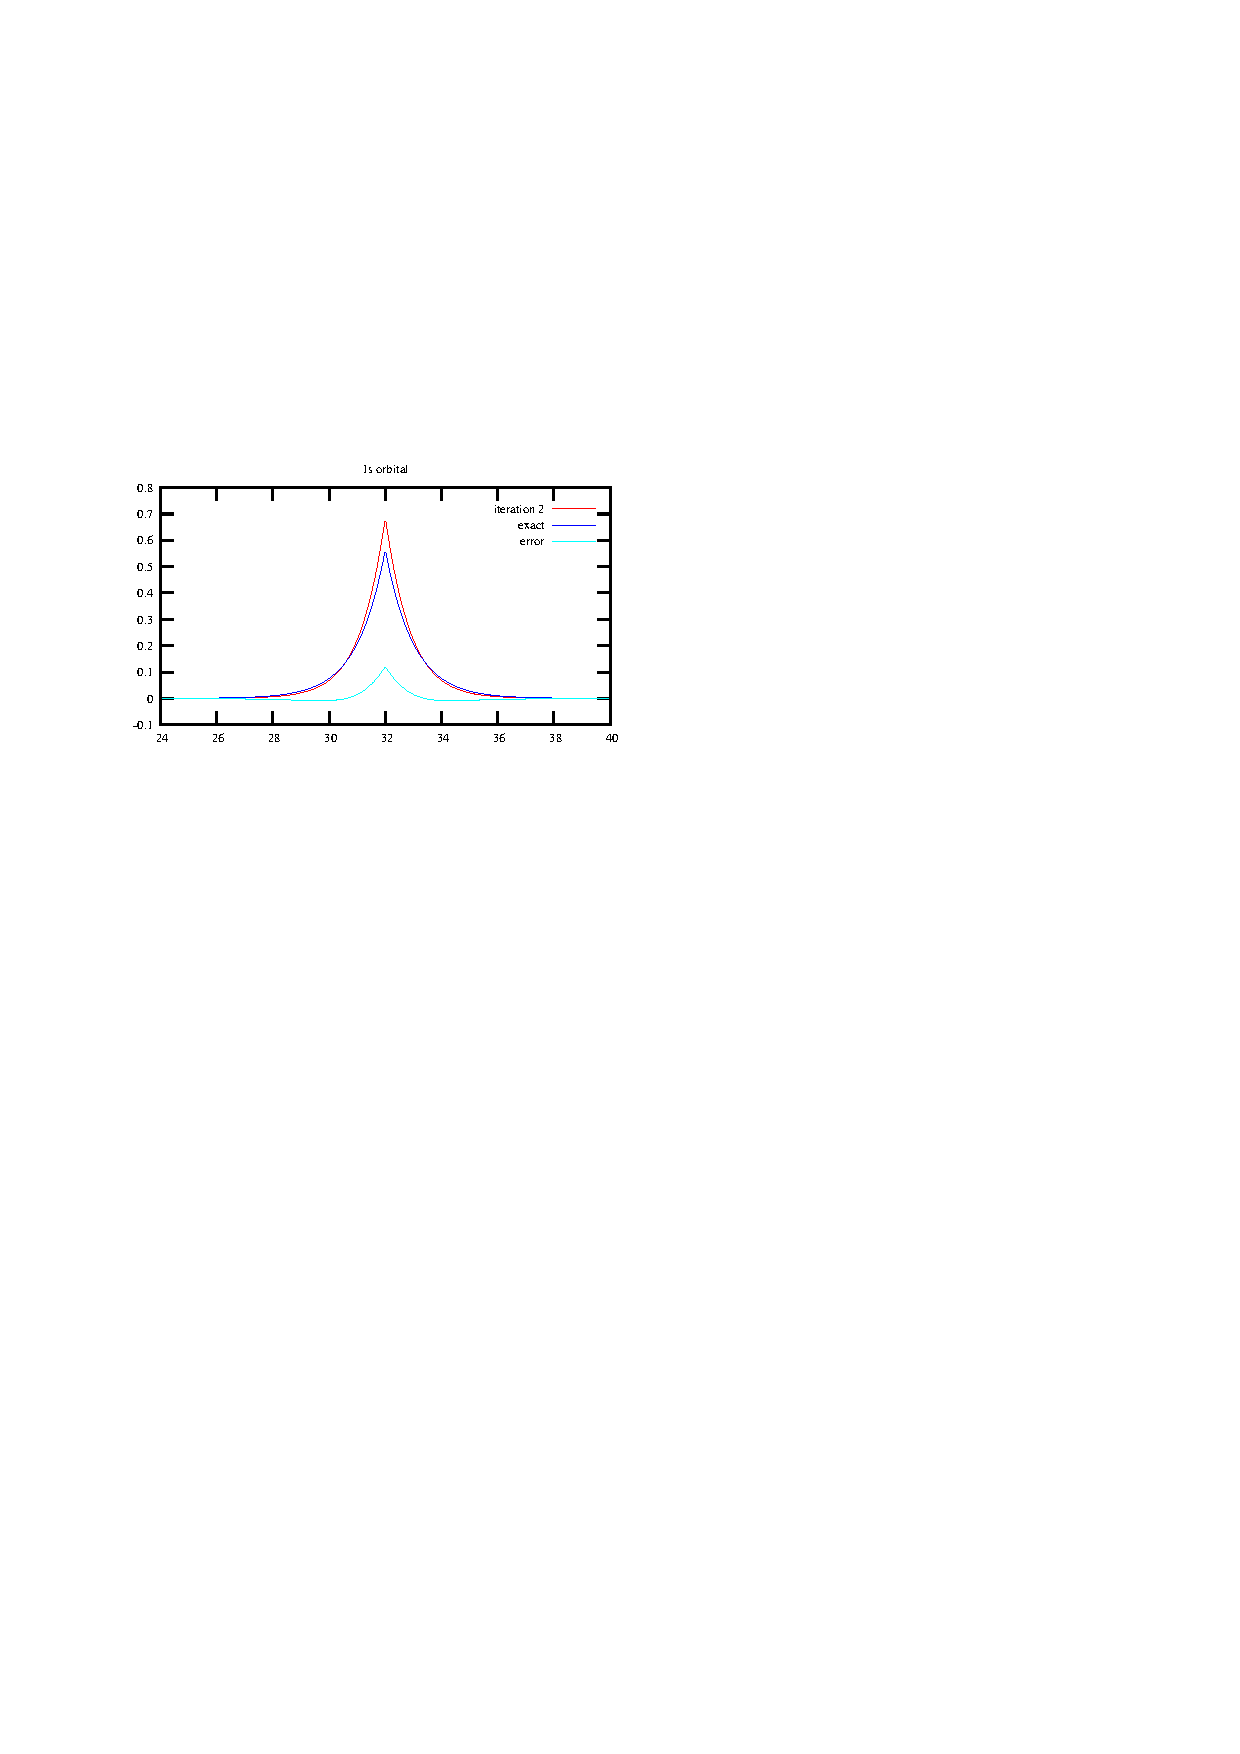
\includegraphics[viewport = 50 430 300 640, clip, scale=1.2]{figures/s1Orb_2.pdf}}
    \only<3>{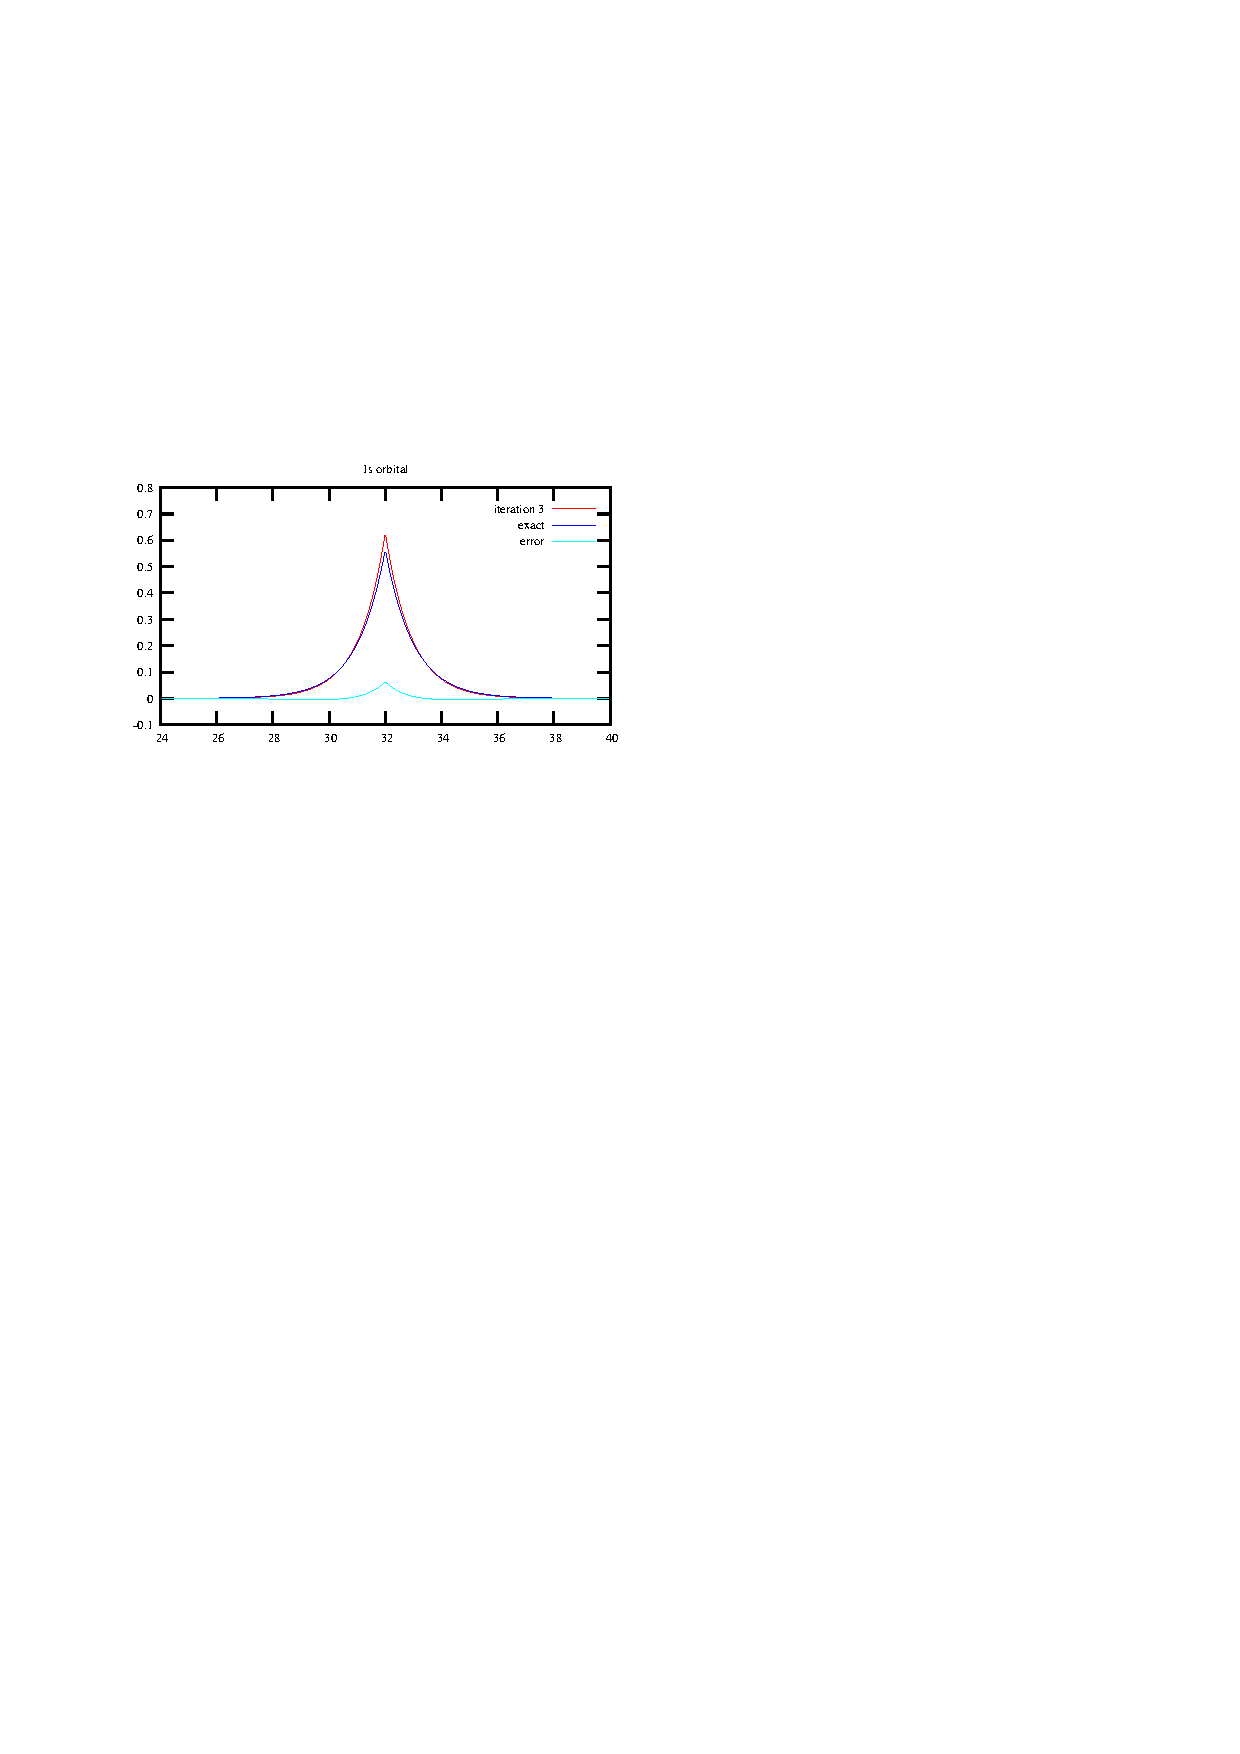
\includegraphics[viewport = 50 430 300 640, clip, scale=1.2]{figures/s1Orb_3.pdf}}
    \only<4>{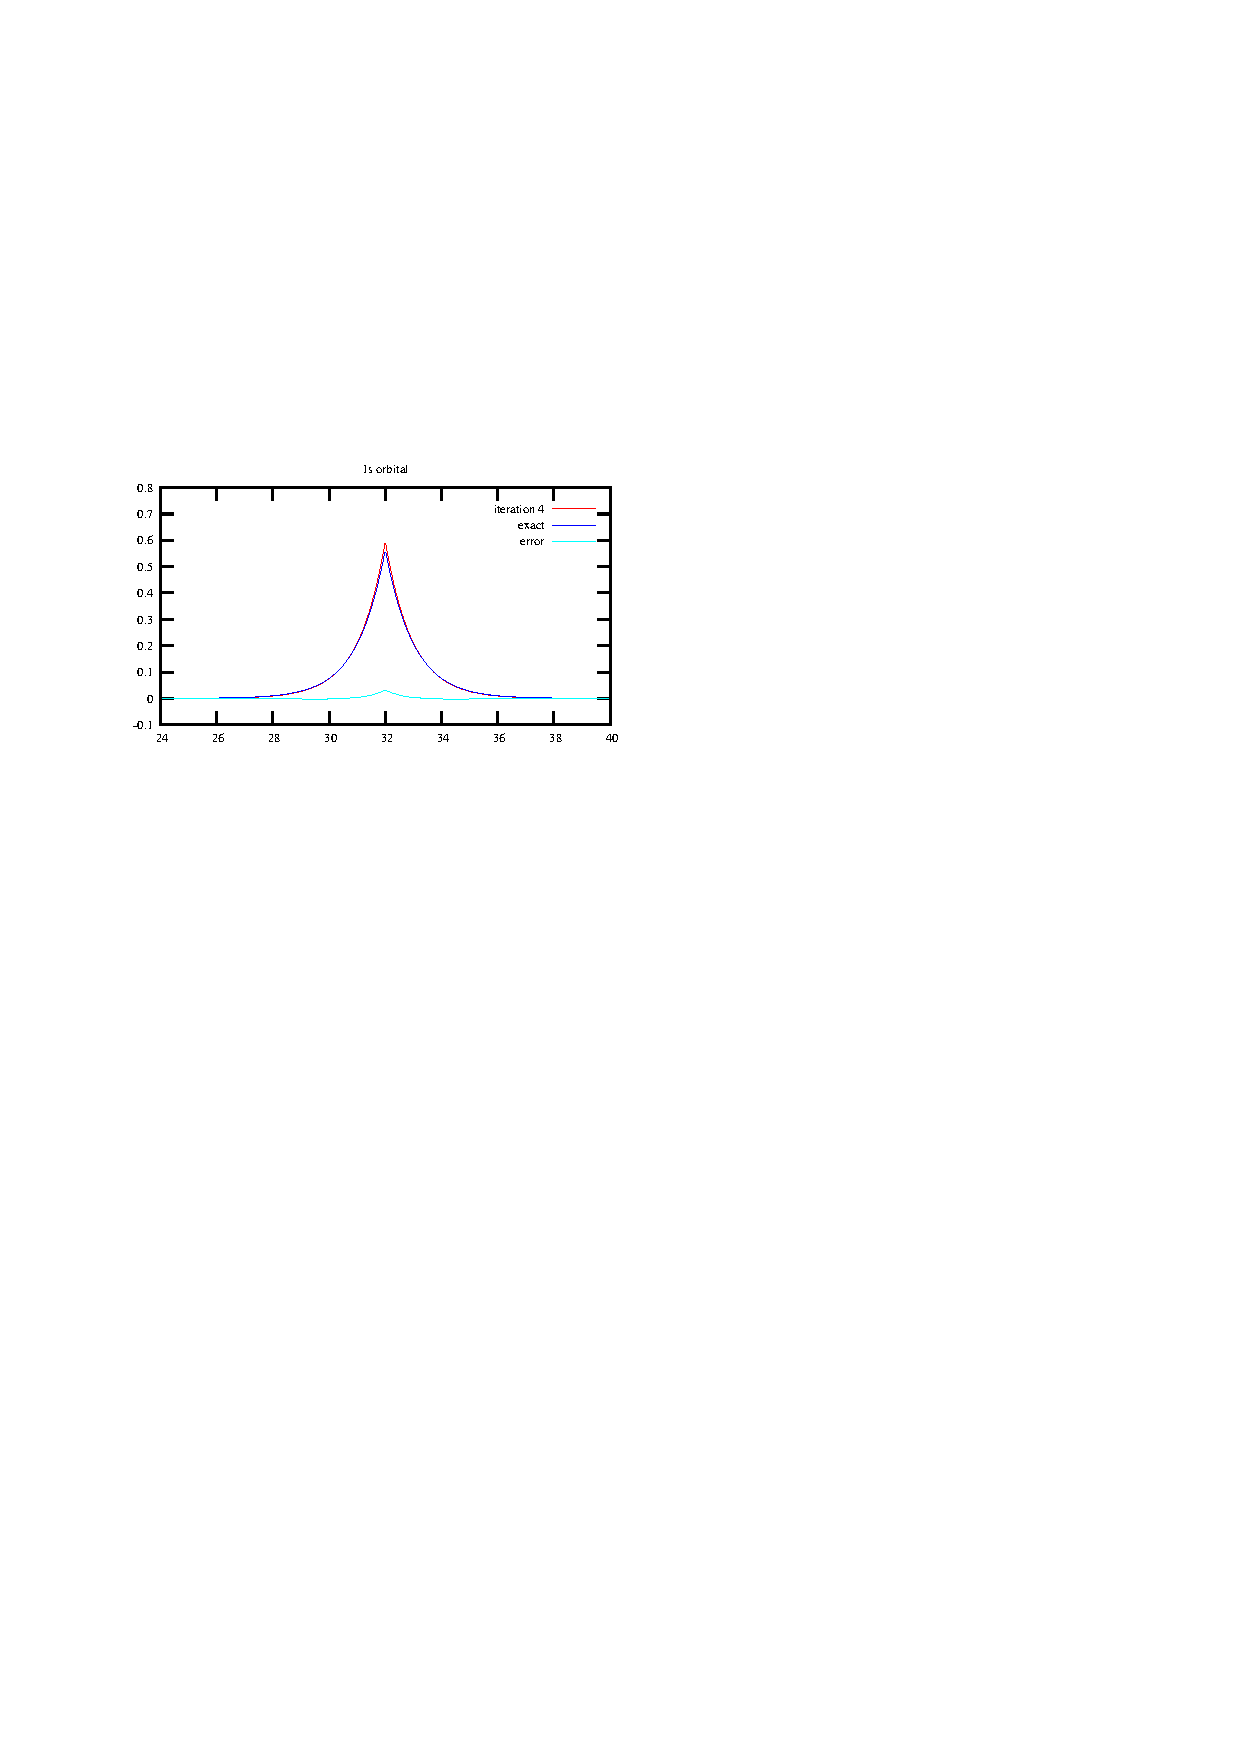
\includegraphics[viewport = 50 430 300 640, clip, scale=1.2]{figures/s1Orb_4.pdf}}
    \only<5>{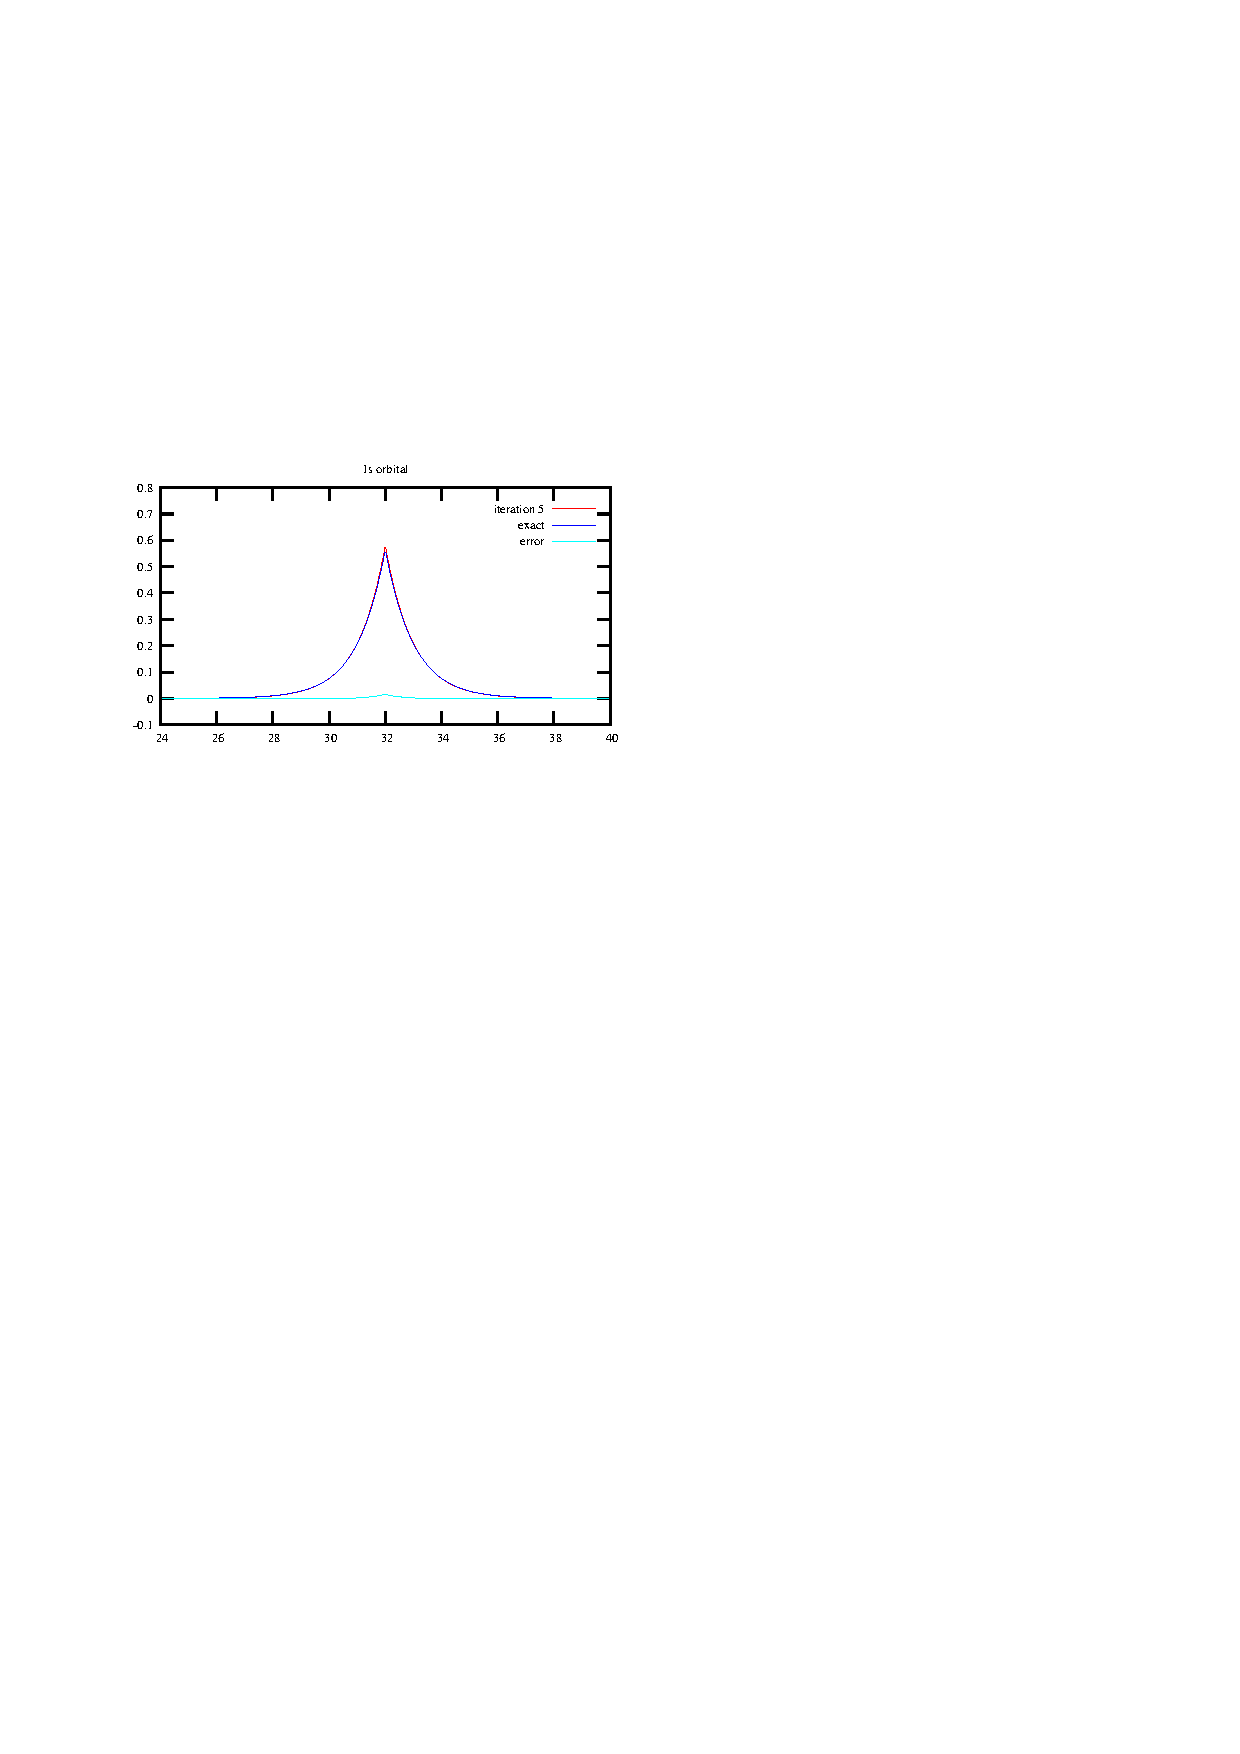
\includegraphics[viewport = 50 430 300 640, clip, scale=1.2]{figures/s1Orb_5.pdf}}
    \only<6>{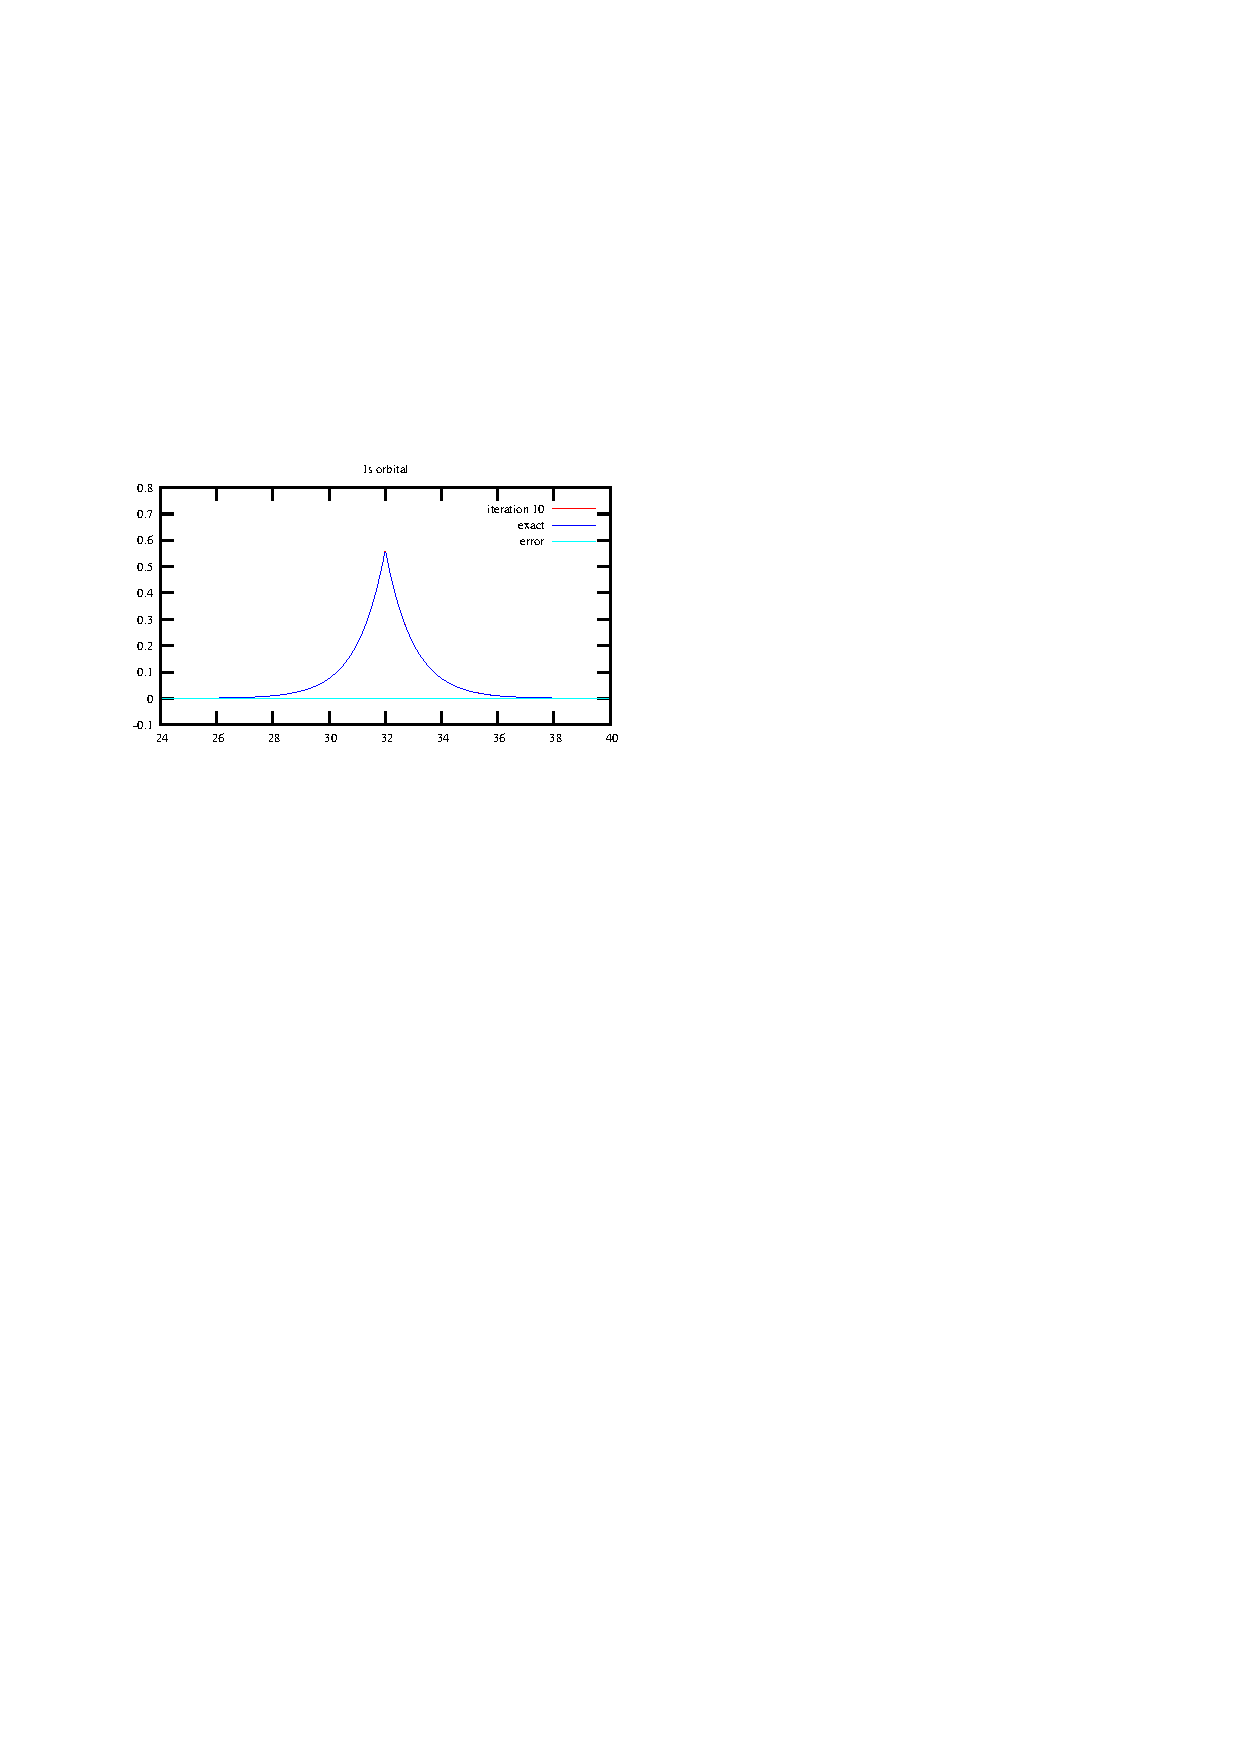
\includegraphics[viewport = 50 430 300 640, clip, scale=1.2]{figures/s1Orb_10.pdf}}
\end{frame}

\begin{frame}
    \frametitle{Many-electron systems}
    \begin{minipage}[b]{\linewidth}
    Compute density and potentials
    \begin{equation}
	\rho^n(\boldsymbol{r}) = \sum_i^N |\phi_i^n(\boldsymbol{r})|^2, \qquad \qquad 
	\rho^n(\boldsymbol{r}) \rightarrow v_{eff}^n(\boldsymbol{r})
    \end{equation}
    Iterate the Kohn-Sham equations for each orbital
    \begin{equation}
	\phi_i^{n+1} = -2\hat{H}\left[v_{eff}^n\phi_i^n\right]
    \end{equation}
    \end{minipage}
    \ \\
    \pause
    \ \\
    \begin{minipage}[b]{\linewidth}
    \only<1,2>{
    Complicating issues
    \begin{itemize}
	\item	Straightforward iteration will bring all orbitals to the
		lowest energy eigenfunction
	\item	Orthonormality must be imposed
	\item	Achieved by diagonalizing the Kohn-Sham matrix 
	\begin{equation}
	    \nonumber
	    F_{ij} = \left<\phi_i|\hat{T} + v_{eff}|\phi_j\right>
	\end{equation}
    \end{itemize}
    }
    \only<3>{
    Compute Kohn-Sham matrix update
    \begin{equation}
	\Delta F_{ij}^{n+1} = \left<\phi_i^{n+1}|v_{eff}^n |\Delta\phi_j^n\right>
			    + \left<\phi_i^{n+1}|\Delta v_{eff}^n|\phi_j^n\right>
    \end{equation}
    Diagonalize Kohn-Sham matrix\\
    \ \\
    Compute iterative subspace updates (KAIN)\\
    \ \\
    Orthonormalize
    }
    \end{minipage}
\end{frame}

\begin{frame}
    \frametitle{Many-electron systems}
    \begin{columns}
    \begin{column}[b]{0.20\linewidth}
	\ \\
	\ \\
    \end{column}
    \begin{column}[b]{0.30\linewidth}
    \begin{figure}
	\centering
	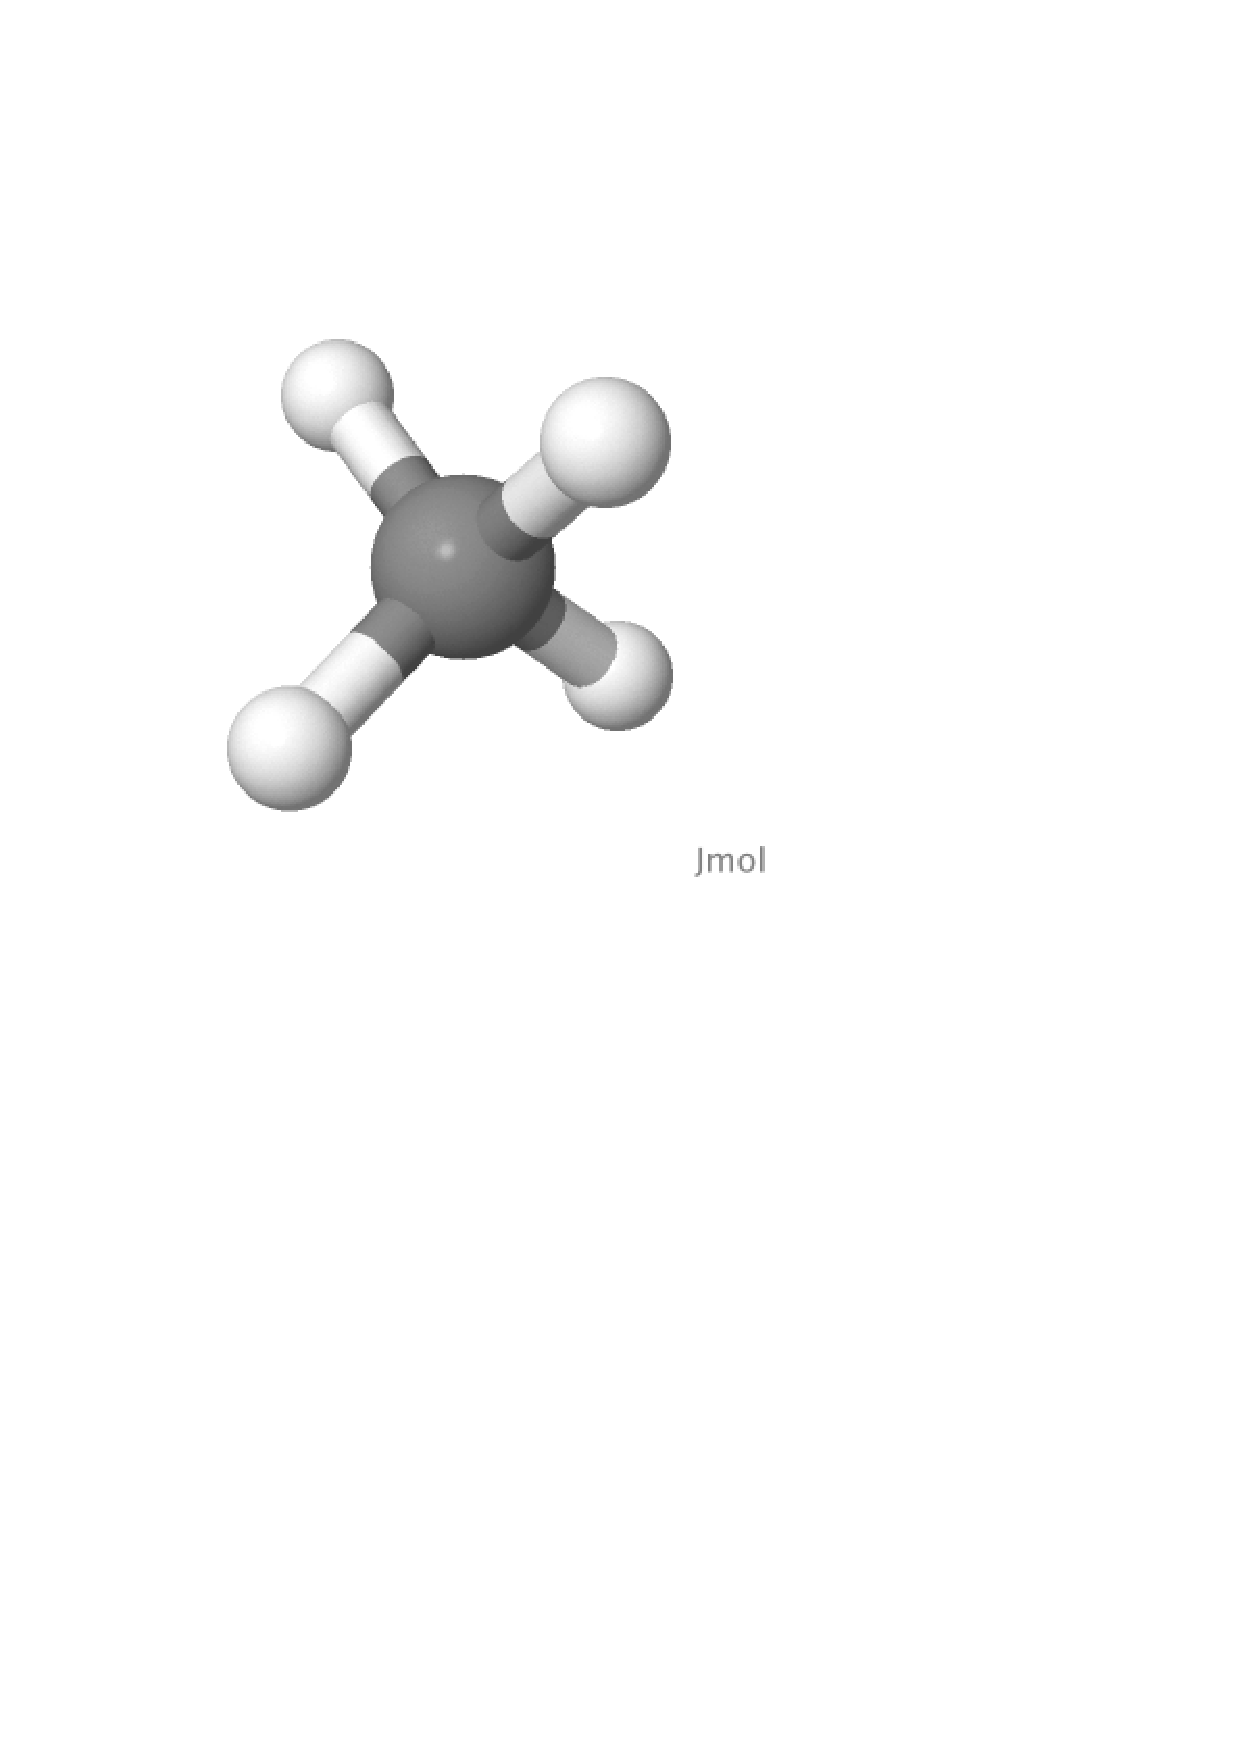
\includegraphics[scale=0.2, clip, viewport = 60 450 600 720]{figures/methane.pdf}\\
	\ \\
	\ \\
    \end{figure}
    \end{column}
    \begin{column}[b]{0.50\linewidth}
    \begin{figure}
	\begin{center}
	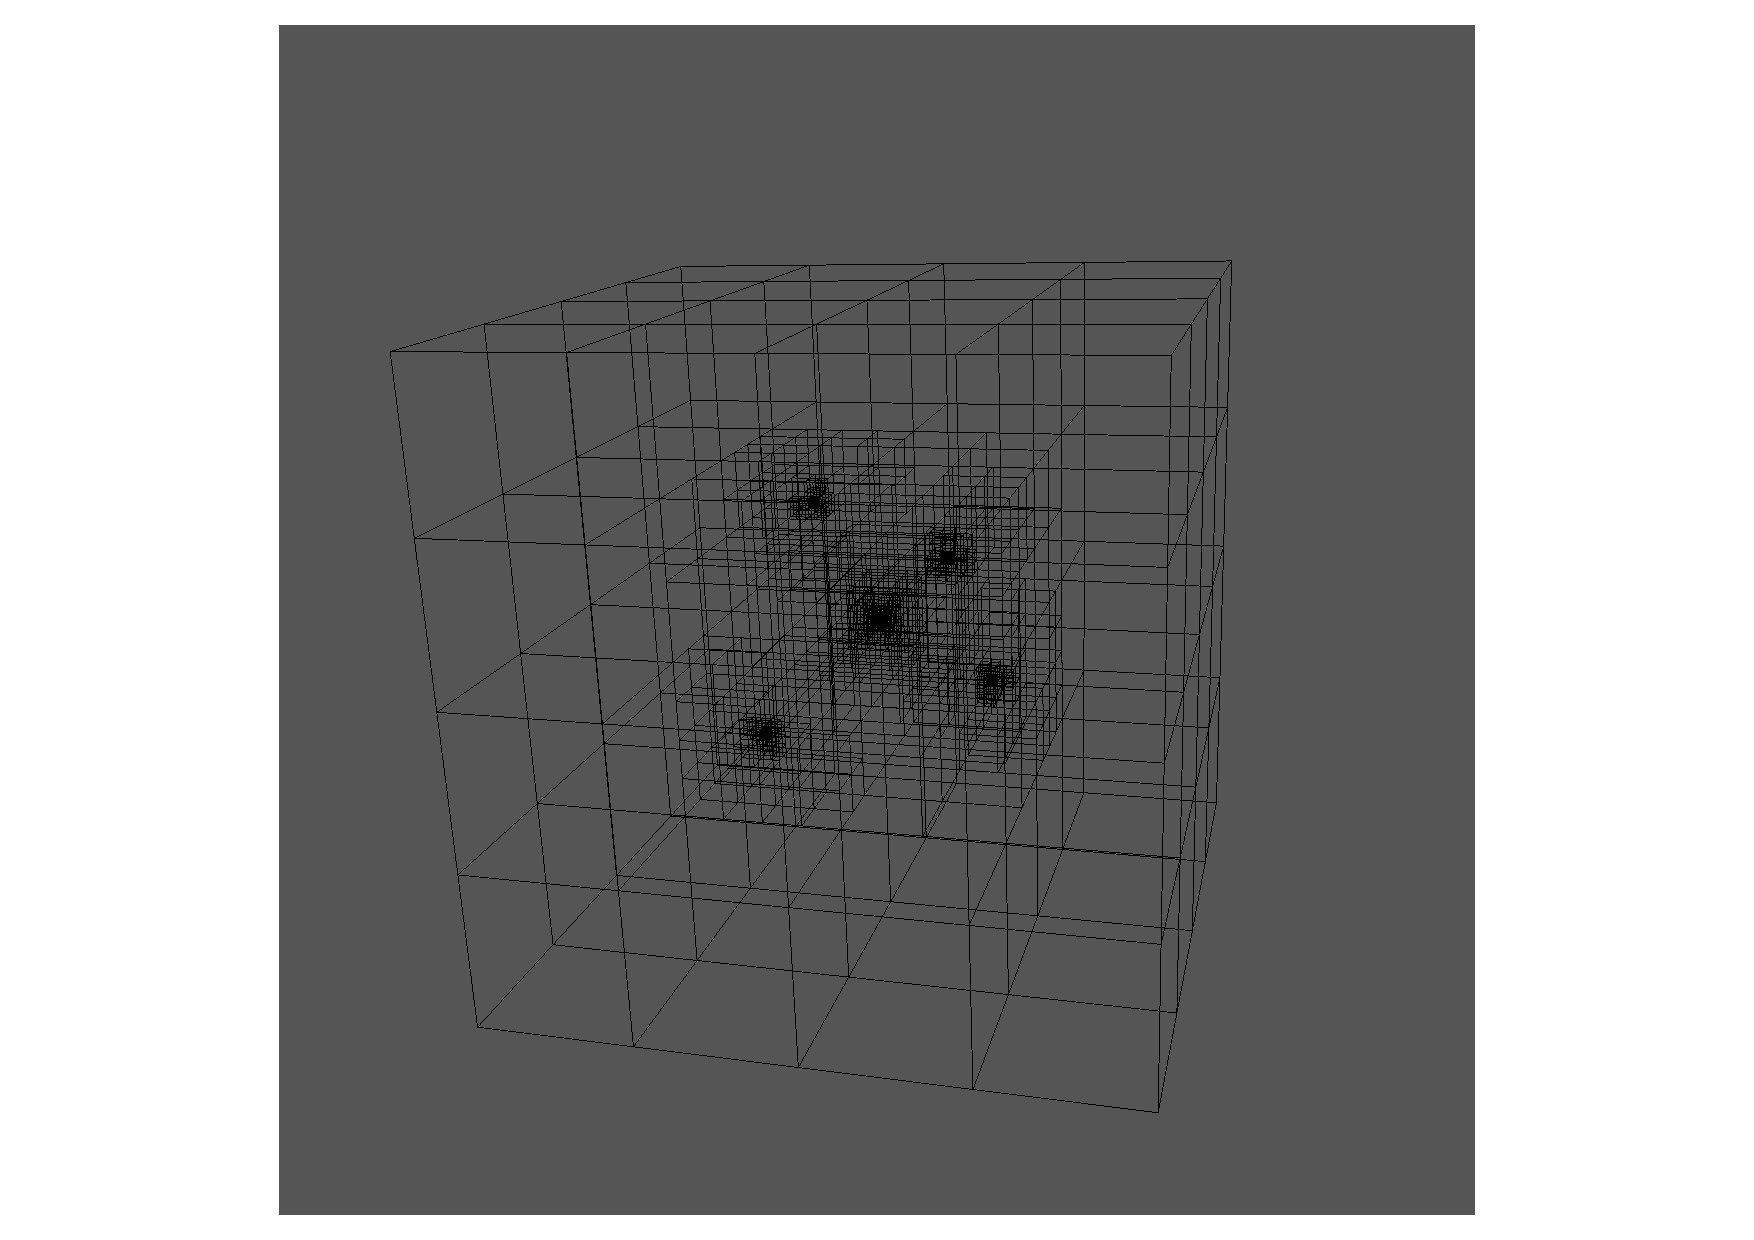
\includegraphics[scale=0.45, clip, viewport = 320 200 520 400]{figures/methaneGrid.pdf}\\
	\end{center}
    \end{figure}
    \end{column}
    \end{columns}
    \begin{center}
	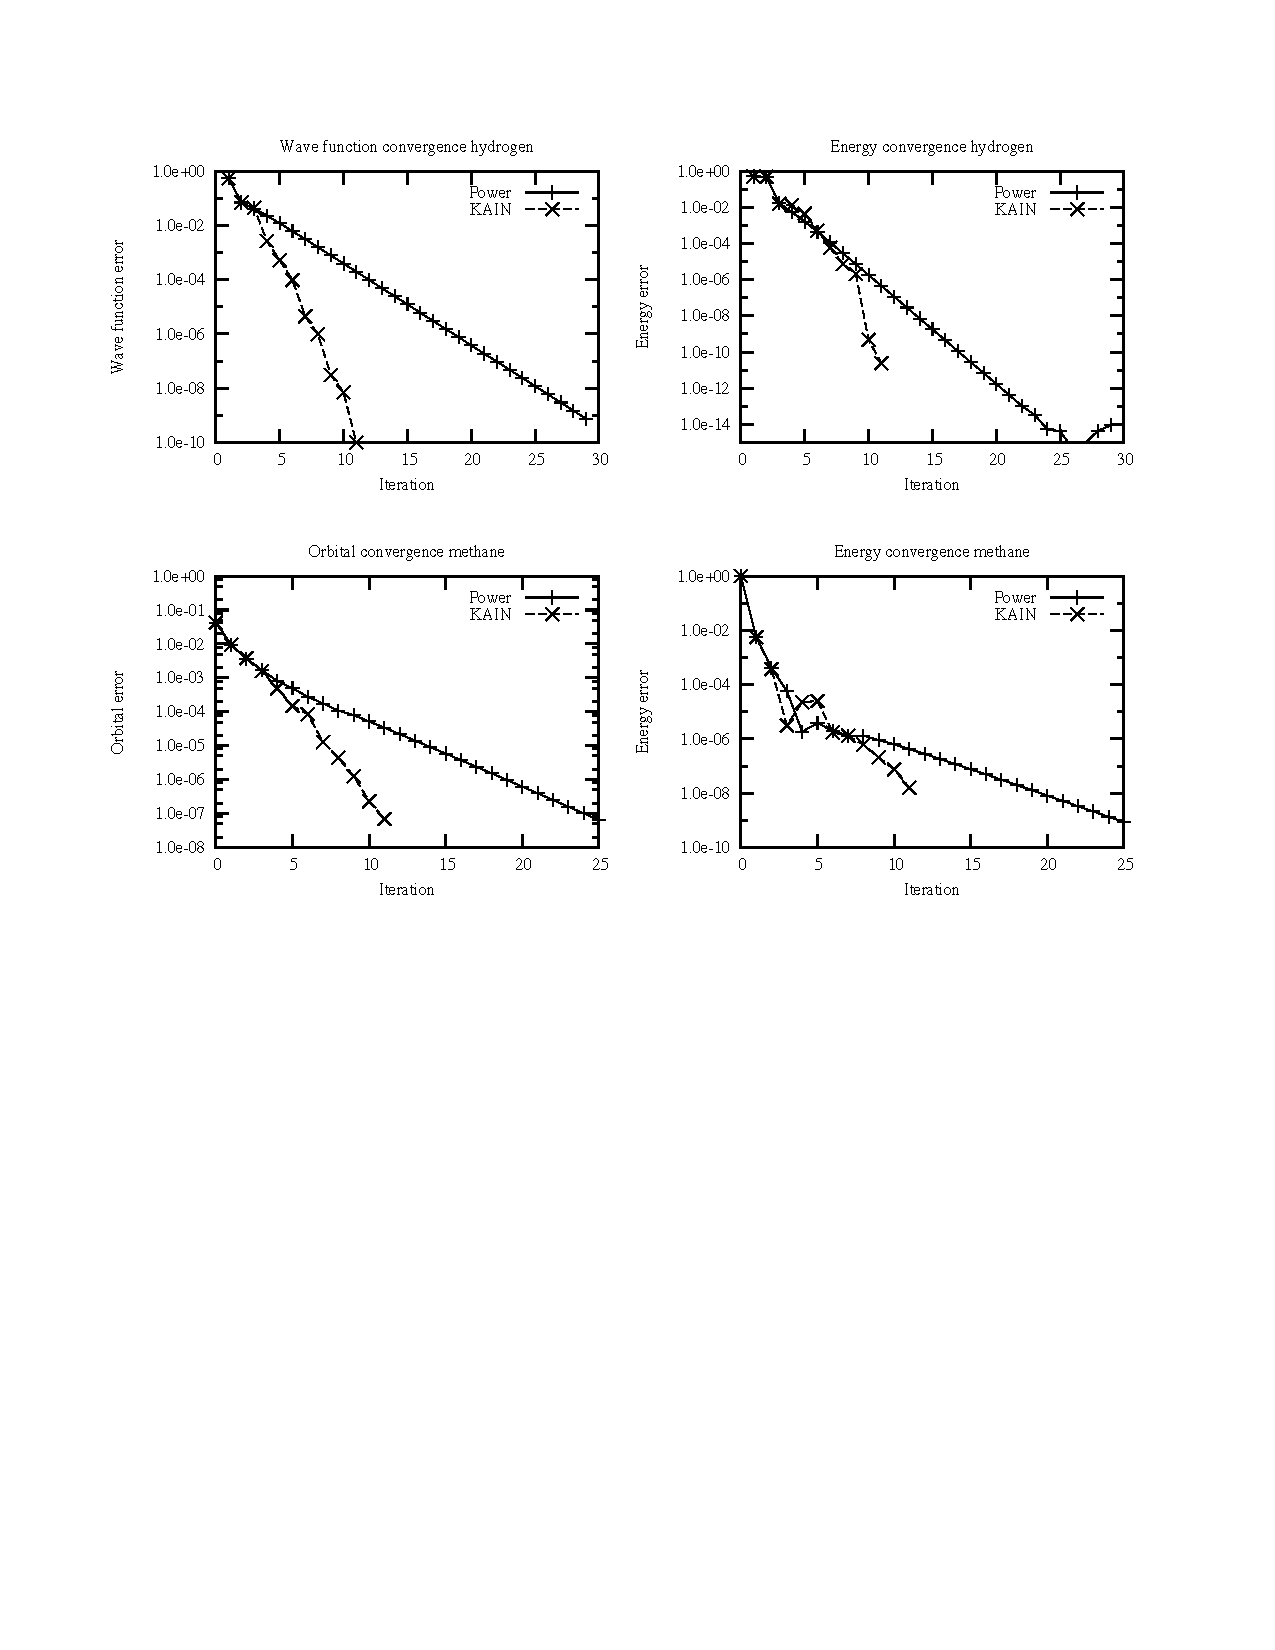
\includegraphics[scale=0.6, clip, viewport = 50 350 550 540]{figures/convergence.pdf}
    \end{center}
\end{frame}

\begin{frame}
    \frametitle{Many-electron systems}
    \begin{center}
	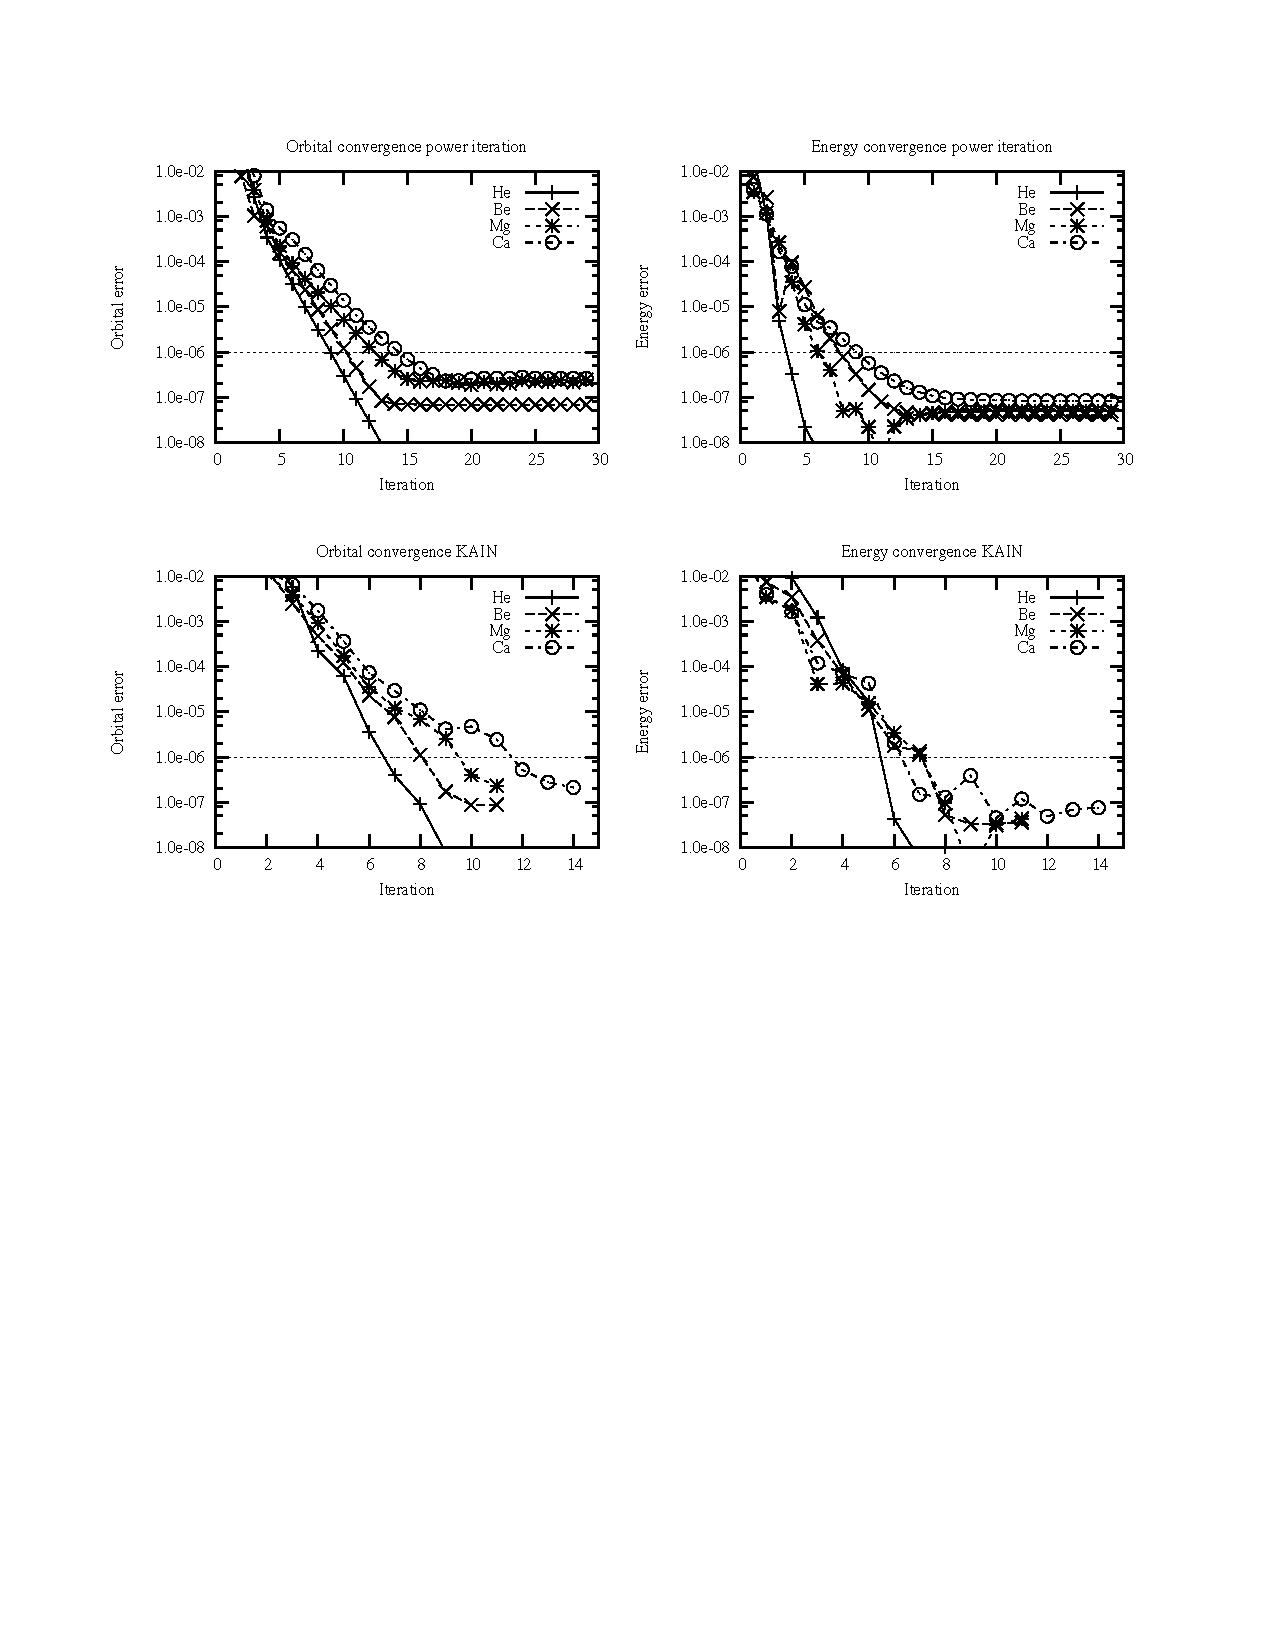
\includegraphics[scale=0.6, clip, viewport = 50 550 550 740]{figures/accuracy.pdf}
    \end{center}
\end{frame}

\begin{frame}
    \frametitle{Orbital localization}
    Total energy invariant under unitary transformations among occupied orbitals
    \begin{equation}
	\varphi_i(\boldsymbol{r}) = \sum_j U_{ji}^\ast \phi_i(\boldsymbol{r}), \qquad \qquad U^\ast U = UU^\ast = I
    \end{equation}
    Foster-Boys algorithm finds a matrix $U$ that leads to localized orbitals\\
    \begin{columns}
    \begin{column}[b]{0.48\linewidth}
    \begin{center}
	\only<1>{\includegraphics[scale=0.3, clip, viewport = 80 260 600 400]{figures/alkane.pdf}}
	\only<2,3>{\includegraphics[scale=0.3, clip, viewport = 80 560 600 700]{figures/alkane.pdf}}
	\only<1>{\includegraphics[scale=0.3, clip, viewport = 80 260 600 400]{figures/can_orb_1.pdf}}
	\only<2,3>{\includegraphics[scale=0.3, clip, viewport = 80 560 600 700]{figures/can_orb_1.pdf}}
	\only<1>{\includegraphics[scale=0.3, clip, viewport = 80 260 600 400]{figures/can_orb_2.pdf}}
	\only<2,3>{\includegraphics[scale=0.3, clip, viewport = 80 560 600 700]{figures/can_orb_2.pdf}}
    \end{center}
    \end{column}
    \begin{column}[b]{0.48\linewidth}
    \begin{center}
	\only<3>{\includegraphics[scale=0.3, clip, viewport = 80 560 600 700]{figures/loc_orb_1.pdf}\\}
	\only<3>{\includegraphics[scale=0.3, clip, viewport = 80 560 600 700]{figures/loc_orb_2.pdf}\\}
	\only<3>{\includegraphics[scale=0.3, clip, viewport = 80 560 600 700]{figures/loc_orb_3.pdf}}
    \end{center}
    \end{column}
    \end{columns}
    \ \\
    \tiny \it{J.M.Foster and S.F.Boys; "Canonical Configurational Interaction Procedure" 
	    , Reviews of Modern Physics (1960)}
\end{frame}

\begin{frame}
    \frametitle{Orbital localization}
    \begin{minipage}[b]{\linewidth}
    \only<1>{
    Compute density and potentials
    \begin{equation}
	\rho^n(\boldsymbol{r}) = \sum_i^N |\phi_i^n(\boldsymbol{r})|^2, \qquad \qquad 
	\rho^n(\boldsymbol{r}) \rightarrow v_{eff}^n(\boldsymbol{r})
    \end{equation}
    Iterate the Kohn-Sham equations for each orbital\\
    \ \\
    \begin{equation}
	\phi_i^{n+1} = -2\hat{H}\Big[v_{eff}^n\phi_i^n\Big]
    \end{equation}
    \ \\
    }
    \only<2>{
    Compute density and potentials
    \begin{equation}
	\rho^n(\boldsymbol{r}) = \sum_i^N |\phi_i^n(\boldsymbol{r})|^2, \qquad \qquad 
	\rho^n(\boldsymbol{r}) \rightarrow v_{eff}^n(\boldsymbol{r})
    \end{equation}
    Iterate the Kohn-Sham equations for each orbital
    \begin{equation}
	\phi_i^{n+1} = -2\hat{H}\Bigg[v_{eff}^n\phi_i^n - \textcolor{red}{\sum_{j\neq i} F_{ij}\phi_j}\Bigg]
    \end{equation}
    \ \\
    }
    \end{minipage}
    \begin{minipage}[b]{\linewidth}
    Compute Kohn-Sham matrix update
    \begin{equation}
	\Delta F_{ij}^{n+1} = \left<\phi_i^{n+1}|v_{eff}^n |\Delta\phi_j^n\right>
			    + \left<\phi_i^{n+1}|\Delta v_{eff}^n|\phi_j^n\right>
    \end{equation}
    \ \\
    Diagonalize Kohn-Sham matrix\only<2>{\textcolor{red}{\ or localize orbitals}}\\
    \ \\
    Compute iterative subspace updates (KAIN)\\
    \ \\
    Orthonormalize
    \end{minipage}
\end{frame}

\begin{frame}
\frametitle{Orbital localization}
\begin{table}
\tiny
\centering
\caption{\scriptsize{Number of iterations required to bring the orbital residual to 
	$\epsilon_r\leq10^{-4}$ for different lengths of KAIN history ($m=0$ corresponding
	to regular power iteration) using canonical and localized orbitals.}}
\begin{tabular}{lcrrrrrrrr}
\hline
\hline
	    &		&\multicolumn{8}{c}{Size $m$ of KAIN history}\\
Molecule    & N orbitals&  0	&  1    &  2    &  3    &  4    &  5    &  6    &  7    \\
\hline
              	&   	&       &       &       &       &       &       &       &       \\
&&\multicolumn{8}{c}{Canonical orbitals}\\
$C_{ 1}H_{ 4}$	&  5    &  8    &  8    &  7    &  6    &  6    &  6    &  6    &  6    \\ 
$C_{ 2}H_{ 6}$	&  9    &  9    &  8    &  7    &  7    &  7    &  7    &  7    &  7    \\ 
$C_{ 4}H_{10}$	& 17    & 17    & 15    & 10    &  9    & 10    & 10    & 10    & 10    \\
$C_{ 6}H_{14}$	& 25	& 36    & 23    & 13    & 12    & 11    & 11    & 11    & 11    \\
              	&   	&       &       &       &       &       &       &       &       \\
&&\multicolumn{8}{c}{Localized orbitals}\\
$C_{ 1}H_{ 4}$	&  5	&  9    &  9    &  7    &  7    &  7    &  7    &  7    &  7    \\ 
$C_{ 2}H_{ 6}$	&  9	& 10    & 10    &  8    &  8    &  8    &  8    &  8    &  8    \\ 
$C_{ 4}H_{10}$	& 17	& 13    & 12    &  9    &  9    &  9    &  9    &  9    &  9    \\
$C_{ 6}H_{14}$	& 25	& 14    & 11    &  9    & 10    &  9    &  9    &  9    &  9    \\
$C_{ 8}H_{18}$	& 33	& 11    & 10    &  8    &  9    &  8    &  8    &  8    &  8    \\
$C_{10}H_{22}$	& 41	& 11    & 11    &  9    &  9    &  8    &  8    &  8    &  8    \\
\hline
\hline
\end{tabular}
\end{table}
\end{frame}

\begin{frame}
    \frametitle{Accurate calculations}
    LDA energies in atomic units (hartree)
    \begin{table}
	\tiny
	\centering
        \begin{tabular}{lr@{.}lr@{.}lr@{.}lr@{.}lr@{.}lr@{.}l}
	    \hline
	    \hline
	    &
	    \multicolumn{4}{c}{Helium}&\multicolumn{4}{c}{Neon}&\multicolumn{4}{c}{Argon}\\
	    &
	    \multicolumn{2}{c}{HOMO}&\multicolumn{2}{c}{Total}&
	    \multicolumn{2}{c}{HOMO}&\multicolumn{2}{c}{Total}&
	    \multicolumn{2}{c}{HOMO}&\multicolumn{2}{c}{Total}\\
	    \hline
	    &\multicolumn{4}{c}{}&\multicolumn{4}{c}{}&\multicolumn{4}{c}{}\\
	    MRChem $\epsilon=10^{-3}$&	-0&570467&-2&8348568&-0&496833&-128&262186&-0&387692&-525&966790\\
	    MRChem $\epsilon=10^{-5}$&	-0&570424&-2&8348352&-0&498035&-128&233472&-0&382348&-525&946109\\
	    MRChem $\epsilon=10^{-7}$&	-0&570425&-2&8348836&-0&498034&-128&233481&-0&382330&-525&946196\\
	    &\multicolumn{4}{c}{}&\multicolumn{4}{c}{}&\multicolumn{4}{c}{}\\
	    NIST&			-0&570425&-2&8348836&-0&498034&-128&233481&-0&382330&-525&946195\\
	    &\multicolumn{4}{c}{}&\multicolumn{4}{c}{}&\multicolumn{4}{c}{}\\
	    aug-cc-pV6Z&		-0&570424&-2&8348289&-0&498027&-128&233402&-0&382323&-525&944181\\
	    aug-cc-pV5Z&		-0&570417&-2&8347859&-0&498059&-128&232889&-0&382388&-525&942021\\
	    aug-cc-pVQZ&		-0&570406&-2&8346891&-0&498302&-128&229212&-0&382463&-525&938021\\
	    aug-cc-pVTZ&		-0&570260&-2&8343489&-0&498859&-128&218459&-0&382838&-525&933682\\
	    aug-cc-pVDZ&		-0&569386&-2&8291516&-0&498201&-128&176831&-0&382143&-525&915702\\
	    &\multicolumn{4}{c}{}&\multicolumn{4}{c}{}&\multicolumn{4}{c}{}\\
	    \hline
	    \hline
	\end{tabular}
    \end{table}
    \tiny
    \it{NIST: National Institute of Standards and Technology (Basis set limit)}\\
    \ \\
    \it{Gaussian basis calculations using Dalton}\\
\end{frame}

\begin{frame}
    \frametitle{Summary}
\end{frame}

\begin{frame}
    \frametitle{Acknowledgments}
    Chemistry:
    \begin{itemize}
	\item Luca Frediani
    \end{itemize}
    \ \\
    \ \\
    High performance computing:
    \begin{itemize}
    	\item Jonas Juselius
    	\item Peter Wind
	\item NOTUR
    \end{itemize}
    \ \\
    \ \\
    Mathematics:
    \begin{itemize}
	\item Tor Fl\aa
	\item Antoine Durdek
    \end{itemize}
    \ \\
    \ \\
    \ \\
    Contact:
    \begin{itemize}
	\item stig.r.jensen@uit.no
    \end{itemize}
\end{frame}

\end{document}
